%% ----------------------------------------------------------------
%% Thesis.tex -- MAIN FILE (the one that you compile with LaTeX)
%% ---------------------------------------------------------------- 

% Set up the document
\documentclass[a4paper, 11pt, oneside]{uet_thesis}  % Use the "Thesis" style, based on the ECS Thesis style by Steve Gunn
\graphicspath{{Figures/}}  % Location of the graphics files (set up for graphics to be in PDF format)

% Include any extra LaTeX packages required
% \usepackage[square, numbers, comma, sort&compress]{natbib}  % Use the "Natbib" style for the references in the Bibliography

\usepackage{verbatim}  % Needed for the "comment" environment to make LaTeX comments
\usepackage{apacite}
% \usepackage{vector}  % Allows "\bvec{}" and "\buvec{}" for "blackboard" style bold vectors in maths

\usepackage{url}
\usepackage{float}
\usepackage{array}
\usepackage{amsmath}
\usepackage{xcolor}
\usepackage{hyperref}
\usepackage[style=apa, backend=biber]{biblatex}
\hypersetup{colorlinks=true,
    linkcolor=blue,
    filecolor=magenta,      
    urlcolor=cyan,
    citecolor=blue}  % Colours hyperlinks in blue, but this can be distracting if there are many links.
% Add the bibliography file
\addbibresource{references.bib}


% remove the unnecessary spacing before and after the headings/subheadings
\usepackage[compact]{titlesec}
\titlespacing{\section}{0pt}{*0}{*0}
\titlespacing{\subsection}{0pt}{*0}{*0}
\titlespacing{\subsubsection}{0pt}{*0}{*0}

\setlength{\parskip}{6pt}
%\setlength{\parsep}{0pt}
%\setlength{\headsep}{0pt}
%\setlength{\topskip}{0pt}

%% ----------------------------------------------------------------
\begin{document}
\frontmatter	  % Begin Roman style (i, ii, iii, iv...) page numbering

% Set up the Title Page
\title  {IoT Enabled Smart Nursing Portal}
\session {2020 -- 2024}
\advisor {Dr. Samyan Qayyum Wahla}
\authors {
Muhammad Huzaifa Khan ~~~ 2020-CS-2 \\
			 Umair Ahmed ~~~ 2020-CS-3 \\
			 Abdul Ahad ~~~ 2020-CS-5 \\
              Kashir Saeed ~~~ 2020-CS-27 }

\addresses  {\deptname \\ \univname}  % Do not change this here, instead these must be set in the "Thesis.cls" file, please look through it instead
\date       {\today}
\subject    {}
\keywords   {}

\maketitle
%% ----------------------------------------------------------------

\setstretch{1.3}  % It is better to have smaller font and larger line spacing than the other way round

% Define the page headers using the FancyHdr package and set up for one-sided printing
\fancyhead{}  % Clears all page headers and footers
\rhead{\thepage}  % Sets the right side header to show the page number
\lhead{}  % Clears the left side page header

\pagestyle{fancy}  % Finally, use the "fancy" page style to implement the FancyHdr headers


%% Select only one of the certification pages  
%\CertificationMSc{}
\CertificationMSc{}
\clearpage  % Certification ended, now start a new page


%% ----------------------------------------------------------------
% Declaration Page required for the Thesis, your institution may give you a different text to place here
\Declaration{
%\addtocontents{toc}{\vspace{1em}}  % Add a gap in the Contents, for aesthetics

We declare that the work contained in this thesis is our own, except where explicitly stated otherwise. In addition, this work has not been submitted to obtain another degree or professional qualification.

\bigskip

\begin{tabular}{p{0.45\textwidth} p{0.45\textwidth}}
\textbf{Name:} Muhammad Huzaifa Khan & \textbf{Name:} Umair Ahmed \\ 
\textbf{Signature:} \rule[0em]{11em}{1.0pt} & \textbf{Signature:} \rule[0em]{11em}{1.0pt} \\ 
\textbf{Date:} \rule[0em]{11em}{1.0pt} & \textbf{Date:} \rule[0em]{11em}{1.0pt} \\
\\
\textbf{Name:} Abdul Ahad & \textbf{Name:} Kashir Saeed \\ 
\textbf{Signature:} \rule[0em]{11em}{1.0pt} & \textbf{Signature:} \rule[0em]{11em}{1.0pt} \\ 
\textbf{Date:} \rule[0em]{11em}{1.0pt} & \textbf{Date:} \rule[0em]{11em}{1.0pt} \\
\end{tabular}


}





\clearpage     % Declaration ended, now start a new page

%% ----------------------------------------------------------------

\setstretch{1.3}  % Reset the line-spacing to 1.3 for body text (if it has changed)

% The Acknowledgements page, for thanking everyone
\acknowledgements{
% \addtocontents{toc}{\vspace{1em}}  % Add a gap in the Contents, for aesthetics

First of all, we owe thanks to Almighty Allah for provisioning
us with the strength to complete this project. It brings us great pleasure to convey our sincere gratitude and respect to our supervisor, Mr. Samyan Qayyum Wahla, for instilling confidence and excitement and inspiring us in our work through his encouragement and advice. Our warmest gratitude to him for his valuable advice and recommendations. As his pupils, we present this dissertation with great pride and joy. We thank our family for providing the environment and motivation to work on this project. Finally, we would like to express our gratitude to our parents for their unconditional love, devotion, cooperation, and support, without which we would not have been able to complete this project.

Word count: 24,903 words

Keywords: Nursing, Automation, Computer Vision, Camera, Web Portal, Activity Recognition

Conflict of Interest Declaration: The authors declare that they have no affiliations with or involvement in any organization or entity with any financial interest in the subject matter or materials discussed in this manuscript. There is no conflict of interest.

Author Contributions:
A.A. and M.H.K. contributed to the documentation and critical review process. 
U.A. and K.S. performed BSN evaluation
A.A. and M.H.K. trained the TST 
All authors worked on all ends of development and approved the final manuscript. 

}
\clearpage  % End of the Acknowledgements

%% ----------------------------------------------------------------
% End of the pre-able, contents and lists of things
% Begin the Dedication page
\setstretch{1.3}  % Return the line spacing back to 1.3
\pagestyle{empty}  % Page style needs to be empty for this page
\dedicatory{
\begin{center}
{\huge \bf Dedication 
\par}\end{center}
Dedicated to Allah, the Almighty in gratitude for His
favor and kindness. We would like to dedicate this thesis
and FYP to our loving family and friends
who have always been there for us.}



%% ----------------------------------------------------------------
\pagestyle{fancy}  %The page style headers have been "empty" all this time, now use the "fancy" headers as defined before to bring them back

%% ----------------------------------------------------------------
\lhead{\emph{Contents}}  % Set the left side page header to "Contents"
\tableofcontents  % Write out the Table of Contents

%% ----------------------------------------------------------------
\lhead{\emph{List of Figures}}  % Set the left side page header to "List if Figures"
\listoffigures  % Write out the List of Figures

%% ----------------------------------------------------------------
\lhead{\emph{List of Tables}}  % Set the left side page header to "List of Tables"
\listoftables  % Write out the List of Tables

%% ----------------------------------------------------------------
\setstretch{1.5}  % Set the line spacing to 1.5, this makes the following tables easier to read
\clearpage  % Start a new page
\lhead{\emph{Abbreviations}}  % Set the left side page header to "Abbreviations"
\listofsymbols{ll}  % Include a list of Abbreviations (a table of two columns)
{
% \textbf{Acronym} & \textbf{W}hat (it) \textbf{S}tands \textbf{F}or \\
\textbf{ADL} & \textbf{A}citivites of \textbf{D}aily \textbf{L}iving\\ 
\textbf{ALS} & \textbf{A}myotrophic \textbf{L}ateral \textbf{S}clerosis\\
\textbf{AMT} & \textbf{A}mazon \textbf{M}echanical \textbf{T}urk \\
\textbf{BSN} & \textbf{B}oundary \textbf{S}ensitive \textbf{N}etwork \\
\textbf{BSP} & \textbf{B}oundary \textbf{S}ensitive \textbf{P}roposal \\
\textbf{CNN} & \textbf{C}onvolutional \textbf{N}eural \textbf{n}etwork \\
\textbf{CV} & \textbf{C}omputer \textbf{V}ision \\ 
\textbf{DOS} & \textbf{D}enial \textbf{o}f \textbf{S}ervice\\
\textbf{ECG} & \textbf{E}lectrocardiogram \\
\textbf{EHR} & \textbf{E}lectronic \textbf{H}ealth \textbf{R}ecord \\
\textbf{EMR} & \textbf{E}lectronic \textbf{M}edical \textbf{R}ecord \\
\textbf{ENR} & \textbf{E}lectronic \textbf{N}ursing \textbf{R}ecord \\
\textbf{GPU} & \textbf{G}raphical \textbf{P}rocessing \textbf{U}nit\\
\textbf{HACS} & \textbf{H}uman \textbf{A}ction \textbf{C}lips and \textbf{S}egments \\
\textbf{HAR} & \textbf{H}uman \textbf{A}ctivity \textbf{R}ecognition \\
\textbf{HMM} & \textbf{H}idden \textbf{M}arkov \textbf{M}odels \\
\textbf{HOF} & \textbf{H}istograms of \textbf{O}ptical \textbf{F}low \\
\textbf{IOU} & \textbf{I}ntersection \textbf{O}ver \textbf{U}nion \\
\textbf{MAE} & \textbf{M}ean \textbf{A}bsolute \textbf{E}rror \\
\textbf{MAP} & \textbf{m}ean \textbf{A}verage \textbf{P}recision \\
\textbf{MBH} & \textbf{M}otion \textbf{B}oundary \textbf{H}istogram \\
\textbf{MS} & \textbf{m}ultiple \textbf{s}clerosis)\\ 
\textbf{NCP} & \textbf{N}ursing \textbf{C}are \textbf{P}rocess\\
\textbf{NMICU} & \textbf{N}euromuscular \textbf{I}ntensive \textbf{C}are \textbf{U}nit \\
\textbf{ReLU} & \textbf{R}ectified \textbf{L}inear \textbf{U}nit \\
\textbf{RFID} & \textbf{R}adio \textbf{F}requency \textbf{I}dentification\\
\textbf{RNN} & \textbf{R}ecurrent \textbf{N}eural \textbf{N}etworks \\
\textbf{SMA} & \textbf{S}pinal \textbf{M}uscular \textbf{A}trophy \\
\textbf{SOTA} & \textbf{S}tate \textbf{O}f \textbf{T}he \textbf{A}rt \\
\textbf{SVDD} & \textbf{S}upport \textbf{V}ector \textbf{D}ata \textbf{D}escription \\
\textbf{SVM} & \textbf{S}upport \textbf{V}ector \textbf{M}achine \\
\textbf{TSN} & \textbf{T}emporal \textbf{S}egment \textbf{n}etwork \\
\textbf{TSU} & \textbf{U}ntrimmed \textbf{T}oyota \textbf{S}marthome \\
\textbf{VMR} & \textbf{V}alue \textbf{M}odel \textbf{R}ealization \\
\textbf{YOLO} & \textbf{Y}ou \textbf{O}nly \textbf{L}ook \textbf{O}nce \\
}

%% ----------------------------------------------------------------
% The Abstract Page
\addtotoc{Abstract}  % Add the "Abstract" page entry to the Contents
\abstract{
%\addtocontents{toc}{\vspace{1em}}  % Add a gap in the Contents, for aesthetics

The nurse workforce amounts to up to 50\% of the global healthcare workforce yet there is still a shortage. The overburdened nurses are prone to a higher percentage of medical errors hence they actively require assistance with a multitude of tasks that they have to perform. There is a pressing need to automate tasks to assist with the nursing care workflow. The workflow is comprised of multiple tasks and one of them is to monitor patients and log patient activity and vital signs, especially for senior citizens and people who need assistance with their activities of daily living. To address this criticality, we introduce one of its kind a dedicated nurse task automation system that is primarily focused on monitoring and logging patient activity using IoT of IP cameras in a clinical setting. The system predicts the next possible activity as well based on the history of activities logged while allowing the doctor and nurse to remotely monitor and analyze the patient data on a comprehensive dashboard. A boundary-sensitive network works in tandem with the temporal segment network pre-trained on Kinetics-400 to allow real-time activity localization, detection, and recognition. A multivariate transformer's encoder is used to forecast the next activity. We conducted our experiment on the Toyota Smart Home Untrimmed Balanced dataset for forecasting and THUMOS14 and ActivityNet1.3 for activity recognition. We achieved an accuracy of 39.88\% and an MAE of 0.33 for forecasting, AR@1 of 32.93\%, and AR@100 of 75.12\% for activity recognition. This project aims to develop a first-of-its-kind prototype solution for automating a nursing task, acting as a stepping stone to better and more nursing task automation.
}
\clearpage  % Abstract ended, start a new page

%% ----------------------------------------------------------------
\mainmatter	  % Begin normal, numeric (1,2,3...) page numbering
\pagestyle{fancy}  % Return the page headers back to the "fancy" style
\onehalfspacing
% Include the chapters of the thesis, as separate files
% Just uncomment the lines as you write the chapters

% Chapter 1

\chapter{Introduction} % Write in your chapter title
\label{Chapter1}
\lhead{Chapter 1. \emph{Introduction}} % Write in your chapter title to set the page header
Nursing is one of the largest sectors in the healthcare ecosystem. The nurses are overworked because they are understaffed and overburdened. An increased number of patients burden the nurses who experience burnout. This directly affects patient care and nurses’ behavior towards them. This significantly reduces healthcare efficiency and compromises patient safety. The nursing care workflow needs to be automated to assist nurses, so that they may perform better. To address this problem, this project aims to assist the nursing workflow by developing an Electronic Nursing Record (ENR). The scope of the project includes detecting the activities of elderly patients using the IoT of IP cameras, forecasting activities, and extracting information from vital sign monitors. The system leverages integration with the existing infrastructure to provide a cost-effective and practical solution. It incorporates cameras to monitor patients 24/7. The system provides a comprehensive dashboard that tracks and classifies a collection of patient vitals and daily activities with real-time analytics in the form of infographics. The system uses multiple cameras to translate visual input into accurate situational assessments and rapid responses to assist nurses. Automation allows nurses to carry out their tasks promptly and helps doctors make informed decisions about the patient. Timely diagnosis and medical intervention can help reduce mortality rates. The system provides new opportunities for economic growth, as the prototype can be extended to a full-fledged product. The project aims to address Pakistan’s sustainable development goals to provide better healthcare facilities. This technology can later be shifted from hospitals to providing nursing at old age homes for the elderly and at daycare centers for babies. The solution can also be integrated with IoT wearables to provide nursing care at home.
\section{Background}
According to the World Health Organization (WHO), nursing is the largest healthcare sector accounting for nearly 50\% of the global health workforce \cite{bib1}. It is a crucial part of healthcare, as evident from the numbers and the fact that nurses provide primary care to a patient, irrespective of the patient setting. Nurses are the first points of contact with patients. They provide not only medical support but also emotional support in times of distress. At the current status quo, nurses are understaffed and overworked. Especially in times of epidemic or in the most recent example of the COVID-19 pandemic, nurses had to be on the front line to provide primary care irrespective of the fact that it was dangerous to be in proximity to a patient. \\\ Nurses grapple with an overwhelming workload, as they navigate through a large number of patients simultaneously, causing burnouts \cite{burnout}. They have to work long hours \cite{stress} and pull multiple shifts to cater to the patient's pressing need for constant care and attention. According to a study \cite{bib2}, nurses in Canada experienced post-traumatic stress disorders and had higher burnout and psychological distress even two years after the SARS outbreak in 2003. Although this outbreak was smaller than the COVID-19 pandemic in 2020, it had major adverse effects even after it was mediated. A study conducted amidst COVID-19 \cite{bib3} showed that nurses experienced some form of anxiety, depression, and fear. In addition to the severity of the illness that the nurses had to cater to, the workload increased because of the need to provide humanistic care in the absence of family. Increased workload is positively associated with emotional exhaustion in nurses, which is a major factor in burnout \cite{emotional}.\\\ In one study \cite{compassion}, nurses reported that they experienced burnout due to emotional exhaustion and depersonalization. This can affect nurses' ability to perform physically and mentally, negatively affecting nurse-patient relationships. Consequently, nurses can experience increased burnout and act in a manner that lacks compassion because of emotional detachment. The potential for burnout endangers patients and colleagues due to higher rates of absenteeism and medical errors. The problem of nurse workload and burnout is incorrectly regarded as an individual or an isolated issue when, in fact, it is an insurmountable global challenge. The study \cite{JUN2021103933} concluded that when nurses experienced higher levels of burnout, they were more likely to make mistakes in terms of patient safety and quality of care in their units independent of their demographic characteristics or working conditions. This shows that nurses are understaffed and the only way to cater to the rising needs of patient care besides training more nurses is to provide some form of automation for nurses to reduce their workload.\\\
Medical and technological advancements have led to an aging population. According to the World Health Organization (WHO), the world’s population of people aged ≥ 60 years will double to 2.1 billion by 2050 \cite{population}. 
Pakistan alone has approximately 9.7 million people aged 65 or above \cite{OldAgePop}. Elderly individuals and patients with chronic illnesses require constant care and monitoring. Therefore, it is not feasible to assign nurses to each patient. It is also difficult to assign a single nurse as a 24/7 monitor for multiple patients. When a single nurse is assigned to multiple patients at a time, they must perform multiple and varying duties for each patient. Pakistan’s nurse-to-people ratio is 1.5:1000, which is less than the minimum ratio of 2.5:1000 recommended by the World Health Organization (WHO) \cite{nursing}. In 2020, Pakistan's nurse-to-patient ratio was 1:40, which is less than the 3:10 recommended by the Pakistan Nursing Council \cite{NurseToPatient}. Any negligence in nursing care can lead to irreversible harm.

Needless to say, the problem of nurse burnout has been recognized before, and there have been some attempts to automate nursing in one form or the other. Researchers have employed different traditional and latest techniques to assist nurses in their care workflows. Recently, the use of artificial intelligence has become dominant in any system or product being developed, as it has the potential to revolutionize the healthcare industry. AI is readily used in healthcare to expedite genome sequencing and drug development. Machine learning techniques are used to interpret complex data for patient assessment and disease risk assessment. AI algorithms are used to analyze medical images, correlate symptoms and biomarkers, and characterize illnesses.\\
With the recent increase in computational speed enhancing AI capabilities and LLMs, such as ChatGPT and Gemini, there is a huge potential to automate routine tasks using AI and IoT models. AI algorithms can be used to provide effective real-time clinical decision support and to automate and assist the nursing care workflow.  Currently, studies have compared automation in a single nursing care niche. Such as a comparison of remote patient monitoring systems \cite{rpm} and different techniques that are employed in it but to the best of our knowledge, there doesn't exist a dedicated system that automates the nursing care workflow. While there have been some efforts to improve the nursing sector, none of them automate or directly assist nurses in reducing their burden, nor do they use the state-of-the-art (SOTA) technology that is currently available. The Aga Khan University Hospital (AKUH) in Karachi, Pakistan, uses an Electronic Health Record (EHR) system called "e-Health." The system allows appointment scheduling, online registration, and a clinical information system that captures patient information and clinical notes. The Shaukat Khanum Memorial Cancer Hospital and Research Centre (SKMCH RC) in Lahore, Pakistan, uses an EHR system called "Cerner Millennium." The system was designed to manage clinical documentation, order entry, medication management, and clinical decision support. There is a need for automation and cost-effective solutions for the successful aging of people. There is a technological and market gap as there is no dedicated nursing support system. This calls for an innovative approach to fulfill this need. By leveraging advanced technologies and intelligent monitoring capabilities, this project has the potential to revolutionize the healthcare industry. The project is not a replacement, but a support system for the existing infrastructure in Pakistan and other third-world countries.\\\
Owing to the unavailability of such a system, the project aims to develop a prototype of a dedicated system that can automate and assist nurses in some of the tasks. This project will help establish a pathway for future modifications and improvements that can be introduced into the system. It can also be improved for the development of a full-fledged product. Furthermore, this project will provide a base for conducting further research and development by providing a structured approach to resolve the problem at hand. 

\section{Motivation}
Despite all technological advancements, nurses must cover a wide range of activities.  This project aims to assist the nursing care workflow by developing an ENR. It incorporates cameras to monitor patients' activities of daily living. This allows nurses and doctors to make informed decisions and improve the quality of patient care.

\section{Objectives}

\subsection{Research Objectives}
The research objectives are:
\begin{itemize}
    \item Survey existing technologies that automate nursing care workflow.
    \item Study how the Boundary sensitive network (BSN) operates in a real-time activity recognition pipeline.
    \item Evaluate the accuracy of BSN for temporal proposal generation.
    \item Utilize the proposals generated in the Temporal segment network (TSN) for activity recognition.
    \item Fine-tune TSN and BSN on patient activities of daily living.
    \item Study how transformers work.
    \item Train a transformer for representation learning.
    \item Use the transformer for downstream tasks to forecast patient activities.
    \item Train a computer vision (CV) model to log patient vitals from the patient monitor.
\end{itemize}
\subsection{Industrial Objectives}
The industrial objectives of the project are:
\begin{itemize}
    \item Use an IoT of IP cameras to log ADLs.
    \item Synchronize multiple cameras.
    \item Develop the first-of-its-kind software suite dedicated to assisting nurses.
    \item Provide an ENR to assist the nursing sector.
    \item Reduce nurse burnout with rapid situational assessment and response.
    \item Develop a foundation for a product.
    \item Lay the groundwork for future development by integrating cutting-edge technology into healthcare systems.
\end{itemize}
\subsection{Academic Objectives}
The academic goals of the project are to:
\begin{itemize}
    \item Apply acquired knowledge to develop a practical software application.
    \item Use theoretical concepts to address real-world challenges.
    \item Develop proficiency in utilizing a technology stack for software engineering.
    \item Explore the applications of deep learning in computer vision and natural language processing domains.
    \item Engineer cross-platform applications to understand industry-standard practices.
    \item Gain comprehension of the development process for complex software systems.
    \item Acquire experience in project management for long-term software projects.
    \item Enhance collaborative skills through teamwork with project members.
    \item Successfully deliver a complete software solution from initial development to the deployment stage.
\end{itemize}
 
\section{Domain Knowledge}
Asmirajanti et al. 2019 \cite{nurse-performance} conducted a study in an Indonesian hospital to assess the efficiency of nursing tasks. The results showed that nurses' performance in some nursing activities was below the standard (80\%). Some nursing activities that needed to be optimized included the assessment of functional status, risk of pressure ulcer (20.8\%), assessment of biological aspects (0.4\%), formulation of a nursing diagnosis (20.8\%), collaboration in drug administration (60.8\%), monitoring of vital signs (23.3\%), monitoring of activities of daily living (ADL) (37.5\%), mobilization/rehabilitation (37.5\%), nursing outcomes (46.7\%), identification of patients’ homes (41.3\%), and quality of life (66.3\%). It also showed that nurses were not documenting everything, which is why there was a major performance drop. According to the nursing standards of nursing as published by the American Nurse Association (ANA) \cite{ANA}, "The registered nurse collects pertinent data and information relative to the 
healthcare consumer’s health or the situation." This highlights the importance of recording the patient's activities. In another publication that conforms to ANA's standards by Open \cite{OPEN-RN}, "Functional health assessment collects data related to the patient’s functioning and their physical and mental capacity to participate in Activities of Daily Living (ADLs)". Information obtained when assessing functional health provides nurses with a holistic view of a patient's response to illness and life conditions.
Ouden et al. \cite{role-of-nursing} conducted a study in a nursing home to understand the role of nurses in activities of daily living. They found that nursing staff provided verbal or physical support in about half of the observed instances, while they completely took over activities in 45\% of cases. Supervision was rare (4\%) where staff observed residents and intervened when needed. Their results emphasized the importance of nursing staff in increasing residents' activity levels but noted challenges due to limited staff availability. In response to the high workload, the nursing staff would prioritize task completion over residents' individual needs and preferences, leading to increased dependency.
Owing to the limited staff and lack of automation, the nurses are unable to provide personalized care to each patient consequently adversely affecting the patient outcomes.  

\section{Impact of ADLs on nursing protocol}
Edemekong et al. 2023 \cite{ADLs-importance} concluded that measurement of an individual's ADL is important, as these are predictors of admission to nursing homes, need for alternative living arrangements, hospitalization, and use of paid home care. The ADLs of a patient allow diagnosis of early onset of diseases and personalized care plans. The outcome of a treatment program can also be assessed by reviewing the patient's ADLs. In 2011, the United States National Health Interview Survey determined that 20.7\% of adults aged 85 years or older, 7\% of those aged 75-84 years, and 3.4\% of those aged 65-74 needed help with ADLs. The number of patients needing continuous monitoring is increasing. A single nurse cannot be assigned to multiple patients as it may lead to medical errors. Assigning a single nurse to each patient requires a large nurse workforce to meet the increasing number of patients, which is also not possible. For these reasons, nurses need automation that can assist in logging patient activities so that they may focus on assisting the elderly in their activities.  Herdman et al. 2009 \cite{Herdman2009ImpactOC} found that continuous vigilance monitoring enhanced patient-centric care with increases in direct and indirect nursing care and documentation of those activities.
\section{Problem Statement}
The project aims to reduce nurse burnout and provide assistance to nurses by developing an ENR prototype that utilizes cutting-edge technology.
\section{Project Scope}
The scope of the project is defined as follows:
\begin{itemize}
    \item Develop a prototype.
    \item Assist primary care nurses in activity logging.
    \item Recognize normal activities of daily living.
    \item Real-time monitoring of the elderly and patients with chronic illnesses with one camera per person.
    \item Object tagging and tracking instead of face recognition.
    \item Assist nurses with documentation, task management, communication, and emergency alerts.
    \item Provide manual and automatic vital monitoring.
    \item Forecast activities based on the previous activities.
\end{itemize}
Following are the list of activities that the project aims to recognize: \\
\begin{itemize}
    \item \textbf{Sleep} : Keeping track of sleep duration is essential for healthcare workers to understand the general health and recovery of a patient. Changes in sleeping schedules may indicate some kind medical issue.
    \item \textbf{Drink}: Monitoring fluid intake to ensure that the patients remain hydrated, recover well, and maintain bodily functions is important.
    \item \textbf{Eat}: Monitoring eating habits help in calculating the nutritional contents of the patient. This ensures that they receive sufficient nutrients for their overall health and recovery process.
    \item \textbf{Sit}: Tracking a patient’s sitting time can help healthcare workers understand the mobility and physical activity status of the patient, which are important for preventing issues like muscle atrophy and soreness.
    \item \textbf{Take/Receive Medicine}: Documenting medication intake is crucial for ensuring adherence to the treatment plan, avoiding missed doses and potential drug interactions.
    \item \textbf{Toilet in, Toilet out}: Monitoring toilet in and out activities can indicate patient's digestive health. Moreover, longer duration spent in a toilet can indicate an emergency where timely assistance is required.  
    \item \textbf{Use Book/Mobile}: Monitoring the use of books and mobile can help in understanding the patient's emotional well being and their interest in daily activities.
    \item \textbf{Watch TV}: Tracking TV watching activities can help in understanding patient's mental state, relaxation levels, and overall engagement in recreational activities.
    \item \textbf{Talk}: Tracking patient's conversation lengths helps in understanding their social interactions, communication skills, and emotional health, all of which are crucial for their mental well-being.
    \item \textbf{Walk}: Recording walking activities are useful in assessing a patient's mobility, degree of physical activity, and rehabilitation progress, all of which are crucial parameters of recovery and independence.\\
\end{itemize}    
When different multiple movements of the human body combine, they form an action. Multiple actions are combined to form an activity. When an activity is carried out over a prolonged period, it becomes a behavior that in turn inhibits patterns. Using the above-mentioned activities, the system recognizes the following behavioral patterns:
\begin{itemize}
    \item \textbf{Sleeping patterns}: Sleep duration is logged to alert the nurse in case the patient needs to turn around during sleep or the patient needs attention. 
    \item \textbf{Consumption patterns}: The system detects whether an item is being consumed. The consumption routine is logged to detect overeating, or excessive fluid consumption to mark an abnormality. The Nurse is prompted to enter the consumed item and quantity.
    \item \textbf{Walking patterns}: Duration of walk.
    \item \textbf{Toilet usage patterns}: Abnormal time spent in the toilet using time in and out logs.
    \item \textbf{Activity immersion patterns}: Patterns of reading newspapers and books, watching TV, using mobile phones, and talking to people on the phone or in person. These patterns help to understand the social outlook of patients and their mood changes.
\end{itemize}
\section{Contributions}
Considering the hybrid nature of our project, our contributions are hybrid as well. This project establishes strong foundations for future work to research and develop. Our step towards integrating cutting-edge technology with the existing industrial gap helps align the future products to be developed around assisting nurses as well as researching other areas in nursing that can be automated. Most importantly our project highlights how important it is to automate the nursing sector and the challenges that exist in using vision techniques for real-time support. The prototype proposed in this project can be extended to become a complete product for the end-user. The prototype offers the following to the end-user:
\begin{enumerate}
    \item Intelligent reporting and alarm system 
    \item Real-time automated patient monitoring
    \item Patient activity and vitals forecasting
    \item AI-assisted insights on patient logs
\end{enumerate}

\section{Challenges \& Limitations}

\subsection{Desktop App}
Owing to the large support available for Python, the desktop application was developed using Python's PyQT framework. PyQt is a relatively underdeveloped framework, the UI design of the desktop application resembles legacy applications and is not what is normally seen in modern flat UI desktop designs. For a prototype, such a UI is sufficient.

\subsection{Third-Party Web Socket}
When a web app is deployed, it does not allow the use of web socket communication owing to security concerns. Communication needs to be performed using third-party WebSockets.

\subsection{Pre-existing Infrastructure}
As seen in Pakistan and other third-world countries, the pre-existing infrastructure in the majority of hospitals is not up-to-date with modern smart devices that have a network connection. For cutting-edge technology to coexist with outdated infrastructure, only IP cameras can be used to detect and extract vital information about a patient instead of medical device integration. This constraint results in limitations to the technology that can be leveraged.

\subsection{Computer vision challenges}
Using cameras, there is an issue of viewpoint variation where if a person is seen from different angles, they might look different in size or shape. The algorithms we use must be able to identify that all the different perspectives captured by cameras belong to the same person. Moreover, the problem of occlusion in a frame makes it difficult to recognize and track objects. In hospitals, wards have curtains around each bed, that prevent the cameras from detecting any activity. Changes in illumination are also challenging because they alter the intensity of the images. It also alters the perception of an image under different lighting conditions. This has been an issue when processing the same object in the daylight versus night light. At times, there are missing values for unrecognized behaviors and activities that require manual input from the nurse.

\subsection{Real-time Surveillance and Monitoring}
It cannot be said that current AI models can detect activity in real-time with accuracy comparable to the SOTA  in trimmed video clips and images. The MMAction2 framework has achieved SOTA activity detection and recognition on trimmed data; however, for real-time detection, there is a need to research other methods. Hence, the problem of activity recognition in real-time environments remains unresolved.

\subsection{Attitude towards AI}
There is a general cynical and stereotypical attitude towards technology, specifically towards AI technology. This attitude delays the overall adoption and growth of technology. As seen in past research and attempts to automate nursing, doctors, and nurses find such systems as a nuisance to their workflow; thus, when the product is being developed, it needs to be designed keeping in mind their mental models. Moreover, there are data protection and privacy reservations of patients with AI technology, which leads to distrust and rejection of technology adoption.

\subsection{Data}
The development of an AI model requires a large number of untrimmed videos of a hospital location to develop a general model for the patients to detect activities. Deep learning algorithms require an extremely large amount of data, and considering that the data is in video form, a multi-GPU setup is required to train and test the AI model. There is a prevalent data privacy concern and as stated before a cynical attitude, obtaining such a huge amount of data is a difficult task. 

\section{Application Areas}

Elderly patients require assistance with their ADLs and must be monitored around the clock. Besides the elderly, patients who require constant care and assistance with their ADLs typically fall into the following categories:

\textbf{1. Neuromuscular disorders:}

\begin{itemize}
    \item \textbf{Diseases:} Amyotrophic lateral sclerosis (ALS), multiple sclerosis (MS), myasthenia gravis, and spinal muscular atrophy (SMA)
    \item \textbf{Setting:} These patients can be found in various settings, depending on the severity of their condition and their individual needs. 

\begin{itemize}
        \item \textbf{Home:} With extensive home care support and adaptations, some patients with mild neuromuscular disorders can be managed at home.
        \item \textbf{Nursing home:} This is a common setting for patients who require assistance with most ADLs but do not necessarily require intensive medical care provided in a hospital.
        \item \textbf{Hospital:} Patients experiencing acute exacerbations of their condition or requiring specialized interventions such as ventilator support might be admitted to hospitals, often in specialized units such as: 

    \begin{itemize}
            \item \textbf{Neuromuscular intensive care unit (NMICU):} For critically ill patients with neuromuscular disorders.
            \item \textbf{Neurology ward:} For patients with neurological conditions, including some with neuromuscular involvement. 
    \end{itemize}

\end{itemize}

\end{itemize}
\textbf{2. Dementia:}

\begin{itemize}
    \item \textbf{Diseases:} Alzheimer's disease, Frontotemporal dementia, Lewy body dementia, Vascular dementia
    \item \textbf{Setting:} 

\begin{itemize}
        \item \textbf{Home:} In the early stages, some patients with dementia can be cared for at home with support from family members or caregivers.
        \item \textbf{Nursing home:} This is a common setting for patients in later stages of dementia who require extensive assistance and specialized care.
        \item \textbf{Hospital:} Patients with acute medical issues or behavioral disturbances may be admitted to a hospital, typically a general medicine ward or dedicated geriatric ward. 
\end{itemize}

\end{itemize}
\textbf{3. Severe burns:}

\textbf{Setting:} Burn patients requiring constant care are primarily treated in specialized burn units within hospitals. These units are equipped with advanced technology and specially trained staff to manage complex burn injuries.

\textbf{4. Complex wounds:}

\begin{itemize}
    \item \textbf{Examples:} Diabetic foot ulcers, pressure injuries, surgical wounds requiring specific monitoring and dressing changes
    \item \textbf{Setting:} Depending on the complexity and severity of the wound, patients may be treated in: 

\begin{itemize}
        \item \textbf{Hospital:} For complex wounds requiring specialized care and close monitoring.
        \item \textbf{Wound care clinic:} For ongoing wound management and dressing changes.
        \item \textbf{Home care:} With proper training and support, some patients can manage their wounds at home under the supervision of healthcare professionals.
\end{itemize}

\end{itemize}

The target audience is the elderly population and other patients who require constant care as stated above. Usually, patients do not stay at the hospital for a longer period for various reasons, which is why the solution is offered for homes and nursing homes as well. Hospitals that collaborate with this project will have their wards automated for clinical trials free of cost. Once the project matures from a prototype into a product, it can be offered for public use to other hospitals and individuals at a prescribed cost. The project has the potential to assist families who have elderly individuals in their homes to have peace of mind when leaving them alone. People in nursing homes will also be able to utilize technology aiding in the successful aging of the elderly.

\section{Thesis Structure}
This thesis begins with an Introduction, providing background context, motivation, objectives, domain knowledge, and the impact of ADLs on the nursing protocol. The Literature Review section follows, discussing relevant research, related work, and current state-of-the-art solutions. Next, the Datasets section introduces the datasets used in the study and other candidate datasets. Then the Methodology section details the research approach. Implementation \& Results present the system requirements, implementation details, and analysis of results. The Portal section elaborates on the developed system, including its perspective, modules, and use cases. Finally, the Conclusion summarizes key findings and provides recommendations for future research.
% --------------------------------------------------------------- % Introduction 

% Chapter 1



\chapter{Literature Review} % Write in your own chapter title
\label{Chapter2}
\lhead{Chapter 2. \emph{Literature Review}} 
\section{Search strategy and selection criteria}
 This review aims to identify systems related to the automation of the nursing care workflow. Automation that has been adopted or can be adopted to assist nurses in routine tasks. Automation may be classical digitization methods or cutting-edge AI technology coupled with IoT to cover a plethora of tasks being performed by nurses.  
\subsection{Research Questions}
The review focuses on finding the market gap among top-notch systems and provides a way forward to improve and empower healthcare with technology. This review seeks to address the following research questions.
\begin{enumerate}
    \item What technologies and approaches have transformed nursing care workflow?
    \item What methods have been used for temporal action recognition?
\end{enumerate}
\subsection{Information sources}
To conduct a systematic literature review and draw a fair comparison between the existing cutting-edge Nursing Care Automation Systems, specific keywords must be used to search against databases. The databases used to search for relevant systems were Google Scholar, PubMed, IEEE Xplore, ScienceDirect, BMC Nursing, Springer Link, JAMIA, and Wiley Online Library. The databases were selected based on their content encompassing a vast majority of research literature closely related to technology and specifically to research in nursing. Searching different databases will ensure that no research work goes unnoticed and that the results are also accurate. Hence, we broaden our search while keeping it precise.
\subsection{Search strategy}
Before defining the keywords, a random search was conducted to identify systems for nursing care automation. To ensure that such articles were not missed, synonyms of keywords were used to search multiple databases. To finalize the keywords for searching nursing systems, a random search was conducted to specify the keywords that can be used to fetch articles discussing individual systems or review papers on single-task automation. This helps gather an initial search pool of keywords. Once again, using synonyms, the search field increased. Boolean AND and OR operators were used to form various combinations of keywords within categories. Wildcards and truncations were used with keywords. 

\subsection{Selection criteria}
Considering the wealth of research and experimentation spanning the past decade, evaluating the relevant systems in the last decade makes sense when comparing SOTA technologies being utilized in the nursing sector.
As the review is focused on systems that have been either adopted or are capable of being used in a clinical setting, the proposed and hypothesized systems have also been included. Systems that may automate a single nursing task have been included to develop a step-by-step flow of nursing system development.

\section{Related work}
The nursing care workflow as in figure \ref{nursing-time-distribution} consists of multiple activities. \cite{StudyForNurseTime} found that nurses spent approximately 37\% of their time on patient care and the remaining on medication, documentation, and communication. For nurses, documentation sources play a vital role in acquiring the necessary patient information. 
\begin{figure}[h]
\centering
\tikz{\pie[color = white]
    {37.6/Patient Care,
    35.4/Documentation,
    13.4/Care Coordination,
    9.3/Medication,
    5.3/Vital Signs Reading
    }
}%
 \caption{Fraction of Time Spent by a Nurse on Different Tasks of Nursing Care Workflow \cite{nursing-time}}
 \label{nursing-time-distribution}
\end{figure}
\cite{nursing-time} showed that nurses spend approximately 35\% of their time documenting. This shows that documentation is a major task for nurses, which if automated to some extent, may relieve some of the burden on nurses. Moreover, patient care consumes a major portion of the time spent by nurses with patients. Patient care involves assisting the patient and monitoring patient activity and vital signs. Figure \ref{fig:nursingacts} shows the nursing activities extracted from a study by \cite{nurse-activities}.
\begin{figure}
    \centering
    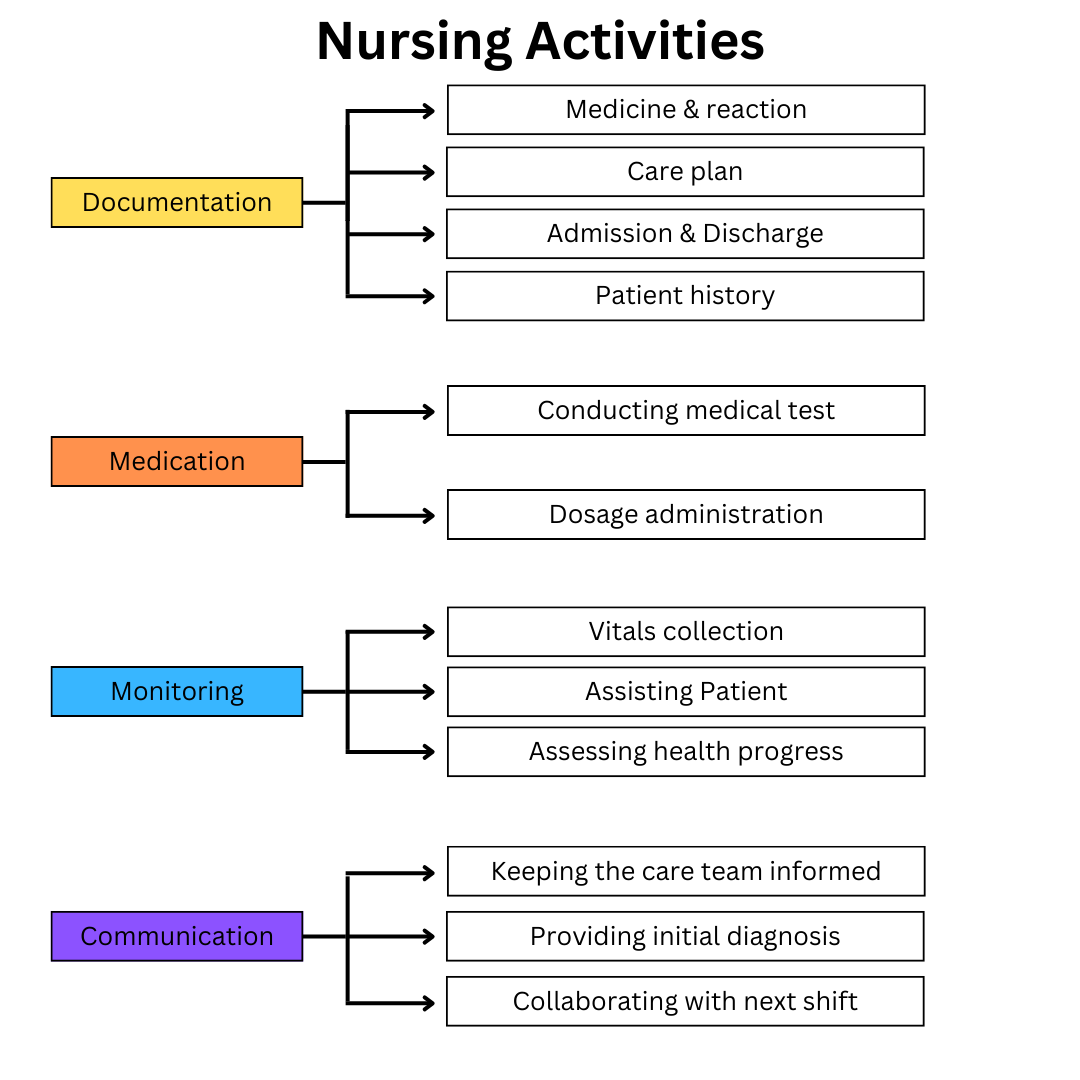
\includegraphics[width=1\linewidth]{images/Nursing Activities.png}
    \caption{Major Nursing Activities that may be Automated to an Extent}
    \label{fig:nursingacts}
\end{figure}
It shows how the nursing care workflow can be divided into 4 main categories. These are not the only activities as nurses are involved in logistics among other activities as well. The activities shown in the figure have been selected because they consume a major portion of a nurse's time.
\subsection{Digitization}
The first step towards any automation is converting the manual workflow and paperwork into digital format. Each step counts towards automation, setting up a path for future efforts to be streamlined. \cite{Study3} conducted an experimental study in 2003. They highlighted the limitations of traditional paper-based nursing records. They further emphasized the need for computerization of nursing records and proposed the use of a terminology-based ENR system. The study consisted of three phases: analysis of nursing notes, development of a terminology server and an ENR, and an evaluation of the system. Nursing notes were decomposed into phrases and cross-mapped with the International Classification for Nursing Practice (ICNP). The terminology server was developed to manage nursing concepts and phrases, whereas the user application system facilitated nursing note documentation. The system was evaluated in two Korean hospitals by 20 nurses documenting nursing notes for 57 patients.\\
Analysis of nursing notes revealed patterns reflecting the nursing care workflow, supporting the feasibility of structuring narrative nursing notes. A total of 14,727 phrases were used to document nursing notes. Among the 259 unique nursing concepts extracted, there were 237 unique phrases identified. The mean time required for documentation decreased significantly from 276s to 158s as users gained experience with the system. The results indicated that the ENR is indeed effective in a clinical setting. Nurses achieved a higher success rate and exhibited rapid adaptation over time. The findings underscore the potential of digital solutions like ENR systems to optimize nursing documentation, freeing up more time for direct patient care and improving patient outcomes. This study aligns closely with our research objectives of exploring automation technologies to enhance nursing care workflow and highlights the importance of digital transformation in healthcare.

% ---------------------------Usability Study-------------------------------------
In 2011 \cite{enr-usability} aimed to evaluate ENR systems and provide guidelines for further development of technologies in nursing. The study incorporated five key attributes specific to ENR systems for its usability evaluation: fluency of reporting practices, accuracy of documentation, adaptability, exploitation of documented information, and support for collaborative care.
The evaluation study was conducted in Finland in 2010, and involved four ENR systems used in various healthcare settings. Contextual interviews were conducted with 18 nurses from different organizations, focusing on documentation practices, practical exercises, and information exchange.
The study revealed that nurses preferred electronic documentation for its accessibility and potential for information reuse, but all evaluated systems exhibited usability problems. Documentation was time-consuming because of poor user interface design and complex interaction sequences. The systems did not align with the nurses' mental models, lacked support for structured templates and copy functionality, and required redundant data entry. Nurses reported difficulties in learning. Accessing and reading documented information was problematic, impacting collaborative care among healthcare professionals. 
The study emphasized the importance of aligning ENR systems with nursing practices and called for a conceptual redesign of these systems. These findings serve as a foundation for evaluating the current state of usability and informing future enhancements in ENR systems. This will become the foundation for the evaluation of our system.

% ---------------------------------Something--------------------------------------
\cite{emr-impact} investigated the impact of Electronic Medical Record (EMR) technology on nursing efficiency through a comprehensive literature review. Utilizing PubMed, Ovid, and general-purpose search engines, the researchers identified 23 relevant articles. By analyzing baseline measurements of nursing efficiency in using the Value Model Realization (VMR) Program, implemented by Texas Health Resources (THR), in hospitals before EMR conversion, the study provided valuable insights into the efficacy of EMR systems in optimizing nursing workflows. The study found that the nurses saved on average 73 minutes in normal wards and 50 minutes in ICUs during their 12-hour shift enabling them to support other initiatives. The study stressed the need for comprehensive understanding and coordination among disciplines for the efficient development of systems to support nursing. 

The studies show that an ENR is a practical solution for automation and it must be pursued but our approach incorporates a vision for activity recognition. To draw a fair comparison we must incorporate systems that automate nursing via sensors and vision. Activity recognition is a complex task. Several studies on major activity datasets for action recognition have been published. On the Kinetics-700 Dataset, a study \cite{InternVideo} achieved the highest accuracy of 84\%. They achieved 91.1\% top-1 accuracy on the kinetics-400 dataset and 77.2\% top-1 accuracy on the something-something v2 benchmark. \cite{ViT} integrated the vision transformer (ViT) and its variant UniformerV2, alongside additional local spatiotemporal modeling modules, to facilitate multi-level representation interaction. By taking advantage of both generative and discriminative self-supervised video learning they achieved 91.3\% accuracy on the kinetics-600 dataset whereas \cite{TubeViT-H} achieved the SOTA accuracy of 91.8\% on the same dataset. While conventional methods only initialize the linear classifier head for vision classification, \cite{ViT} leveraged the text encoder from pre-trained language models for visual recognition tasks. Replacing the classifier with knowledge from the pre-trained language model achieved SOTA. For ActivityNet, which is another popular human activity dataset, they achieved the highest accuracy of 96.9\%. This shows that there isn't a single approach to solving the problem of activity recognition and models have different accuracy when the dataset varies. All these approaches solve the problem of trimmed data. Trimmed data contains clips that are guaranteed to contain an activity within its short duration spanning a few seconds. The SOTA on untrimmed data for temporal activity recognition using the AR@50 metric is 64.28\% on the Thumos14 dataset. The activity in our use case needs to be detected, localized, and recognized for patients in hospital wards therefore an AR@5 metric is a more cohesive choice. With such a metric the accuracy of the existing models drops significantly to a staggeringly low 33\%. Several studies have attempted to recognize activities of daily living.
\subsection{Sensor-based patient monitoring}
\cite{robot-impact} explored the utilization of robots and automated devices in nursing care. The focus was on their impact on nurses' work efficiency and patient outcomes. Most of the 25 studies reviewed were conducted in hospital settings, with some in elderly care centers or nursing homes. The technologies used were categorized into algorithm-based methods, sensor technology, and automatic robotic devices. The most extensive application was in medication care, where robots were employed for automated dispensing systems and bar code-assisted medication administration. These interventions significantly reduced medication errors, improved nurses' working time, and enhanced overall satisfaction. Additionally, robots were utilized for patient monitoring and nursing treatments, showing promising results in reducing nurses' workload and improving patient safety. Use of robots and IoT medical devices can become an extension of our work to better optimize nursing care workflow.

%------------------------SVDD Implementation------------------------
\cite{Study7} proposed a situation-aware abnormality detection system based on Support Vector Data Description (SVDD) for elderly people. The authors emphasized the significance of abnormal activity detection in elderly care as it can help predict diseases and provide timely support. This study aimed to detect abnormal activities in specific situations by analyzing features and designing a zone-based situation detection system. SVDD is employed to detect abnormal activity based on the designed features. The feasibility and accuracy of the proposed method are experimentally evaluated.
The hardware used in the system includes a U-tile sensor network for precise location tracking and a smart plug to monitor home appliance status. The U-tile sensor network utilizes pressure sensors and RFID antennas embedded under the floor to track the position of elderly individuals. The home setup is divided into various zones. The situation is determined based on the zone, status of related devices, actions of the elderly personnel, and environmental factors. The results of the experiments indicate that the system achieves a high accuracy in detecting situations and abnormal activities, with only a few errors detected. The system successfully detected all abnormal activities and provided warning services to remote family members. Future plan is to implement the system in a hospital ward and evaluate its performance in detecting other situations and abnormal activities.

\cite{DDPM} proposed a system to monitor a patient’s condition by monitoring the body temperature and pulse rate. It consists of pulse rate monitoring software and a wearable device that can measure a subject’s temperature and pulse rate using a fingertip only. The wearable device can record the measurement data and interface to a desktop via an Arduino microcontroller. It provides a cost-effective solution due to limited hardware requirements for patient vitals monitoring but is limited to temperature and pulse rate only. In another experimental study, \cite{necklace-sensor} proposed a sensor-based wearable device that allows continuous patient monitoring, specifically in a nursing home setting. The device automatically provides alarms to caregivers based on biosignals measured by sensors integrated into a necklace worn by each patient. The device detects the heart rate, involuntary falls, and the location of the patient within a building. It also has a manual call button. \cite{arduino-remote-monitoring} proposed a framework that integrates web services with multiple sensors controlled by Arduino Uno. Four types of sensors were used to monitor the patient's vital signs such as electrocardiogram (ECG), body temperature, pulse rate, and oxygen in blood (SPO2). The system improves real-time data collection, eliminates manual data gathering, and enables the monitoring of a large number of patients at the cost of integrating sensors with a singular interface chip called an eHealth shield, which then connects with Arduino Uno to send the data to a web service. \cite{jamjoum} proposed a portable patient monitoring system. Blood oxygen saturation levels, electrocardiogram, heart rate, and body temperature were the main vital signs measured. Each vital sign was captured using a sensor connected to a microcontroller with a built-in wireless communication module. The micro-controller processes the vital signs' data and uploads it to the cloud. The user interface was built on three platforms: an Android application, a website, and a hand-held module based on Raspberry Pi. The system captures vital signs and uploads the readings in real-time, enabling medics to monitor and assess a patient's medical condition remotely. Real measurements were taken using the system and compared to readings obtained using appropriate devices in a medical clinic. The results showed that the system could capture the vital signs with a deviation of less than 10\% from the referenced readings. This architecture makes it very suitable for long-distance online patient monitoring. This approach removed the need for an eHealth shield interface that was used in the previous study by Theses studies provide an important insight into how our prototype can be extended to incorporate sensors measuring vital signs.

\cite{smartphone} presented a self-learning scheme for smartphone-based activity recognition aimed at enhancing medical monitoring for patients, particularly postoperative individuals, using data collected from common motion sensors in smartphones. The purpose of the study is to develop an adaptive system capable of recognizing both known and unknown activities without prior knowledge of the latter. The methodology involves preprocessing sensor data to eliminate orientation influence, extracting robust features, and employing a self-learning framework for activity recognition. The self-learning scheme dynamically clusters unknown activity data and assigns new category labels, which are then merged into the training dataset to improve recognition accuracy. Experimental results, conducted with data from postoperative patients performing six labeled daily activities, demonstrate that the proposed scheme achieves high accuracy, surpassing 80\% even when faced with multiple types of unseen activities. The study contributes to the field by introducing a comprehensive self-learning framework for activity recognition using smartphone sensors, aligning with the broader goal of advancing mobile health applications for patient monitoring.

\subsection{Vision-based automation patient monitoring}
A range of studies have explored real-time patient activity recognition using cameras. \cite{Study6} proposed a context-aware human activity recognition (HAR) system using a depth camera to improve the privacy and security of patients. With the use of depth cameras, the image becomes noisy; thus the authors introduce a novel feature selection technique to extract and select the most relevant features for activity recognition. The proposed system is evaluated using hidden Markov models (HMM) and compared to existing works that use depth cameras.\\
The proposed approach starts with an empty model, adding and removing variables based on important tests such as the partial F-test. The alpha-to-enter and alpha-to-eliminate values control the inclusion and exclusion of variables. The step-wise regression built a model that initially includes all independent variables and then eliminates those that are not statistically significant. The proposed approach for feature extraction and selection aims to reduce the feature space to a constrained number of features. It uses FLD and forward-backward regression algorithms.
The authors train and test the proposed approach offline. Future research should implement the proposed approach in an actual clinical setting. The accuracy achieved was not near SOTA techniques that do not cater to privacy. Nevertheless, it has set a benchmark for privacy in activity recognition. This study has shown an important aspect of security and privacy that needs to be considered while monitoring patients. This introduces another challenge for future work, considering that feature extraction through visual input can be cumbersome and significantly reduce accuracy.

\cite{UET-Study} discussed the problem of recognizing abnormal human activities in videos of patients. The authors proposed a multi-class abnormal action detection system that utilizes the You Only Look Once (YOLO) network as a backbone convolutional neural network (CNN) model. The CNN model was trained using a large dataset of patient videos constructed by them. Each frame was labeled. There were 23,040 labeled images of patients’ actions for 32 epochs.
The proposed approach involves dividing the videos into segments and then applying the trained CNN model for classification prediction on each segment. The confidence and prediction scores are calculated based on Intersection over Union (IOU) for all classes. Evaluation metrics, such as accuracy, precision, recall, and F1-score, are then computed into a confusion matrix to assess the performance of the system. The proposed approach achieves a high accuracy of 96.8\% for abnormal action recognition, with an improved F1-score of 89.2\% compared with SOTA techniques. The authors also highlight the limitations of the YOLO model, particularly its inability to predict the number of objects and handle small objects. The paper suggests future work to extend the system's capabilities for handling multiple objects and individuals in real-world scenarios. 
\cite{fuzzy} proposed a fuzzy logic classifier for elderly patient fall detection. The proposed approach involves creating a home surveillance system using ordinary webcams. These webcams track subject movement, and the video stream is processed in MATLAB. After background subtraction and cleaning, relevant parameters (such as center of mass, aspect ratio, body speed, and face speed) are extracted from the image sequences. The system includes feature extraction and classification of events. The authors use a fuzzy logic classifier to tabulate these events according to two decisions: FALL or NON-FALL. The experimental results proved that they could discriminate a falling event from a non-fall situation by combining the different parameters. The authors achieved results with a sensitivity of 92.7\% and a specificity of 99.1\% for fall detection. This helps us extend our future plans to abnormal activity detection using their specific fuzzy logic classifier. 

\cite{neural-network} developed a video-based framework for real-time activity recognition. Simple motion features are modeled over time and classified into different activity levels using a neural network. For the experiments, the Sheffield Activities of Daily Living dataset is used where each activity is simulated within a simulated assisted living environment under two different illumination conditions. Their experiments show that the detection rate for each of the activity levels is well above 80\% and the detection time is approximately 30 seconds. The fact that the dataset contains simulated activities, may not work so well in a real clinical setting and so there is a need to test this approach in a real-world scenario.

\cite{wearable-cams1} presented a novel approach for activity recognition using video data captured by a wearable camera, to assist individuals living with disabilities or the elderly in their daily activities. The purpose of the study is to develop a system capable of remotely identifying specific activities such as drinking, walking, going upstairs, and going downstairs. The methodology involves extracting features using optical flow and applying classifiers such as k-Nearest Neighbors (k-NN), LogitBoost, and Support Vector Machine (SVM), followed by smoothing using the Hidden Markov Model (HMM). Results indicate that average pooling significantly enhances performance, with SVM (RBF kernel) achieving the highest accuracy of 76.7\%. Furthermore, incorporating multi-activity videos into the training dataset improves classification accuracy by an average of 6.2\%. Figures and values provided in the paper illustrate the performance of different classifiers and the impact of feature extraction methods and training data on accuracy. This research provides insights into the development of a wearable camera-based system for activity recognition, which aligns with the broader goal of leveraging technology to assist individuals with disabilities or cognitive impairments in their daily lives.

\cite{wearable-cams2} proposed a novel method for activity recognition in Ambient Assisted Living applications, focusing on analyzing recordings of daily living captured by wearable cameras. The approach involves constructing discriminant object-centric motion descriptors to represent micro-actions within the viewpoint of the action maker, aiding in defining the performed activity. The study utilizes deep learning techniques for object detection and motion analysis, incorporating both Histograms of Optical Flow (HOF) and Motion Boundary Histogram (MBH) descriptors. The results on the ADL dataset show that the proposed method with the MBH descriptor outperforms state-of-the-art approaches in activity recognition.. The paper contributes to the field of activity recognition from egocentric videos, offering insights into behavior monitoring and health applications, which aligns with our future focus on leveraging wearable technology for assisted living environments. 

\section{Current State-of-the-Art}
Aside from systems being researched, some software solutions are being used in the healthcare industry. Some of the popular solutions are listed below.
\subsection{MyChart by Epic}
MyChart lets you see your medications, test results, upcoming appointments, medical bills, and price estimates. It can be integrated with other EHRs such as Cerner Aware to transfer data. It is more patient-oriented and focuses on providing reminders and medication to the patient while providing analytics of medical history only instead of real-time vitals.
\subsection{Cerner}
Cerner Melior is a comprehensive medical record system developed in collaboration with Swedish healthcare. The system provides support for patient care and is used in 32 hospitals across Sweden. It provides real-time vital monitoring by integrating medical devices with a comprehensive dashboard.
Cerner Millennium is aimed at helping in documentation and assessing critical patient data, streamlining workflows, and helping to improve both patient safety and the overall patient experience. It is a little more advanced than its Melior counterpart as it provides an additional feature of patient vitals analytics.
At the heart of Cerner, the Cerner Aware is the main product with the most features that Cerner offers. An environment for multiple EHR integrations. It uses medical Device integration to capture real-time vitals and provide data analytics.
\subsection{MEDITECH Expanse}
MEDITECH Expanse is a web-based EHR. Expanse goes beyond basic record-keeping by offering features that improve clinical workflows and patient care.  Clinicians can leverage mobile capabilities to access patient charts and documentation at the bedside, while features like decision support tools and integrated genomics can aid in informed treatment decisions.  Expanse focuses on patient engagement with patient portal access and aims to reduce the administrative burden for healthcare staff through its user-friendly interface.
\subsection{AthenaOne}
AthenaHealth offers a cloud-based solution AthenaOne, designed to improve efficiency and patient care.  Nurses benefit from features like customizable templates and macros to reduce documentation time, athenaCommunicator for secure patient engagement, and real-time access to patient data through its' app.  AthenaHealth focuses on user experience with features like intuitive workflows and easy navigation, aiming to minimize time spent on administrative tasks and maximize time spent with patients.
\subsection{eClinical Works}
eClinicalWorks is a cloud-based EHR designed to streamline workflows for healthcare providers. This translates to features such as AI-powered documentation tools that simplify note-taking, improved access to patient data anywhere and anytime, and communication functions to collaborate with doctors and patients. eClinicalWorks goes beyond basic EHR by incorporating advanced AI features like "Sunoh" which converts conversations to documentation and an "AI Assistant" for streamlining tasks.
\subsection{PointClickCare}
PointClickCare serves as a comprehensive EHR solution, granting healthcare providers easy access to residents' and patients' medical records, facilitating streamlined medication management, personalized care plans, and efficient billing and financial management. The system also aids in staff scheduling and training, offers health analytics insights, and fosters seamless communication among care teams. With its user-friendly interface and integration capabilities, PointClickCare ensures regulatory compliance, supports remote access, and can be tailored to different healthcare settings, ultimately enhancing the overall quality of care provided.

\subsection{Vocera}
Vocera's solutions for smart nursing involve the use of wearable devices and mobile apps. It allows nurses to communicate with each other and with patients in a voice-activated manner. The Collaboration Suite delivers real-time situational awareness. Vocera Edge is a cloud-based communication solution for smartphones that allows nurses to quickly recognize and respond to changes in a patient's status. It enables them to document EHR, receive filtered alarm notifications, view vital signs, and send secure messages tagged with patient data and care team information.
\subsection{Closer - Elderly Smart Home}
A smart home nursing solution that uses depth sensors to detect abnormal activity. It informs the caretakers and remotely located nurses. Comes embedded with an EHR system that provides real-time health conditions to caretakers. It doesn't use any RGB cameras and is integrated with medical devices to extract vitals. 
\subsection{Smart Peep}
It utilizes computer vision to detect abnormal behavior in real-time such as falls, motionless anomalies, and unusual absences. It then alerts the caretakers to take action. It is more home-oriented and does not involve any vitals monitoring. 
\section{Comparison}
Table \ref{tab: comparison} presents a comparison of the relevant products in the market. Each system is either an EHR, a Medicine Management System, or a Telehealth system. They either utilize their own custom-made hardware vital collection devices or integrate them with existing medical devices. 
The top 3 have been selected specifically which take up roughly 70\% of the market. Studies have shown that nurses tend to prefer paper-based documentation over electronic systems simply because they fail to provide the best and easiest user interface and experience. Some of the following products provide a cluttered but comprehensive dashboard with low personalization.  The products also fail to provide nurses with task organization and prioritization. They also integrate medical devices which is an accurate form of data collection but is costly.

\begin{table}[h]
\centering
\caption{Comparison of Features Offered by Popular Healthcare Solutions}
 \resizebox{\columnwidth}{!}{%
 \renewcommand{\arraystretch}{1.5} 
            \begin{tabular}{|m{3cm}|>{\centering\arraybackslash} m{2.5cm}|>{\centering\arraybackslash} m{2.5cm}|>{\centering\arraybackslash} m{2cm}|>{\centering\arraybackslash} m{2cm}|>{\centering\arraybackslash} m{2cm}|>{\centering\arraybackslash} m{2.5cm}|}
            \hline
            \textbf{\large Products} & \textbf{Activity recognition} & \textbf{Realtime monitoring} & \textbf{Task alerts} & \textbf{Detailed dashboard} & \textbf{Patient Analytics}& \textbf{Forecasting} \\
\hline
 \large Epic  & x & \checkmark & \checkmark & \checkmark & \checkmark & x \\
\hline
\large Cerner  & x & \checkmark & \checkmark & \checkmark & \checkmark & x \\
\hline
\large Meditech  & x & \checkmark & x & \checkmark & \checkmark & x \\
\hline
\large Athena health  & x & \checkmark & x & \checkmark & x &x\\
\hline
\large eClinical works & x & \checkmark & x & \checkmark & x & x\\
\hline
\large Point click care  & x & \checkmark & \checkmark & \checkmark & x & x\\
\hline
\large Vocera  & x & \checkmark & \checkmark & x  &  \checkmark & x\\
\hline
\large Closer  & \checkmark & \checkmark & x & x & \checkmark & x \\
\hline
\large Smart Peep  & \checkmark & \checkmark & x & \checkmark & \checkmark & x \\
\hline
\large Nursing portal & \checkmark & \checkmark & \checkmark & \checkmark & \checkmark & \checkmark \\
\hline
\end{tabular}
}
\label{tab: comparison}
\end{table}
\section{Discussion}
In examining the literature about the transformation of nursing care workflow, several key technological advancements emerge. Digitization, exemplified by studies such as Cho et al. (2003) and Viitanen et al. (2011), showcases the shift from manual paper-based records to electronic nursing records (ENR) systems. These systems not only optimize nursing documentation but also significantly reduce documentation time, as evidenced by Cho et al.'s findings. However, challenges in usability and alignment with nursing practices, highlighted by Viitanen et al., underscore the need for user-centered design in ENR implementation. Additionally, the integration of electronic medical record (EMR) systems, as explored by Thompson et al., demonstrates substantial time savings for nurses and emphasizes the importance of interdisciplinary coordination in technology adoption. Concurrently, sensor-based patient monitoring technologies, as investigated by Kangasniemi et al. and others, offer promising avenues for improving medication administration, patient monitoring, and fall detection, thus reducing nurses' workload and enhancing patient safety. Regarding temporal action recognition methods, studies by Siddiqi et al., Gul et al., and Zhan et al. reveal innovative approaches using depth cameras and wearable cameras for real-time patient activity recognition, addressing privacy concerns and improving monitoring accuracy. Looking forward, integrating these technologies into nursing workflows holds significant potential for optimizing patient care and informing future research endeavors in healthcare innovation.

Studies show conflicting results at times when ENRs are used. It cannot be conclusively said that the results from the study conducted by \cite{Study3} will be sustainable on a larger scale. The scope of the study was limited to two Korean hospitals and 20 nurses. They may have a higher success rate and improved patient outcomes, but the results can be detrimental if the software is not designed keeping the nurses' mental model in mind. Usability has been a major concern of the nurses so any future system that is developed should be strictly cohesive with the nursing care workflow while allowing for personalization of its interface as well. The application should be easy to navigate. 

Although a novel approach, there were issues with the proposed methodology of \cite{Study7}. While SVDD is a powerful tool for anomaly detection, its performance could be influenced by the choice of features and the quality of the dataset used for training. Without a thorough discussion of feature selection and dataset characteristics, the robustness and generalizability of the proposed method remain unclear. Additionally, the study relies on hardware components such as U-tile sensor networks and smart plugs for data collection, which may introduce practical challenges related to installation, maintenance, and scalability, particularly when deploying the system in real-world healthcare environments. 

While Azizulkarim et al's system offers simplicity and affordability, it is limited to monitoring only two vital signs. Hameed et al's proposed integration with a singular interface chip may pose scalability challenges. In contrast, Jamjoum et al. presented a portable patient monitoring system capturing vital signs like blood oxygen saturation levels, ECG, heart rate, and body temperature, with data uploaded in real-time to facilitate remote monitoring by healthcare providers. This system, leveraging wireless communication and cloud-based storage, offers a scalable solution suitable for long-distance patient monitoring.
The monitoring and logging of a patient's activity and vital signs is the second most important task. It was noted that using depth sensors instead of cameras for activity recognition may result in lower accuracy of temporal activity recognition, particularly when considering privacy concerns. Systems that have higher accuracy use a multitude of sensors such as floor pressure tiles and IoT home appliances to gather as much information about the patient and location to access the patient status. This leads to an expensive solution and requires specialized hardware which may not be as readily available as cameras are. Some systems that utilize only cameras and achieve high accuracy are slow in their response failing to achieve true real-time monitoring. 

In a clinical setting, a system with minimal lag must be put in place that leverages the existing and prevalent infrastructure to provide a cost-effective and feasible solution that provides patient activity recognition, forecasting, assistance with nursing care workflow, and a comprehensive patient analytical dashboard similar to that found in EHR solutions today. A major amount of research needs to be conducted in temporal activity recognition and forecasting patient activities. 


% Write in your chapter title to set the page header % Literature Review

% Chapter 1

\chapter{Datasets} % Write in your own chapter title
\label{Chapter3}
\lhead{Chapter 3. \emph{Datasets}} 
\section{Kinetics-600}
The \textbf{Kinetics-600} \cite{kinetics-600} is an action recognition dataset that consists of approximately 500K videos from 600 action categories each containing at least 600 videos. Each video in the dataset is a 10-second clip of an action moment from a YouTube video. This was an extension of the Kinetics-400 \cite{kinetics-400} dataset. The goal of the Kinetics project was to replicate 1000 classes, each with 1000 image examples like in ImageNet.

There were two main bottlenecks in the Kinetics-400 dataset: 

(i) Identifying relevant candidate YouTube videos for each action class

(ii) Find classes with many candidates. 

The last 10 seconds of YouTube videos were taken as clips. They had a variable resolution and frame rate. For the action class, all clips were taken from different YouTube videos. In this dataset, the number of classes has increased by 50\%, from 400 to 600, and the number of video clips has increased by 60\%, from approximately 300k to approximately 500k.

Although the dataset has 600 classes of activities, it does not have the exact activities that we require for our application. It contains a few activities somewhat similar to the ones we would like to detect such as we want to detect talking which exists as “talking on a cell phone.” For eating it has classified the activity based on different foods, such as spaghetti, carrots, burger, chips, ice cream, hotdog, watermelon, doughnuts, and cake. For a person walking, the dataset refers to the activity of walking a dog or walking with a horse. For fall detection, it addresses only falling from a chair or falling from a bike but the latter is not of use to us. The only activity that may match our use case is the sleeping activity which is included in the dataset. 

 The dataset was split into 392,622 clips that were used for training, 30000 for validation, and 60000 for testing. The clips unlike in Kinetics-400 do not contain multiple activities such as “texting” while “Walking” as the data collection methodology changed removing such anomalies. The data collection process is as follows:

 As in Kinetics-400 a class list for human actions was decided using multiple sources such as past action datasets, motion capture datasets, and crowd-sourcing systems such as Amazon Mechanical Turk (AMT). The key difference with the Kinetics-600 datasets is that many classes were sourced from Google’s Knowledge Graph and YouTube’s search box auto-complete; for example, an object or a verb was typed and auto-complete suggestions were followed up to see if they contained enough videos of the same action to decide whether or not that class would be a part of the dataset. For the Kinetics-400 dataset video titles were matched with action lists. Image classifiers extracted the clips where an activity was detected. Every clip used originated from a different YouTube video. AMTs then labeled the clips and identified whether a specific action was occurring in the clip's duration. Only the clips with 3/5 positive responses were added to the dataset. For the Kinetics-600 dataset, a set of queries was prepared for each class in the two most spoken languages, English and Portuguese. As an example, the queries for the folding paper were: “folding paper” (en), “origami” (en), and “dobra papel” (pt). Instead of matching the textual queries directly weighted n-gram representations of the combination of the metadata of each video and the titles of related videos were used. Combined, with standard title matching, a robust similarity score between a query and all YouTube videos was obtained.
The dataset was then cleaned up in the last stage. Duplicates were removed from the dataset by comparing the similarity score between feature vectors. Noisy classes were either merged or removed. Final filtering was performed by sorting examples in decreasing order of confidence. The dataset file contained a field named “label”, YouTube ID, time start and time end (in seconds), and "split" that identified whether the sample was for testing, training, or validating data.
\section{Kinetics 700}
After Kinetics-600, the Kinetics-700 \cite{kinetics-700} dataset was released comprising 700 action classes, each with at least 700 video clips. From the dataset, 545793 clips are used for training, 35000 for validation, and 70000 for testing.  Synonyms and searches in different languages i.e. English, French, Spanish, and Portuguese are used to get more clips for the rarest classes. Duplicate clips are removed by clustering the clips. The dataset contains a label that indicates the activity performed, YouTube ID time and start and time end (in seconds), and split to tell if it is testing, training, or validating data.  
\section{Toyota Smart Home Dataset}
The Toyota Smarthome dataset was captured in a residence with seven Kinect v1 cameras. It comprises 31 activities of daily living of 18 senior citizens between the ages of 60 and 80. The activities are recorded in 3 different scenes from 7 camera viewpoints. Each person is recorded for 8 hours in one day from morning until the afternoon. The dataset has a 640x480 resolution and three modalities: RGB, Depth, and 3D Skeleton. RGB was used to extract the 3D skeletal joints. The persons' faces are blurred for privacy concerns. The dataset is available in two versions: Trimmed Toyota Smarthome \cite{Das_2019_ICCV} and Untrimmed Toyota Smarthome (TSU) \cite{dai2022toyota}. We use the untrimmed dataset version, and particularly the Balanced Untrimmed dataset to train our forecasting model.
\begin{figure}[h]
    \centering
    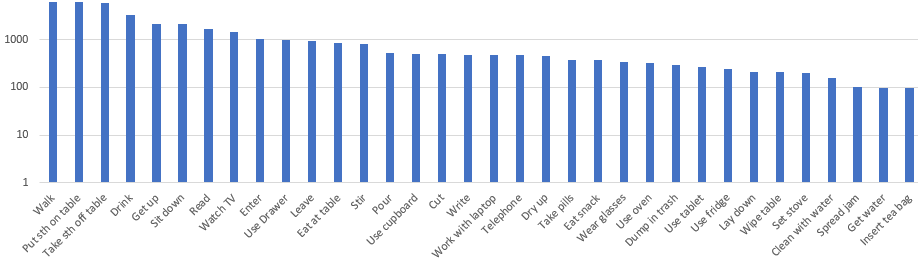
\includegraphics[width=0.8\textwidth]{images/Balanced_TSU.PNG}
    \caption{Activities Involved in Balanced Untrimmed Dataset}
    \label{fig:balancedtsu}
\end{figure}
The original Toyota untrimmed smart home video dataset has close to 51 actions and the frequency of the occurrence of these actions in the videos is highly unbalanced which means that certain actions occur more frequently than others. Therefore, certain low-frequency actions were removed and a final balanced dataset consisting of only 34 highly occurring actions was created. Balanced TSU shares the same untrimmed videos as fine-grained TSU: 536 videos with 21 21-minute average duration. Activities were carried out in a highly spontaneous way. The activities involved in the Balanced Untrimmed dataset are shown in figure \ref{fig:balancedtsu}. The activities that are within the project's scope are: \\
Walk, drink, get up, sit down, take pills, eat, eat a snack, read, watch TV, leave, lay down.

\section{THUMOS14}
The \cite{thumos-14} dataset serves as a cornerstone for training the Boundary Sensitive Network (BSN) for temporal action proposal generation. THUMOS14 is a comprehensive dataset specifically designed for temporal action localization tasks. It contains over 254 hours of video data across 101 action classes. It has annotated splits, including training, validation, background, and test sets. THUMOS14 provides a robust platform for evaluating the effectiveness of action recognition algorithms. The dataset offers spatio-temporal annotations and pre-extracted features, enhancing its utility for training and testing various models. THUMOS14 remains a widely adopted standard in the field due to its extensive content and well-defined evaluation protocols, making it an ideal choice for training the BSN model in this study.

The dataset boasts meticulous curation and annotation, ensuring its suitability for training and evaluating action localization algorithms. With over 254 hours of video data, comprising approximately 25 million frames, THUMOS14 offers a substantial corpus for temporal action localization tasks. This dataset is carefully categorized into distinct splits, including a comprehensive training set with over 13,000 temporally trimmed videos covering 101 action classes, a validation set featuring over 1,000 untrimmed videos with temporal annotations, and a background set containing over 2,500 videos devoid of any of the 101 action classes to prevent false positives. The test set comprises 1,500 untrimmed videos with withheld ground truth labels, allowing researchers to benchmark their models' performance on unseen data. The data collection process for THUMOS14 involved sourcing videos from YouTube reflecting real-world scenarios and ensuring the dataset's relevance and applicability to practical action recognition tasks. THUMOS14's well-defined evaluation protocols encompass a range of metrics tailored to assess temporal action proposal generation algorithms' performance accurately. The protocols include metrics such as mean Average Precision (mAP) and Intersection over Union (IoU), providing researchers with clear guidelines for assessing and comparing the efficacy of different models trained on the dataset.

\section{AVA-Kinetics}
The AVA-Kinetics dataset \parencite{ava-kinetics} is a comprehensive video dataset focused on human actions. It merges the AVA dataset and the Kinetics-700 dataset by applying AVA-style annotations to Kinetics-700 videos. The AVA dataset includes 80 different actions across 430 video clips, each lasting 15 minutes. Annotating the AVA dataset is costly because it involves marking actions for each person in a video clip at a one-second interval. It also involves generating a bounding box around each individual to assign multiple concurrent activity labels. The dataset is divided into 141,475 clips for training, 32,592 clips for validation, and 64,902 clips for testing.
Initially, a pre-trained Faster RCNN detects the frame with the individuals and highest detection score. Human annotators then add any missing bounding boxes in the data. A 2-second video segment centered around this keyframe is extracted, and at least three human raters propose action labels for the person in that keyframe. These labels are later verified by two to three additional raters.
The dataset includes 27 AVA classes with low recognition accuracy and 115 related classes from the Kinetics dataset. The dataset file contains several details: a video ID (identifier on YouTube), the timestamp of the middle frame (in seconds from the video's start), the bounding box coordinates of the person (x1, y1, x2, y2), an action ID for the performed action, and an optional person ID linking bounding boxes if depicting the same individual. 

\section{ImageNet}
The ImageNet dataset \parencite{image-net} stands as a monumental cornerstone in computer vision research, constituting a vast image database structured according to the WordNet hierarchy. With an ambitious goal to furnish approximately 1,000 meticulously annotated images for each synset in WordNet, ImageNet boasts tens of millions of meticulously labeled images encapsulating a diverse spectrum of concepts. Its inception stemmed from the imperative to address two critical exigencies in the field: firstly, establishing a quintessential benchmark task for computer vision—the North Star Problem—choosing object categorization as the central challenge, and secondly, mitigating the paucity of data requisite for fostering generalizable machine learning methodologies, especially in light of the burgeoning digital data landscape. While the precise methodologies employed for image collection remain undisclosed to the public, it is inferred that images were procured from myriad online sources, likely through web searches and image scraping, with a rigorous quality control mechanism ensuring image fidelity. Human annotators meticulously categorized images into their corresponding synsets, augmenting an automated process that handled the sheer scale of data. The profound impact of ImageNet on computer vision research, particularly in catalyzing advancements in deep learning, cannot be overstated. Deep convolutional neural networks, pivotal to contemporary breakthroughs, owe a debt to ImageNet's extensive labeled data. Nevertheless, contemporary discourse has surfaced criticisms regarding potential biases and limitations within the dataset, stimulating a quest among researchers for more inclusive and expansive datasets to propel the field forward.

\section{ActivityNet-1.3}
Many existing datasets are quite basic. In contrast, the ActivityNet dataset \parencite{activity-net} is a comprehensive, video-based dataset that encompasses a wide array of intricate activities. It comprises 203 activity classes, each class having an average of 137 untrimmed videos. On average each video contains 1.41 instances of activities, making up a total of 27,801 videos and 849 hours of footage. This dataset is the first extensive human activity database to categorize a substantial number of videos using a semantic taxonomy. Crafting a semantic framework for activities is complex, so this dataset utilizes the Department of Labor's activity taxonomy from the American Time Use Survey. It contains over 2000 activities out of which only 203 activity categories were chosen. Activity classes are organized into seven top-level categories: Personal Care, Eating and Drinking, Household, Caring and Helping, Working, Socializing and Leisure, and Sports and Exercises.

The data collection process follows several stages. Initially, videos are sourced from YouTube by searching for specific activity labels. These videos are then verified by Amazon Mechanical Turk, who ensure that each video contains the intended activity. Non-compliant videos are excluded.  Only experienced workers are employed to ensure integrity. Turkers then manually annotate the segments of the videos where the desired activities occur. A single video can include multiple activity labels. The dataset file contains labels, duration, start and end times (in seconds), the subset type, and a URL linking to the video on YouTube. 50\% of the dataset is used for training, 25\% for validation, and the remaining 25\% for testing.

\section{HACS}
The Human Action Clips and Segments (HACS) dataset \parencite{HACS} is designed for human action recognition in videos. Utilizing 200 action classes similar to those in ActivityNet. The dataset was compiled by querying YouTube with these labels, resulting in an initial collection of 890,000 videos. After removing duplicates, the dataset includes 504,000 clips, each averaging 2.6 minutes in length.
This dataset features two types of manual annotations. The first type involves action labels on 1.5 million 2-second clips extracted from the videos. These clips are included by comparing results from various visual classifiers. The second type, HACS Segments, focuses on temporal localization within 50,000 untrimmed videos, ensuring each video contains at least one action segment. The segments in HACS are shorter in comparison to ActivityNet with 4.7 times more segments and 2.5 times more videos.
The dataset file includes: the class name, YouTube ID, a subset designation (training, validation, or testing), and start and end times (in seconds). A label of 1 denotes a positive sample, while -1 indicates a negative sample.
The authors have divided the dataset into a training set comprising 1.4 million clips sourced from 492,000 videos and a validation and testing set with 50,000 clips each.

\section{MMACT}
The MMACT dataset \parencite{MMAct} is a large-scale collection designed to improve action detection and recognition. It includes over 36,000 action instances across 37 classes, covering tasks like desktop activities and check-in procedures. The dataset features seven types of data modalities. Twenty subjects participated, wearing smart glasses for egocentric videos, carrying smartphones with sensors in their pants, and wearing smartwatches. The data was collected in four indoor settings: free space, occlusion areas, entrances, and desk work. Research shows the dataset is effective for studying actions across different subjects, scenes, views, and sessions. The MMACT dataset provides a diverse and detailed resource for action recognition studies.

\section{IKEA ASM}
IKEA ASM \parencite{IKEA} is a video dataset focused on assembly tasks. It aims to help analyze and understand human activities through actions, objects, and poses. The dataset includes 371 samples of furniture assembly with ground-truth annotations. Each sample features three RGB views, a depth stream, atomic actions, human poses, object segments, object tracking, and camera calibration data. Forty-eight participants assembled furniture in different locations: offices, labs, and homes. The data was collected using three Kinect V2 cameras placed to capture the work area from the front, side, and top. The dataset includes 16,764 annotated activities, with each action averaging 150 frames or 6 seconds.

\section{Home Action Genome}
The Home Action Genome dataset \parencite{home-action-genome} is used for action recognition in multi-view video databases of indoor activities. Data was collected from 27 participants in two houses, capturing diverse viewpoints for both low-level and high-level actions. The dataset includes recordings from 27 types of sensors, such as RGB cameras, infrared sensors, microphones, RGB lights, regular lights, accelerometers, gyroscopes, human presence detectors, magnets, air pressure sensors, humidity sensors, and temperature sensors. These sensors were placed in various locations around the houses and on participants' heads. The dataset provides three types of labels: video-level activity labels, temporally localized atomic activity labels, and spatio-temporal scene-graph labels. It includes annotations for 75 different activities.

\section{UR Fall}
UR-Fall consists of 70 sequences: 30 fall events and 40 daily living activities. Falls are recorded with two Microsoft Kinect cameras and an accelerometer. Daily living activities are captured using one camera (camera 0) and an accelerometer. Sensor data comes from PS Move (60Hz) and x-IMU (256Hz) devices. Each entry in the dataset includes sequences of depth and RGB images from cameras 0 and 1, which are placed on the floor and ceiling, respectively. It also contains synchronization and raw accelerometer data. Video streams are saved as PNG image sequences in separate zip files, with depth data in PNG16 format. 

\section{VidSitu}
VidSitu \parencite{VidSitu}  is a dataset designed for semantic role labeling in videos. It includes a large collection of video data with 29,000 movie clips, each 10 seconds long. Every 2 seconds of the clip is annotated with a verb and semantic roles. Entities are tracked across different events in the same clip. The events are linked through event-event relations. The clips are taken from a set of 3,000 videos and feature a variety of actions, with each video containing an average of 4.2 unique verbs.  200 verbs have more than 100 annotations each, making the dataset both complex and diverse.

\section{WISDM}
\cite{WISDM} "WISDM Smartphone and Smartwatch Activity and Biometrics Dataset" includes data from 51 subjects performing 18 different tasks for 3 minutes each. Data was collected using smartwatches and smartphones in controlled lab settings. Subjects engaged in activities such as walking, jogging, using stairs, sitting, standing, typing, clapping, and eating pasta. These activities fall into three categories: \\
(i) Activities not involving hands. (ii) General hand-focused activities. (iii) Eating-related hand activities\\
The accelerometer and gyroscope on both devices recorded raw time-series sensor data at a rate of 20Hz.  

\section{UCI-HAR}
The UCI-HAR \parencite{UCI-HAR} dataset records data from people wearing smartphones on their waists. These phones have two sensors. Thirty people aged 19-48 participated. Each person performed six activities: Walking, walking upstairs, walking downstairs, sitting, standing, laying.

The smartphone sensors are an accelerometer and a gyroscope. They record linear acceleration and angular velocity at 50Hz. A video captures the activities. Features are generated from the sensor data for the six activities. The dataset uses features from the accelerometer and gyroscope sensors. The acceleration signal is split into body and gravity signals using a Butterworth Filter. Jerk signals are also calculated.

\section{Opportunity}
The Opportunity \parencite{opportunity} dataset is designed to develop activity recognition algorithms using motion sensor data. It contains 2551 instances and 242 attributes. The dataset includes numerous activity instances and sensors of various types, simulating real-world data. It is also used for classification, automation segmenting, sensor selection, and feature selection.
Data was collected from three types of sensors: Body-worn sensors, object sensors, and ambient sensors
\end{enumerate}
Body-worn sensors have 145 attributes, object sensors have 60 attributes, and ambient sensors have 37 attributes. The setup includes 73 sensors with 10 modalities placed on the body, in the environment, and on objects. Subjects perform activities in a room with a deckchair, kitchen, door, coffee machine, chair, and table. Activities of daily living are recorded and synchronized with video footage.
Four people participate, each performing activities naturally and in scripted drills. The dataset includes 25 hours of data and is categorized into five tracks: Locomotion (e.g., sitting, standing), High-Level Activities, Left Arm movements and Right Arm movements.

\section{USC-HAD}
The UCS-HAD \parencite{USC-HAD} dataset is used to compare different algorithms in healthcare scenarios. It aids in creating a robust recognition system by training on a diverse group of people. Fourteen subjects, including 7 males and 7 females aged 21-49, participated. Their heights ranged from 160-185 cm, and their weights from 43-80 kg. The experiment involved the activities: Running, Jumping, Sitting, Standing, Walking,  Sleeping, Elevator Up, Elevator Down.
Each subject wore a mobile phone pouch at their front right hip with an embedded MotionNode. It is a motion-sensing application that sends data to a laptop. Subjects held a miniature device in one hand and performed 5 trials of activities on different days. The experiment was recorded and segmented based on start and end points noted by the observer. Each activity trial was saved in a separate file. The .mat file includes information such as height, weight, date, serial number, activity name, activity number, sensor location, orientation, and readings.

\section{Rose NTU}
The Rapid Rich Object Search lab has two datasets. One dataset includes 60 action classes and 56,880 RGB video samples. The activities fall into three categories: daily actions, mutual actions, and medical conditions. Each dataset is captured simultaneously by three Kinect V2 cameras. The RGB videos have a resolution of 1920x1080 pixels, while depth maps and infrared videos have a resolution of 512x424 pixels. The 3D skeletal data provides the 3D coordinates of 25 body joints in each frame. Examples of actions include: staggering, falling down, headache, chest pain, drinking water, standing up, sitting down, eating a meal, and opening a bottle.

\section{PAMAP2}
The PAMAP2 Physical Activity Monitoring \parencite{pamap} dataset is used for activity recognition and intensity estimation. This involves data processing, segmentation, feature extraction, and classification. The experiment includes 9 subjects wearing 3 inertial measurement units (IMUs) and a heart rate monitor. These subjects perform 18 activities, such as cycling, walking, and playing soccer. Each subject wears one IMU on the wrist, one on the chest, and one on the dominant ankle. The heart rate monitor samples data at 9 Hz. The dataset records the subjects performing these 18 activities. % Dataset

% Chapter 1

\chapter{Methodology} % Write in your own chapter title
\label{Chapter4}
\lhead{Chapter 4. \emph{Methodology}} 
\section{Overview}

IP Cameras were wall mounted in the room of the patient for visual input. The video stream is sent at desktop application via an internet connection. Here the activity recognition algorithms namely, the Boundary Sensitive Network (BSN) and Temporal Segment Network (TSN) work in tandem to recognize the activity of the person. The Activity logs generated from these algorithms were then sent to a Django backend via HiveMQTT and Pusher Websockets. This double setup allows for higher throughput. 
\begin{figure}[H]
    \centering
    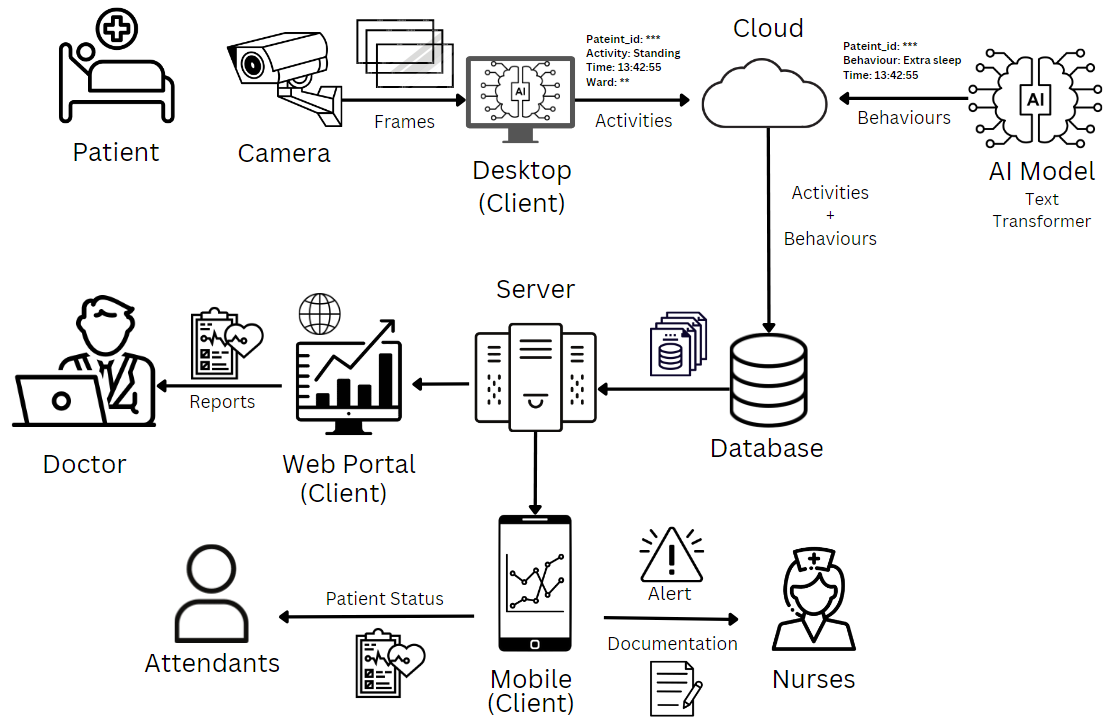
\includegraphics[width=0.8\textwidth]{images/arch.png}
    \caption{Project Process Flow}
    \label{fig:mesh1}
\end{figure}
The activities are stored in the InfluxDb Cloud and  processed by a time series text transformer to forecast patient activities. The admin on the other creates an account and sets up Doctors, Nurses and Patients on the web portal developed in ReactJs. The portal uses HTTPs connections to establish a secure connection with the Django Web app. It authenticates and authorizes each user before allowing access to any requested resources. The dashboard shows the patient's next forecast activity from the current logs. An API call to a web app responds to the user with patient logs in tabular form and Gemini's analytical response to any prompt from the user. When a reading has been missing for more than an hour or  unidentified consumption is perceived, Firebase is used to send push notifications to nurses to prompt  manual logging. The patient's attendants and relatives may also login via patient credentials on the mobile app to check the patient's status remotely. The overall data flow is shown in figure \ref{fig:mesh1}
\begin{figure}[H]
    \centering
    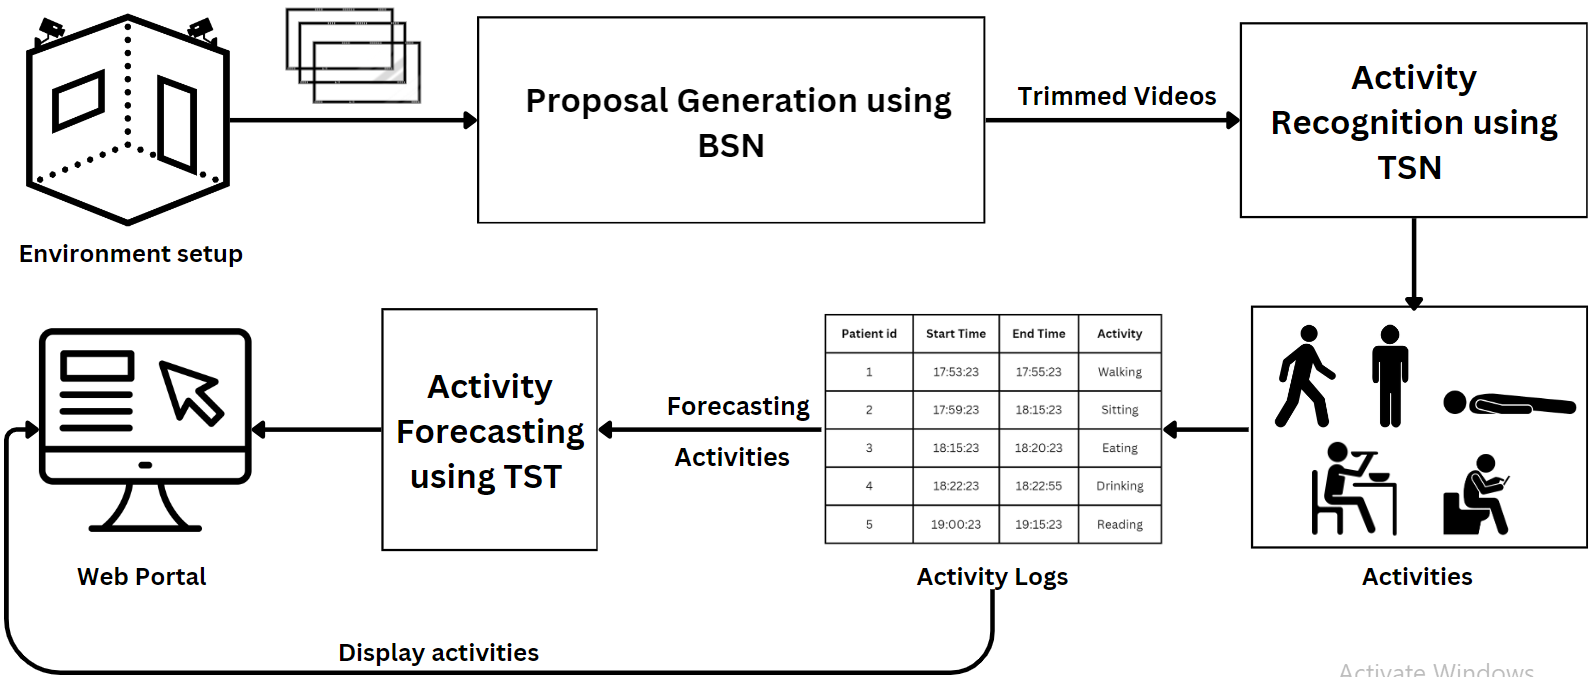
\includegraphics[width=\textwidth]{images/archdia.png}
    \caption{High Level Architecture}
    \label{fig:level 0 diagram}
\end{figure}
At the algorithmic level, figure \ref{fig:level 0 diagram} shows how the video stream is converted to useful information for the doctor. The frames received from the environment are first passed to the BSN for activity localization. The model generates proposals for the incoming video which is then sent to the TSN model. These proposals define the duration in which certain activities have occurred. The TSN model uses these proposals to extract a portion of the video and recognize the activity from the video. Once the current frames are recognized, the subsequent incoming frames are processed. The textual logs generated are then displayed on the web portal and  used to forecast patient activity which is also displayed to the user.

\section{Activity Recognition}
        To understand the purpose of each algorithm better, the types of algorithms must be explained prior to any in-depth dive into a concept. When a person moves a leg it becomes an action which can be labeled as "moving leg". Combining multiple actions such as moving both legs one after another makes an activity which can then be labeled as "walking". Once an activity is performed over a longer duration, it becomes a behavior and generates patterns that can be analyzed. Recognition refers to the identification type of anything. The problem of action recognition and activity recognition has long been solved on trimmed data where videos are small clips of not more than 10 s where an activity starts at the beginning of the clip and ends at the end of the clip. When we pass untrimmed videos or  video streams, we introduce two problems. Activity Detection and Localization. Detection refers to whether an activity is occuring. Localization refers to the identification of the time period during which an activity occurs. After these first two problems are solved, only action recognition, which is a process of classifying and labelling an activity can be processed. 
\begin{figure}[H]
    \centering
    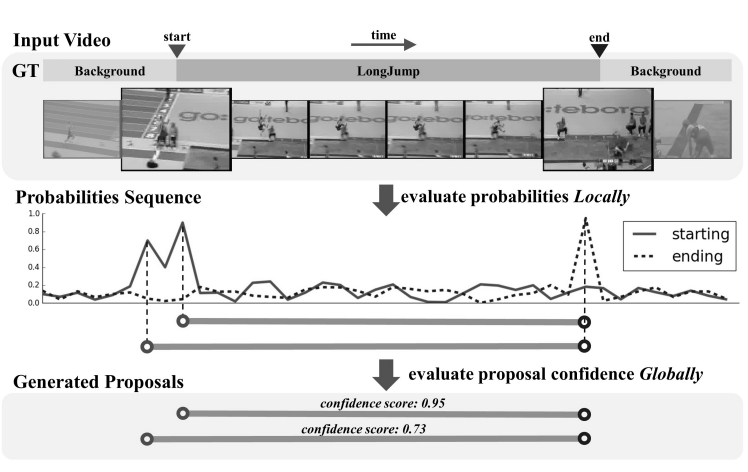
\includegraphics[width=\textwidth]{images/overviewBSN-modified.png}
    \caption{Overview of BSN}
    \label{fig:bsn overview}
\end{figure}
        A boundary sensitive network is used for temporal action proposal generation as shown in figure \ref{fig:bsn overview}. This process is divided into two parts. The first part contains temporal action detection, where the objective is to identify the action areas within the untrimmed videos. This section also provides temporal boundaries and action classes. This step allows for the detection of actions areas throughout the entire video. The second part of the process contains the classification of the action areas identified by the first part of the video stream, each containing a single action. By combining these two components, the methodology provides an approach to action proposal generation. 

\subsection{Properties of proposals}
\begin{itemize}
    
    \item  The proposed system should be capable of capturing actual action instances without generating numerous proposals. 
    \item  The system should also be capable of achieving accurate temporal alignment with ground truth action instances while generating a minimum number of proposals.Thus, the computational cost is reduced because fewer proposals require fewer resources.
\end{itemize}

\subsection{Problem Definition}
The untrimmed video sequence is represented as:
\begin{equation}
X = \{x_n\}^{\text{lv}}_{n=1}
\end{equation}
where, lv is the total number of frames. \(x_n\) is the nth frame in \(X\). Annotation of untrimmed video \(X\) is contained in a set of action instances 
\begin{equation}
    \Psi_g = \{\phi_n = (t_{s,n}, t_{e,n})\}^{N_g}_{n=1}
\end{equation}
where \(N_g\) is the total number of true action instances in a given video sequence \(X\). The starting and ending times of the action instances were \(t_{s,n}\) and \(t_{e,n}\), respectively. The set of annotation \(\Psi_g\) is used during the training process. During the prediction, the set of predicted annotations \(\Psi_p\) should cover \(\Psi_g\) with high precision.
\subsection{Video Features Encoding}

The two-stream network is  divided into two branches:  spatial  and  temporal networks. The spatial network is used to recognize the appearance features of objects and it operates step-by-step on a single RGB frame. In contrast, a temporal network focuses on extracting motion information by working with stacked optical flow fields as shown in figure \ref {fig:encoding-of-vedio-features}. 
\begin{figure}[H]
    \centering
    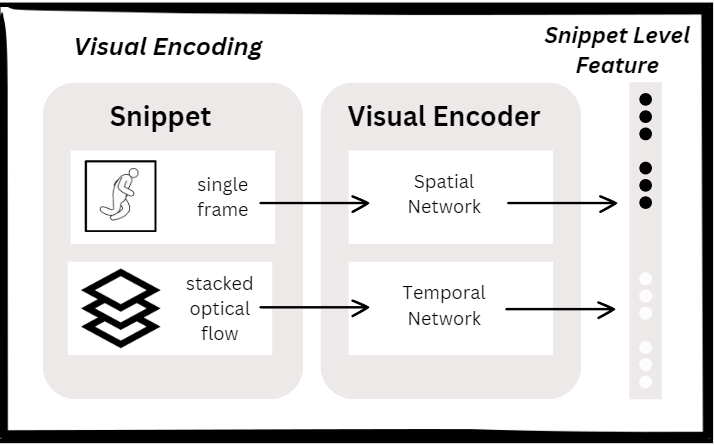
\includegraphics[width=0.7\linewidth]{images/ti1.png}
    \caption{Encoding of Video Features}
    \label{fig:encoding-of-vedio-features}
\end{figure}
This illustrates the movement between different frames. The output scores from both networks are then combined to create an encoded feature vector for each snippet. This vector, concatenates the spatial and temporal network outputs for all the snippets in the dataset. These two-stream feature sequences are very important, because they serve as inputs for the  Bounding Box Selection of the methodology. The integration of spatial and temporal information enhances the overall understanding and analysis of the video data.
Mathematically, the snippet sequence of  vedio is represented as:
\begin{equation}
    S = \{s_n\}^{\text{ls}}_{n=1}
\end{equation}
Here, the length of snippets sequence is represented as ls.
\begin{equation}
    s_n = (x_{t,n}, o_{t,n})
\end{equation}
The snippet above contains two parts. The first part  \(x_{t,n}\) is the spatial network. Here, \(x_{t,n}\) is the \(t_n-th\) RGB frame in Video X. It is used to recognize the appearance features of an object in a video. By contrast,  \(o_{t,n}\) focuses on extracting motion information by working with stacked optical flow fields. Snippets after a regular frame interval are:
\begin{equation}
    ls = \frac{lv}{\sigma}
\end{equation}
We concatenated the output of the spatial and temporal networks to form the encoded feature vector. This vector is represented as:
\begin{equation}
    ftn = (fS_{t,n}, fT_{t,n})
\end{equation}
Here,\(fS_{t,n}\) and  \(fT_{t,n}\) are the outputs of the spatial and temporal processes respectively, for all the snippets, the feature vector is represented as:
\begin{equation*}
    F = \{ftn\}^{ls}_{n=1}
\end{equation*}
This feature vector is used as an input to BSN.

\subsection{Temporal evaluation module}
The temporal evaluation module was used to evaluate the probabilities of the starting, ending, and actionness of events at all  temporal locations. This module uses three temporal convolutional layers to obtain temporal features from the input data. Notably, the first two layers use rectified linear unit (ReLU) activation functions, whereas the third layer uses the sigmoid activation function, which is used  to generate probability values as shown in \ref {fig:tem}. The results of this temporal evaluation module contained three probability sequences. This approach integrates an advanced convolutional neural network architecture to capture meaningful insights from the given input.
\begin{equation}
    \text{Conv}(512, 3, \text{Relu}) \rightarrow \text{Conv}(512, 3, \text{Relu}) \rightarrow \text{Conv}(3, 1, \text{Sigmoid})
\end{equation}

The first two layers use ReLU activation, whereas the last one uses  the sigmoid activation function.The feature sequence was divided into non-overlapping windows for the input of the temporal evaluation module.The temporal evaluation module generates the following three probabilities: 

\begin{equation}
    PS = \{p_{s,t_n}^{ls}\}_{n=1}, \quad PE = \{p_{e,t_n}^{ls}\}_{n=1}, \quad PA = \{p_{a,t_n}^{ls}\}_{n=1}
\end{equation}

Above three are starting, ending and actionness probabilities respectively.

\begin{figure}[h]
    \centering
    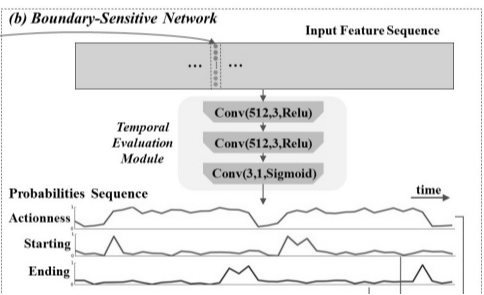
\includegraphics[width=0.8\linewidth]{images/tem2a.png}
    \caption{Temporal Evaluation Module}
    \label{fig:tem}
\end{figure}

\subsection{Proposal generation module}
The main purpose of the proposed generation module is to create proposals for the most important regions of interest in a given video. For this purpose, we followed 2 steps. First, we   identified  time intervals with very high boundary probabilities. These boundaries were then used to define the starting and ending points of the proposals. In the second step, we combine the identified intervals to form complete proposals. We created a Boundary-Sensitive Proposal (BSP) feature for each proposal as shown in figure \ref {fig:gp}. This allowed us to  generate effective proposals for further analysis. 
Initially all  the temporal locations \(t_n\) are recorded, where the staring probabilities \(p^{s}_{t_n}\) are very high. Let say: 
\begin{equation}
    (p^{s}_{t_n}) > 0.9 
\end{equation}
Or starting probability is a peak of that particular region
\begin{equation}
    p_{s,t_n} > p_{s,t_{n-1}} \quad \text{and} \quad p_{s,t_n} > p_{s,t_{n+1}} 
\end{equation}  
These locations are grouped to form a set of candidate starting locations \(B_S = \{ts_i\}_{i=1}^{NS}\) where \(N_S\) represents the total number of candidate starting locations. The same procedure is followed for the generation of the candidate ending location set \(B_E\). Subsequently, we generated temporal regions by combining every starting location with each ending location. As a result, we obtain the candidate proposal set:
\begin{equation}
    \Psi_p = \{\phi_i\}_{i=1}^{N_p}
\end{equation}
where \(N_p\) is the total number of proposals. For each candidate proposal, its center region is denoted by \(r_C\) and its starting and ending regions are denoted by \(r_S\) and \(r_E\) respectively. 
\begin{figure}[h]
    \centering
    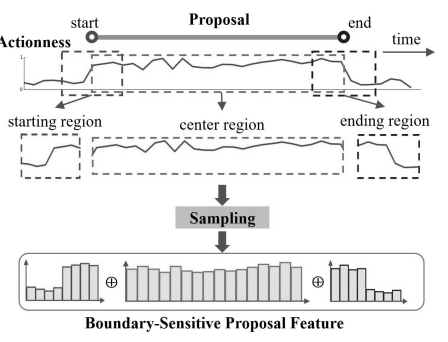
\includegraphics[width=0.7\linewidth]{images/BSPFeature-modified.png}
    \caption{Generating Proposals}
    \label{fig:gp}
\end{figure}
The action sequence within the center region is then represented by \(f^{A}{c}\). It was formed by linearly interpolating the 16 points. On the other hand, the action sequence within the starting and ending regions is represented by \(f^{A}{s}\)  and \(f^{A}{e}\) respectively by linearly interpolating eight points after which a BSP feature is formed.
\begin{equation}
    \mathbf{f_{BSP}} = (f_A^s, f_A^c, f_A^e)
\end{equation}
then every proposal is represented as:
\begin{equation}
    \phi = (ts, te, \mathbf{f_{BSP}})
\end{equation}
\subsection{Proposal evaluation module}
The main objective of the proposed evaluation module was to assign a confidence score to each proposal. This determines whether the actionness instance occurs during the duration. To achieve this, a simple multilayer model was used. It contained a single hidden layer of 512 units. This layer used a Rectified Linear Unit (Relu) activation function. The output layer uses  sigmoid activation to generate the confidence score. This  architecture enables an effective evaluation of action presence within the proposed time as shown in figure \ref {fig:pem}. 


Mathematically,
\begin{equation}
    \phi = (ts, te, \text{pconf}, p_{s_{ts}}, p_{e_{te}})
\end{equation}
where \(p_{s_{ts}}\) and \(p_{e_{te}}\) are the staring and ending probabilities, respectively \(t_s\) and \(t_e\) are the start and end time locations, respectively and \text{pconf} is the confidence score.
\begin{figure}
    \centering
    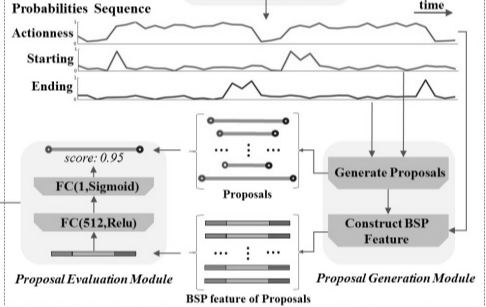
\includegraphics[width=0.7\linewidth]{images/proposalEvaluation-modified.png}
    \caption{Generating Evaluation}
    \label{fig:pem}
\end{figure}


\section{Time series transformer for representation learning}
Time series forecasting is a critical task in various domains, ranging from finance and climate science to the healthcare sector. Traditional methods including the use of Recurrent Neural Networks (RNN) and Convolutional Neural Networks (CNN) face challenges in capturing long-term dependencies in sequential data. On the other hand, transformers keep a connection to all previous timestamps and data, which allows information to propagate over longer sequences. This brings forward the problem of handling large input which is then taken care of by filtering important and unimportant data using the technique of self-attention.
\subsection{Transformer}
Transformer architecture is used under the hood for forecasting methodology, hence it is important to understand how it operates to fully comprehend how forecasting is performed. The transformer is divided into two main components: \textbf{Encoder} and \textbf{Decoder}.
The encoder part as shown in figure \ref{fig:encoder} of the transformer works on the input and it's output is then used in the decoder to process the output. This is done in multiple passes and unlike a feed-forward network, there is only forward propagation and no backward propagation involved in a transformer.
\begin{figure}[h]
    \centering
    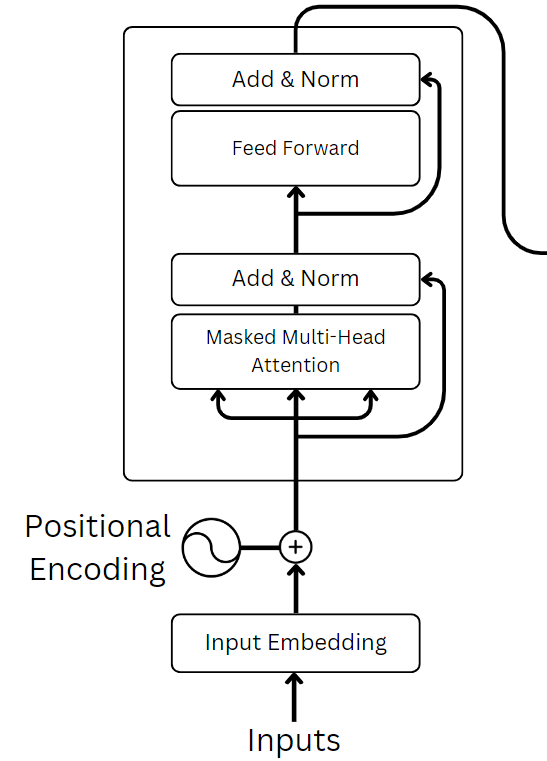
\includegraphics[width=0.35\textwidth]{images/encoder.png}
    \caption{Encoder of a Transformer}
    \label{fig:encoder}
\end{figure}
\subsubsection{Input processing}
The data passed to the transformer is in textual form. A token is not exactly equivalent to a word but for the sake of understanding can be taken as a single word. Each token from the textual data is first assigned an input id which corresponds to the position of a vector in vocabulary of the model, hence an index value. The vocabulary of an encoder are prepared before hand which is known as word embeddings. The word embeddings may be generated using either of the two most popular algorithms namely, Skip-gram and Continuous bag of words (CBOW), used in Word2Vec. The skip-gram predicts the context for a given word and CBOW algorithm predicts the target word given some context. The word embeddings allow the machine to understand complex relations between tokens or words in a higher dimensional space by assigning each word a vector. Here the vector size of 512 signifies the size of the vectors in word embeddings as (1,512). The figure \ref{fig:input} shows how words of a sentence are converted into a number, each corresponding to a word embedding vector.
\begin{figure}[h]
    \centering
    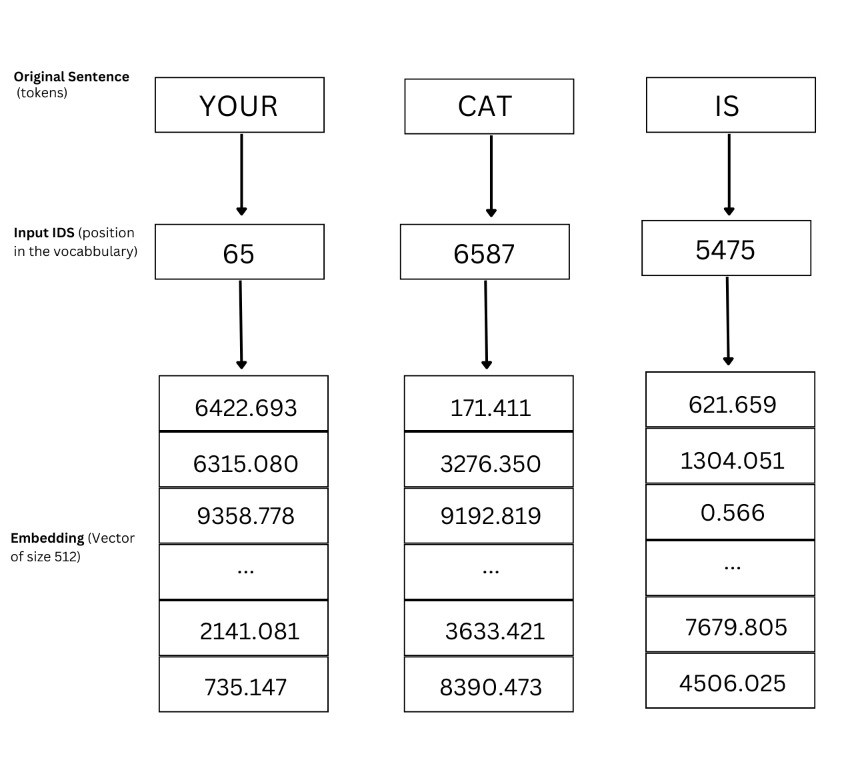
\includegraphics[width=0.65\textwidth]{images/input.jpg}
    \caption{Converting Tokens to Vector Representations}
    \label{fig:input}
\end{figure}
\subsubsection{Positional Encoding}

Once each token is assigned an input id, the vector is fetched from the word embeddings. Each input embedding is then augmented with positional encoding. Positional encoding allows the transformer to understand the sequence of the input tokens. These are calculated using sinusoidal encodings. The figure \ref{fig:sinusoidal} shows how the sinusoidal encodings are generated and the positions are found using three different periods of a sine wave function.
Once the positional encodings are calculated, they are reused and not recomputed. Supposing an example input the sentence "Your Cat Is A Cute Cat". If each word is regarded as a token, then each token receives an input ID that corresponds to the word embedding. The corresponding vectors are fetched and positional encodings are added to them as shown in figure \ref{fig:positional}.
The positional encodings are of the same size as the input. The positional encodings in this example are of the shape (1,512) making it easier to add them up.
\begin{figure}[h]
    \centering
    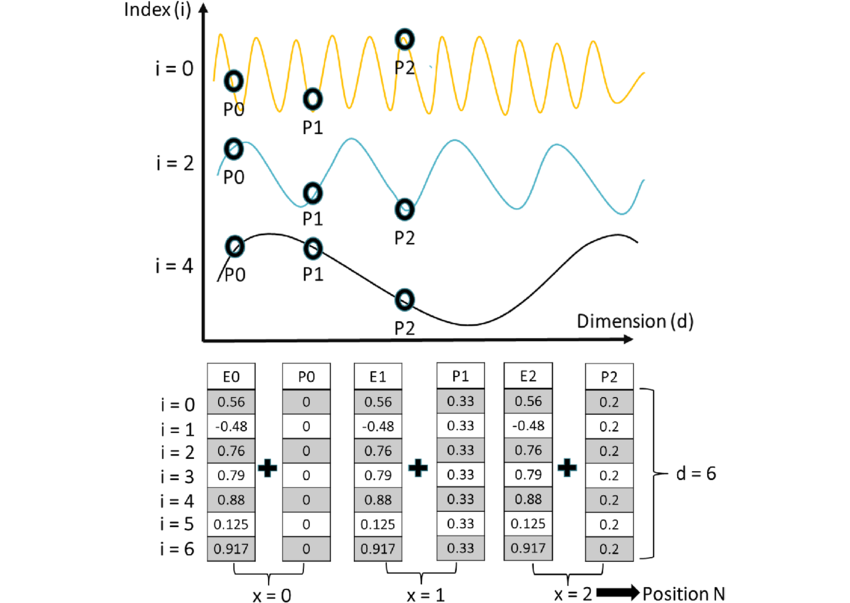
\includegraphics[width=0.65\linewidth]{images/sinusoidal.png}
    \caption{Sinusoidal Positional Encoding}
    \label{fig:sinusoidal}
\end{figure}

\begin{figure}[h]
    \centering
    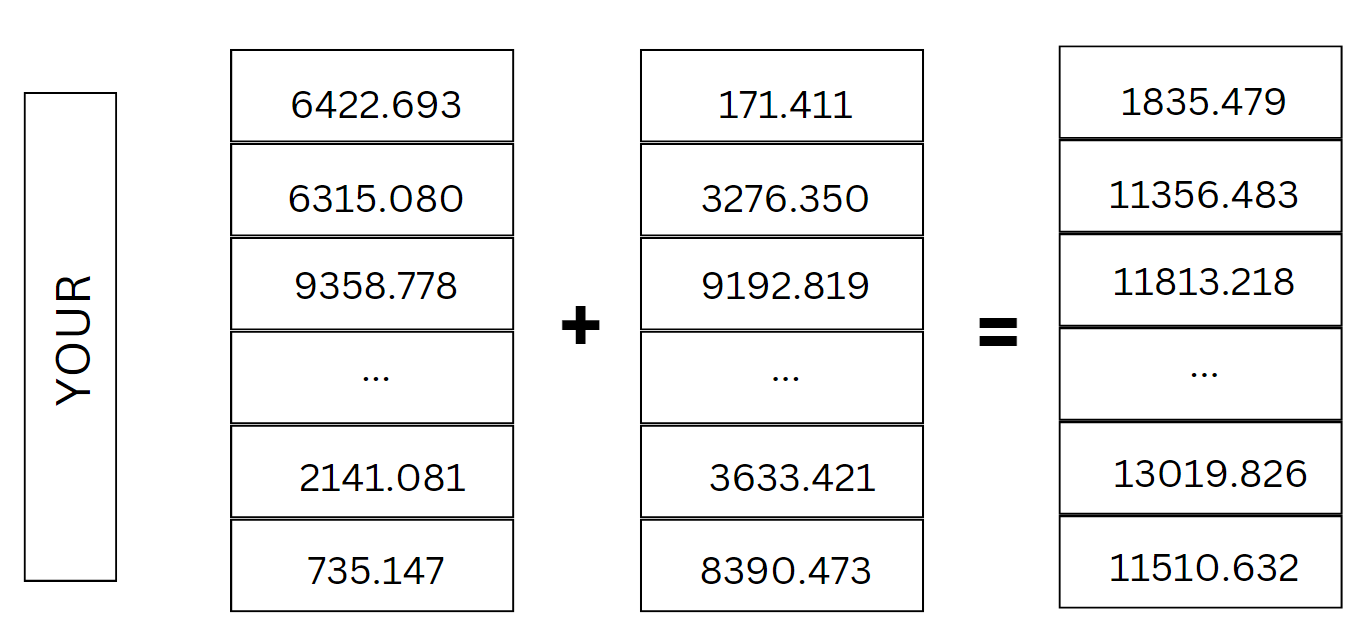
\includegraphics[width=0.75\textwidth]{images/positional.png}
    \caption{Appending Positional Encoding}
    \label{fig:positional}
\end{figure}
\subsubsection{Self-Attention Module}

After augmentation of the input with positional encoding, the vectors are converted into three different projections which are fundamentally three copies. Projection 1 becomes the query, projection 2 becomes the keys, and so projection 3 becomes values. The intuition behind self-attention is to provide each word the required attention from other words. Hence the query is multiplied with the keys to get a matrix. Although additive attention is better at higher values of dk, multiplicative attention is preferred because it computes faster than the additive attention. The multiplicative attention suffers from explosive gradients problem giving extreme values and so a scaling factor of $\sqrt{dk}$ is used. 
\begin{figure}[h]
    \centering
    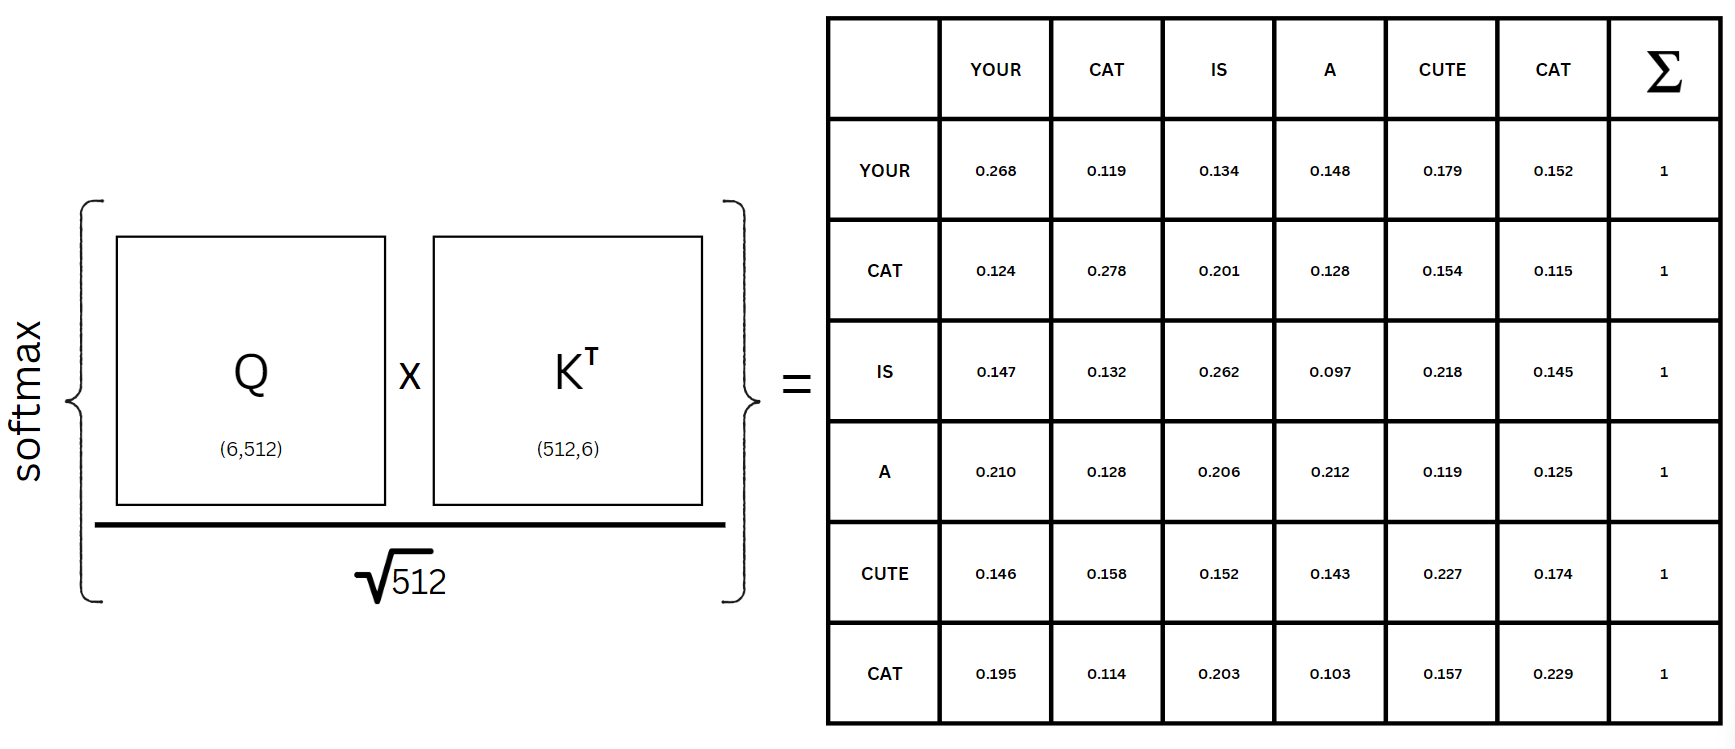
\includegraphics[width=0.75\linewidth]{images/self-attention1.png}
    \caption{Multiplicative Attention}
    \label{fig:self-attention1}
\end{figure}
Conforming to the conventions used in the original paper of transformers by Vaswani et al. 2017, we have mentioned a variable dk. The variable refers to the length of the vector in the word embeddings. Considering the vector shape in the embeddings is of the shape (512,1); then the product of vector of Queries and Keys is divided by the scaling factor of $\sqrt{512}$. 

A product of Values is taken with the output of softmax applied to the previous dot product. The final matrix gives the attention scores. This process as depicted in figures \ref{fig:self-attention1} and \ref{fig:self-attention2} is known as self attention. The input consists of queries and keys of dimension \(d_{k}\), and values of dimension \(d_{v}\). Dot products of the query with all keys, dividing each by the square root of \(d_{k}\), and applying a soft max function to get the weights on the values. The computation of the output matrix is expressed as follows:
\begin{equation}
% \text{Attention}(Q, K, V) = \text{softmax}(\frac{QK^T}{\sqrt{d_k}})V
Attention(Q, K, V ) = softmax\left(\frac{QK^{T}}{\sqrt{d_k}}\right)V
\label{eq:self_attention}
\end{equation}
\begin{figure}[h]
    \centering
    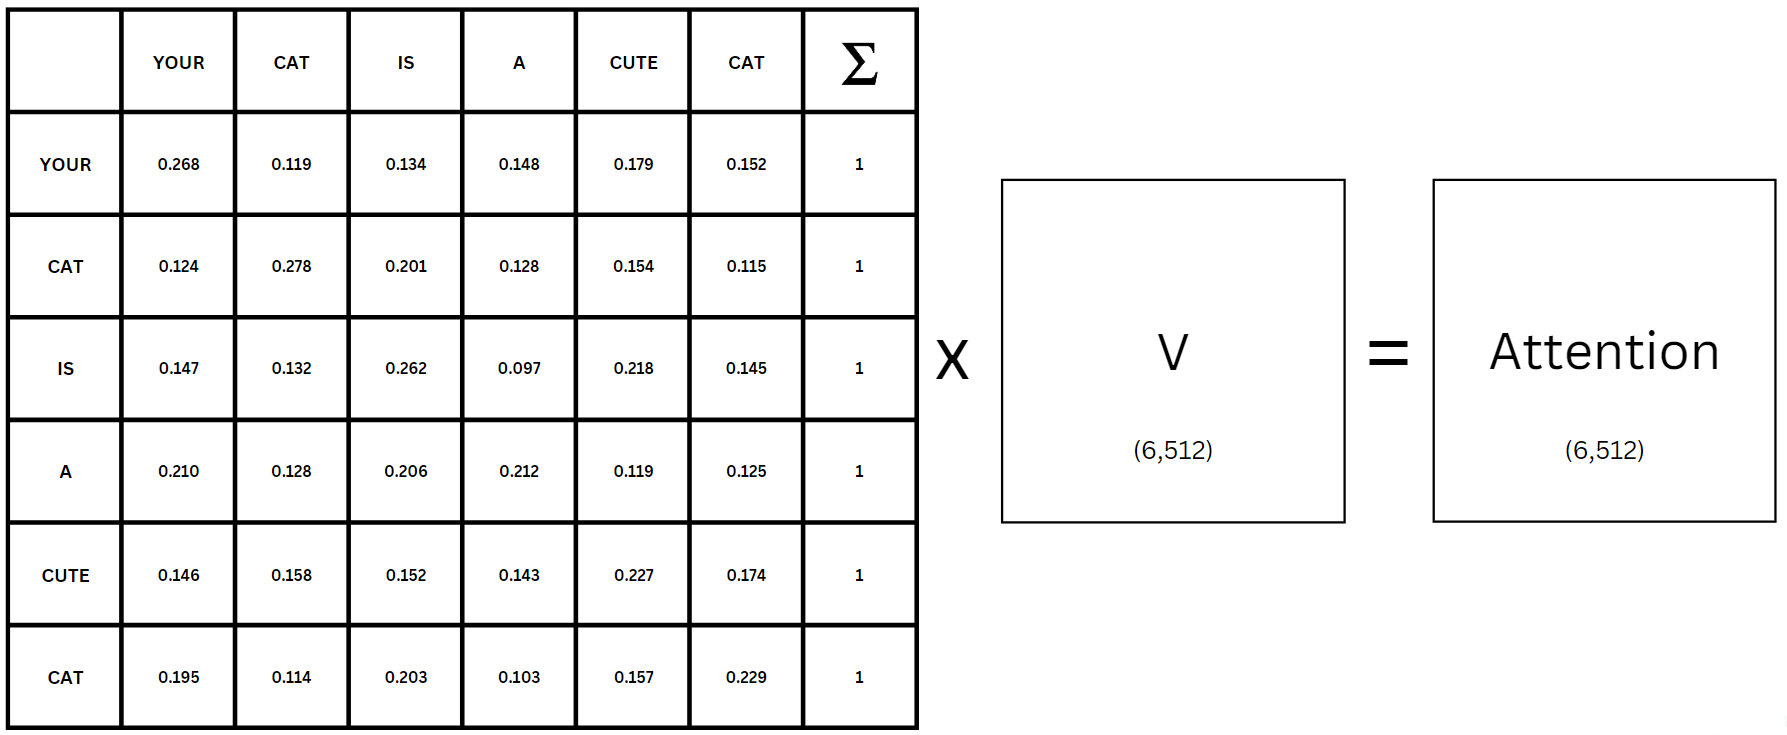
\includegraphics[width=0.75\linewidth]{images/self-attention2.png}
    \caption{Dot Product with Values Gives Attention}
    \label{fig:self-attention2}
\end{figure}
In the example the shape of queries and keys is (6,512). After their dot product, scaling and softmax their shape is (6, 6) which is \((seq, seq)\). A dot product with values of shape (6, 512) returns an attention matrix of shape (6, 512). To make things easier to understand we will be introducing some variables. 6 from the shape of the input is variable \(seq\), hence the number of tokens in the input. \(d_{model}\) is the size of the word embedding which in this case is 512. So the shape of the attention module's output is \((seq, d_{model})\).

\subsubsection{Multi-Head Attention}


To learn different representations, a dot product between each Query, Key and Value is taken with their respective weights. The input matrix is split across the columns according to the number of heads in the self-attention module. The size of the columns now becomes the scaling factor \(d_k\) given by: \[dk = \frac{d_{model}}{h}\]
\begin{figure}[H]
    \centering
    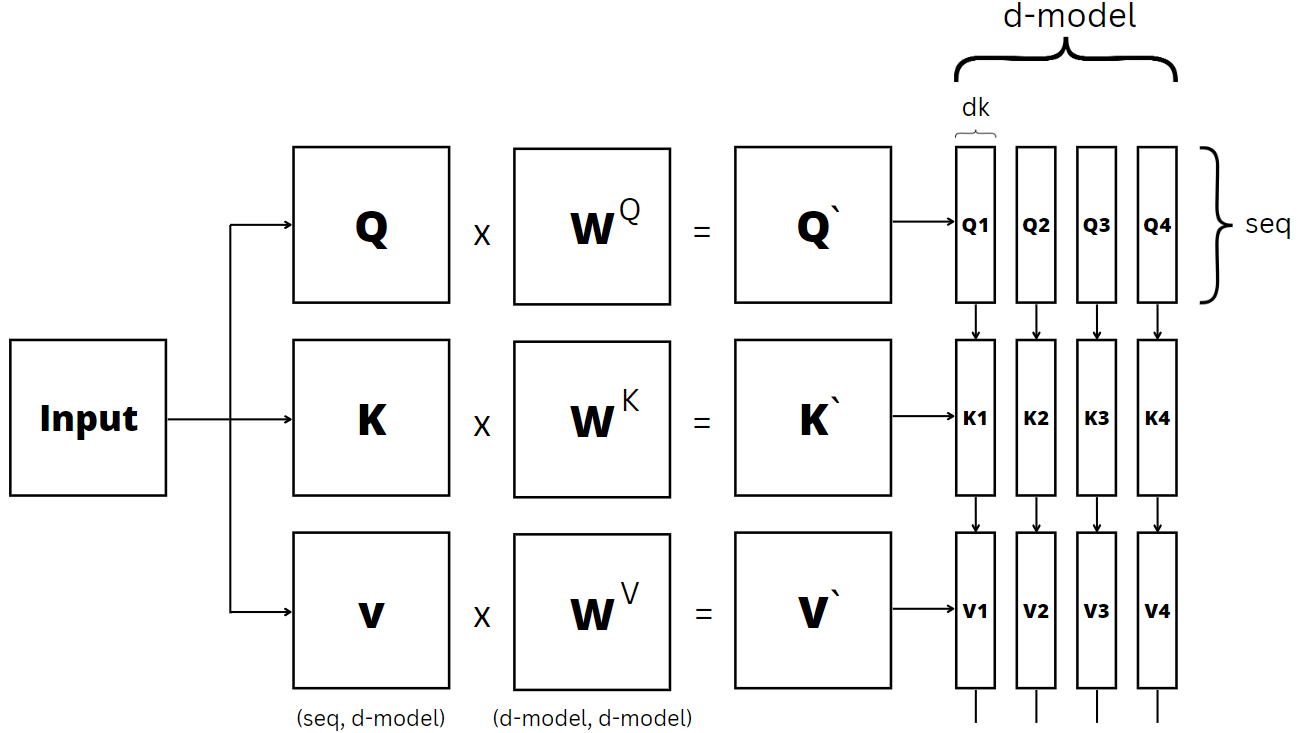
\includegraphics[width=0.75\linewidth]{images/multi1.png}
    \caption{Splitting for Multi-Head Attention}
    \label{fig:multi-head1}
\end{figure}
Then as explained previously, each split is processed by a different attention head. The output of all attention heads are then finally merged and multiplied by weights to give multi-head attention scores. A single head's attention is given as:
\begin{equation}
    head_i = Attention(QW^{Q}_i, KW^{K}_i, VW^{V}_i )
    \label{eq:single-head}
\end{equation}
The Multi-head attention is given as:
\begin{equation}
    MultiHead(Q, K, V) = Concat\left(head_1...head_h\right)W^O
    \label{eq:multi-head}
\end{equation}
Figures \ref{fig:multi-head1}  and \ref{fig:multi-head2} show the complete process involved in multiplicative attention.
\begin{figure}
    \centering
    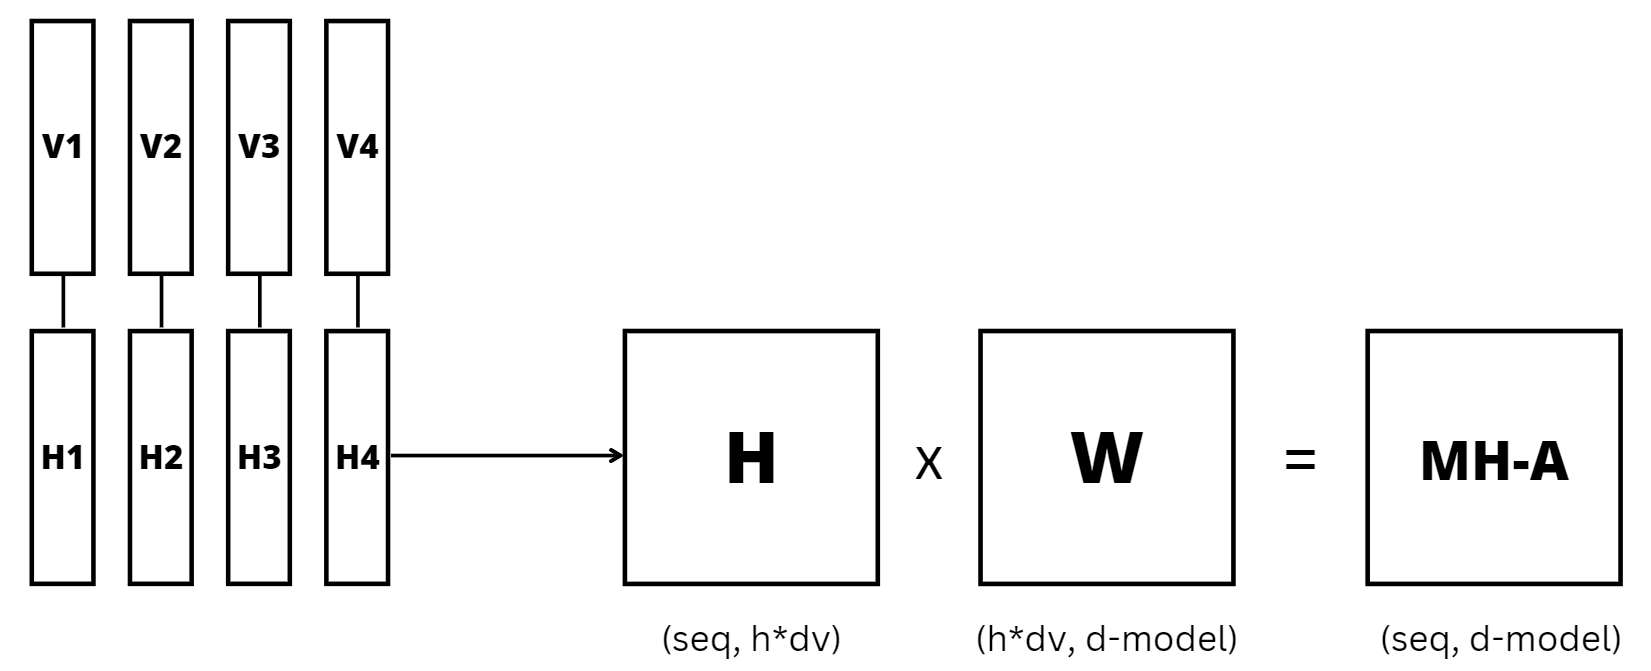
\includegraphics[width=0.75\linewidth]{images/multi-head.png}
    \caption{Output for Multi-Head Attention}
    \label{fig:multi-head2}
\end{figure}
Using the conventions stated before, it can be clearly seen that a dot product is taken for each of the queries, keys and values of shape \((seq, d_{model})\) with their respective weights of shape \((d_{model}, d_{model})\). The dot product gives the output in shape \((seq, d_{model})\) which is then split according to the number of heads \(h\). The shape of \(H\) is defined to be \((seq, h*dv)\) where \(dv\) is the size of values matrix which in this case is equal to \(dk\) but can be kept different. The product with weights of shape \((h*dv, d_{model})\) gives the original shape of \((seq, d_{model})\) which shows \(dv\) can be different from \(dk\).
\subsubsection{Residual Connection}
To keep the original input intact and not lose any important information, an additive attention is used by adding the original input. The output is then batch normalized and passed to the feed-forward neural network. Batch normalization computes the mean and variance across the entire batch for each feature independently normalizing the features within each example based on the statistics of the entire batch. A visual representation of batch normalization is shown in figure \ref{fig:batch-norm}. It is preferred over layer normalization because in time series transformer because it is less affected by the variation in sample lengths found in time series data. The original transformer uses layer normalization to cater to varying input lengths.

\begin{figure}[H]
    \centering
    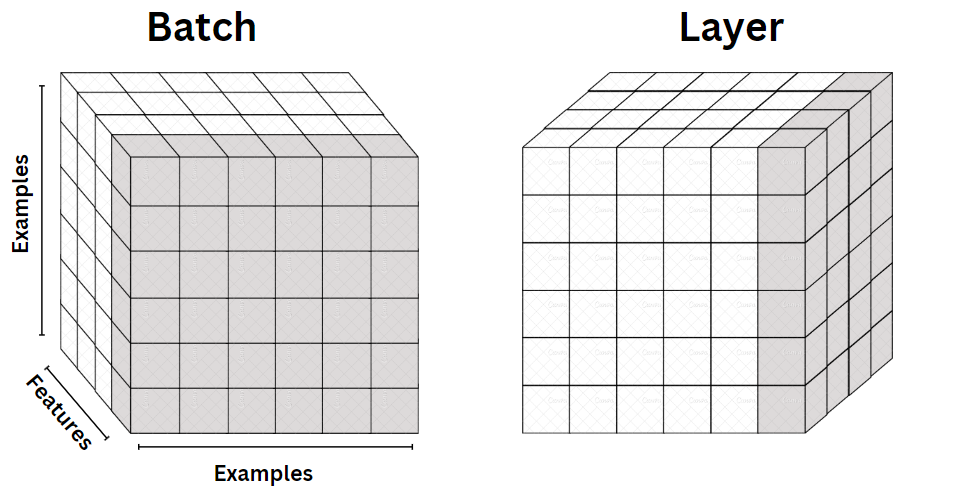
\includegraphics[width=0.7\linewidth]{images/batch-norm.png}
    \caption{Batch Normalization vs Layer Normalization}
    \label{fig:batch-norm}
\end{figure}
\subsubsection{Feed-Forward Neural Network}
The Feed forward neural network uses perceptrons. The perceptrons also known as neurons, compute the dot product of the input with the weights which are initialized using either Xavier Initialization or He Initialization given by: \[W \sim U\left(-\frac{\sqrt{6}}{\sqrt{n_{in}+n_{out}}} ,\frac{\sqrt{6}}{\sqrt{n_{in}+n_{out}}}\right)\]
and
\[W \sim N\left(0 ,\sqrt{\frac{2}{n_{in}}}\right)\]
where U is uniform distribution and N is Normal distribution. An activation function usually Rectified Linear Unit (ReLU) given as: \[ f(x) = \max(0, x) \]
is used on the product and weights are updated using the Adam optimization algorithm. The feed-forward network consists of multiple hidden layers which allow the network to explore the features and relations between tokens in a higher dimensional space. The networks also utilize the concept of auto-encoders where the input is squeezed in a lower dimension and then unsqueezed for effective representation learning. Representation learning refers to learning of underlying structures and relations in the data. Once the representations are learned, they can be used for downstream tasks such as data imputation, regression, classification, and for our case \textbf{forecasting}.

\subsection{Decoder}
The decoder as depicted in figure \ref{fig:decoder} utilizes similar concepts as the encoder. The decoder has two attention modules. The first attention module is called the masked attention module. The input to this module is the output of the transformer's previous pass. In the beginning when there is no output generated, it utilizes a starting terminal character to symbolize the beginning of a sentence. The rest of the output is masked with negative infinity values which prevents the model from knowing the future tokens. This makes the model causal, making it depend on the previously generated token. The masked values when pass through the softmax become 0, hence the name masked attention module. The output of this is used as values and passed along with the output of the encoder which is used as queries and keys in the cross attention module. The output of the cross attention is then passed to feed forward network. The output of the last layer is called logits on which a softmax can be applied but it usually doesnt perform really well. Instead a beam search can be used which selects for each step top B words and evaluate all possible next words for each word selected.
In our use case of forecasting, we will stick to the encoder part because the decoder is more likely used for generative tasks. Using the encoder component only makes the model versatile as it not only helps in regression and classification tasks but can also be used in forecasting.

\begin{figure}[H]
    \centering
    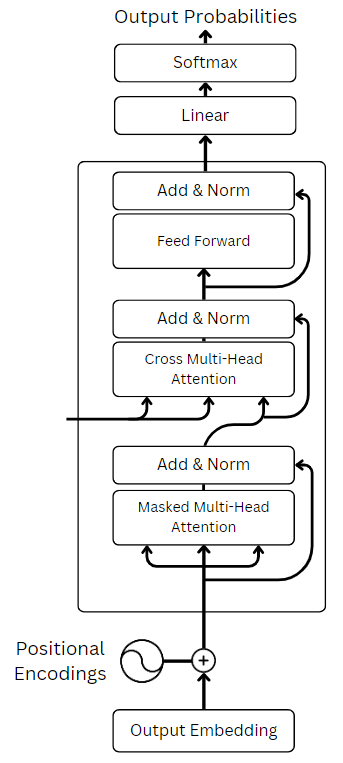
\includegraphics[width=0.35\textwidth]{images/decoder.png}
    \caption{Decoder of a Transformer}
    \label{fig:decoder}
\end{figure}
\subsection{Preprocessing} 
Preprocessing data is a crucial task in time series forecasting. We use simple traditional preprocessing techniques involving scaling to a range of [0,1] or [-1,1], outlier removal, feature engineering, and Input Vector (X) Model Vector (U) Positional Encoding (U') Self Attention Layer Output Vector (Z) standard scaling.
For categorical data, we need to first encode it using Label Encoding i.e., we give a unique numerical value to each category. Once scaling and encoding has been performed, now we bring the sample vectors into the dimensions acceptable by the input. The input format (dimensions) used is an np.ndarray with 3 dimensions i.e., [samples x variables x sequence length]. 
\subsection{Feature Vectors} 
In particular, each training sample  \(X \in R^{w*m}\) where \(w\) is the length of multivariate time series or the number of examples in the input data, and \(m\) is the count of different variables constituting a sequence \(seq\) of \(w\) feature vectors. 
\begin{equation}
    x_{t} \in \mathbb{R}^{m}:X \in \mathbb{R}^{w*m} = [x_{1}, x_{2}, . . ., x_{w}]
    \label{eq:input}
\end{equation}

\subsection{Model Vector (U)}
The figure \ref{fig:base-model} shows the encoder part of the transformer being used in forecasting. The original feature vectors \(x_{t}\) are first normalized by subtracting the mean and dividing by the variance across the training set samples, and then linearly projected onto a \(d\) dimensional vector space, where \(d\) is the dimension of the transformer model sequence element representations, \(d_{model}\): 
\begin{equation}
    u_{t} = W_{p}\cdot x_{t} + b_{p}
    \label{eq:linear projection}
\end{equation}
where \(W_{p} \in \mathbb{R}^{d*m}, b_{p} \in \mathbb{R}^{d}\) are learnable parameters and \(u_{t} \in \mathbb{R}^{d}, t = 0, …, w\)  are the model input vectors, which correspond to the word vectors of the NLP transformer. So a combined form is given by:
\begin{equation}
    U = X \cdot W_{p}^\textit{T} + b_{p}
\end{equation}
These will become the queries, keys, and values of the self-attention layer, after adding the positional encoding and multiplying by the corresponding matrices.
\begin{figure}[h]
    \centering
    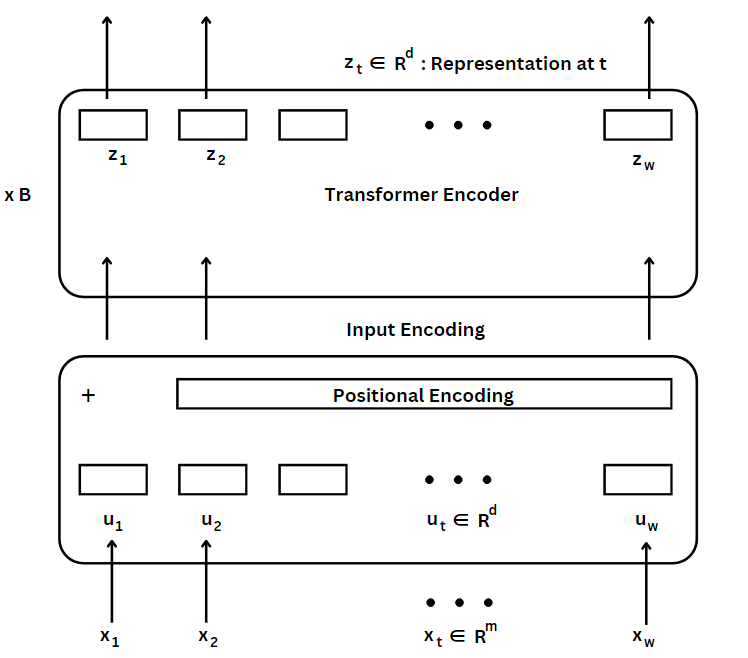
\includegraphics[width=0.7\textwidth]{images/base_tst_model.png}
    \caption{Base Model Representing Transformer}
    \label{fig:base-model}
\end{figure}
\subsection{Positional Encoding}
Before sending the model input vector (U) to the self-attention layer, positional encoding is added to the feed-forward architecture to make it aware of the sequential nature of the time series data. Unlike the original transformer's fixed sinusoidal encodings, fully learnable positional encodings are used. The model’s performance shows that it is independent of the added positional embedding because both the numerical time series information and positional encoding are orthogonal to each other in the vector dimensional space. The positional encodings given by:         \(W_{pos} \in \mathbb{R}^{w*d}\) are added to the input:
\begin{equation}
    U \in \mathbb{R}^{w*d} = [u_1...u_w] : U' = U + W_{pos}
    \label{eq:positional-encoding}
\end{equation}
The dimensions of the input are now \((seq, d_{model})\)
\subsection{Variation in data} 
Time series data may show inconsistency in its length. The shorter samples in the input are padded with arbitrary values and a padding mask adds large negative values to the arbitrary paddings forcing the model to ignore padded positions in softmax and allow parallel processing.

\subsection{Forecasting}
The base model architecture discussed above can be used for the purposes of regression, classification, and forecasting with the following modification: the final representation vectors \(z_{t}\in \mathbb{R}^{d}\) corresponding to all time steps are concatenated into a single vector \(Z \in R^{d*w} = [z1;…;zw]\) , which serves as the input to a linear output layer with parameters \(W_{o} \in \mathbb{R}^{n×(d \cdot w)} , b_{o} \in \mathbb{R}^{n}\)  , where \(n\)  is the number of scalars to be estimated for the regression problem (typically  \(n\)=1), or the number of classes for the classification problem:
\begin{equation}
    \hat{y} =W_{o}Z+b_{o}
\end{equation}
In the case of regression, the loss for a single data sample will simply be the squared error: 
\begin{equation}
    L=|\hat{y}-y|^{2}
\end{equation} 
Where, \(y \in \mathbb{R}^n\)  is the ground truth values. We need to provide different masking patterns to the regression problem that helps in predicting the future values. We may use a sliding window and decide a horizon to predict the future values. 

\section{Experimental Setup}
\subsection{Data Source}
The Data that needs to be collected is obtained from:
\begin{itemize}
    \item Nurse Surveys: The on-duty nurses are asked questions regarding the duties they perform for each patient and how these duties differ for each patient.
    \item Observations recorded from a hospital visit
    \item Research Papers: Using previous research that has been done on electronic nursing systems to extract key information about the nursing workflow.
    \item CCTV Footage: Cameras are setup to collect data which is used to train the model.
\end{itemize}
\subsection{Data Collection Methodology}
The footage is taken from the cameras installed in the wards. Multiple RGB cameras are set up in a ward depending on the size of the ward and the arrangement of the beds. The Cameras captures and detects the patient lying on the bed and the data from the machines next to the patient. To cover all the patients in the ward, cameras facing both sides of the ward will be installed.\\
The footage is cleaned to remove redundant data or parts of the video that are empty. The footage divided into training and testing datasets is used to train and test the AI Model. A clear image of patient vitals monitor is also taken to train the model on different interfaces. 
Surveys are conducted to list down all the details of tasks assigned to a nurse. The patient records maintained by the nurse are studied thoroughly to extract any missed information logged in the records. Previous researches on ENS are used to extract information that is required by a doctor. During the time spent in the nursing ward, observations will be noted about the details involved in nursing. 
Data will be obtained from atleast 4 different hospitals.

\subsection{Data Processing Procedures}
Redundant data and any part of the video that is noisy is removed. The video contains hours of unnecessary stream where there is no one in the ward are trimmed away. Once the necessary processing is done, the video is used for training the AI model.\\
To cater the usage rights and privacy concerns, features are extracted such as patient face. Once the features from this frame are extracted, the video is blurred or have a filter added to it.
The features extracted from this clip are sent down with the video. The video is not sent as a whole because it requires a huge bandwidth so the video is compressed and then sent to the cloud for further processing. The AI Model that has already been trained, utilizes the incoming data and extract the necessary features to classify activities and extract vitals. The model then sends a signal to the dashboard and mobile application alerting the caretakers.\\
The data collected from surveys, interviews, and previous research is used to refine the features of the cross-platform ENS solution.

\subsection{Data Storage and Security}
The video is processed on the desktop at the user’s own end to ensure data integrity. The data extracted from the video is encrypted before being sent to the cloud server to prevent breach of privacy and confidentiality. Once the data is processed in the cloud, it is discarded. The information extracted is stored in an encrypted format. An MOU which has been signed will act as a form of undertaking; that the members working on this project will comply to the data usage rights prescribed by the hospital and will maintain the code of ethics while delivering the necessary output.

% Write in your own chapter title to set the page header % Methodology

% Chapter 5

\chapter{Implementation and Results} % Write in your own chapter title
\label{Chapter5}
\lhead{Chapter 5. \emph{Implementation \& Results}} 
\section{System Requirements}
\lstdefinestyle{python}{
    language=Python,
    basicstyle=\ttfamily\footnotesize, % Use a monospaced font and smaller size
    keywordstyle=\bfseries\color{blue},
    stringstyle=\color{green},
    commentstyle=\color{gray},
    numbers=left, % Line numbers on the left
    numberstyle=\tiny\color{gray},
    stepnumber=1,
    numbersep=10pt,
    frame=single, % Frame around the code block
    breaklines=true, % Enable line breaking
    breakatwhitespace=true, % Only break at whitespace
    tabsize=4, % Set tab size to 4 spaces
    showspaces=false, % Do not display spaces
    showstringspaces=false, % Do not display spaces in strings
    showtabs=false, % Do not display tabs
}
\subsection{Hardware requirements}
As the final product is a software suite, different systems and environments are required to run and coexist. The desktop application requires a minimum of core i5 10th gen processor with 8 GB RAM and 128 GB SSD. Developed in PyQt5, it can be run on Linux, Mac, and Windows OS. The IP cameras used are two mega-pixels (MP) that require network configuration and a readily available internet connection with high bandwidth to send IoT messages and surveillance video to the desktop. The portal is web-based, so it requires no specific operating system to run be it Windows, Linux, or Mac OS. The portal will require a RAM of 8 GB and a processor with specifications i5 8th generation or above. The web server deployed on the cloud service requires a high power multiprocessor to process a large number of requests at a time; thus the distributed computing infrastructure offered by the AWS CloudFormation service is preferable.

\subsection{Software requirements}
The software utilizes multiple third party storage services namely:
\begin{itemize}
    \item \textbf{MMAction2:} Framework used to integrate pre-trained temporal activity localization and recognition models.
    \item \textbf{YoloV5:} Object detection model for tagging and tracking patients.
    \item \textbf{Google-API:} API client used to authenticate the user email address.
    \item \textbf{InfluxDB Cloud 2.0:} Store the patient activity logs.
    \item \textbf{Azure Storage:} Store images and clips of patient when an emergency is detected by the system.
    \item \textbf{PostGreSQL:} Store the user information and the rest of the system database.
\end{itemize}
The system also utilizes \textbf{Stripe's} payment gateway to facilitate online payments. The application backend developed in Python's Django framework was deployed on \textbf{Vercel}.
To communicate IoT messages to the Django web app, a high-bandwidth communication third-party service is integrated, namely, \textbf{Pusher} and \textbf{HiveMqtt}, which are essentially web sockets in nature. They utilize Mqtt and web socket communication protocols for communication. To facilitate the upload and download of pdf files, \textbf{FTP} is used, and \textbf{HTTP} has been used to facilitate client-server communications. Firebase cloud messaging is used to provide push notifications. To allow users to use two-factor authentication (2FA), \textbf{SMTP and POP3} are used to send an email, and \textbf{SMPP} is used for sending an SMS containing a one-time password (OTP). 
\subsection{Deployment}
Developing the desktop app in the PyQt5 framework allows the application to run cross-platform. Using Pyinstaller the application is converted into a single .exe application allowing easy installation. The backend developed in Django is deployed on Vercel in the free tier version. Frontend is deployed on Netlify and cross-origin scripting is ensured with Netlify app as the only allowed origin. The system was tested in a controlled environment within the research lab by integrating an IP Camera of 2 MP and using the project members as test subjects for activity recognition and logging.
\subsection{Training \& Testing of BSN}
\subsection{Dataset}
We used two main datasets for our study: ActivityNet-1.3 and THUMOS14. ActivityNet-1.3 consists of 19,994 videos with 200 action classes. It was used in the ActivityNet Challenges in 2016 and 2017. The dataset was divided into training, validation, and testing sets in a 2:1:1 ratio. THUMOS14 contains 200 and 213 temporally annotated untrimmed videos with 20 action classes in the separate validation and testing sets, respectively. The training set of THUMOS14 was sourced from UCF-101, which contains trimmed videos for action recognition.

\subsection{Training}
We used a two-stream network architecture for visual feature encoding, with BN-Inception serving as the temporal network and ResNet as the spatial network. This architecture was implemented using Caffe and pre-trained on the training set of ActivityNet-1.3. During feature extraction, we set the interval of the snippets to 16 on ActivityNet-1.3 and 5 on THUMOS14.

On ActivityNet-1.3, to account for the limited duration of the videos, we rescaled the feature sequence of each video to a new length of 100 using linear interpolation. The corresponding annotations were  adjusted to fit within the range [0,1]. The temporal and proposal evaluation modules in BSN were implemented using TensorFlow. We trained the temporal evaluation module with a batch size of 16 and  learning rate of 0.001 for 10 epochs, followed by 0.0001 for 10 epochs. The proposed evaluation module was trained using a batch size of 256 and the same learning rate.
\subsubsection{Temporal Evaluation Module}
The temporal evaluation module is designed to assess the probabilities of event start, end, and actionness across all temporal locations within a video. It employs three temporal convolutional layers to extract temporal features, utilizing Rectified Linear Unit (ReLU) activation functions for the first two layers and a Sigmoid activation function for the last layer to generate probability values.
    \begin{lstlisting}[style=python]
    class TEM(torch.nn.Module):
    def __init__(self, opt):
        super(TEM, self).__init__()
        self.feat_dim = opt["tem_feat_dim"]
        self.temporal_dim = opt["temporal_scale"]
        self.batch_size= opt["tem_batch_size"]
        self.c_hidden = opt["tem_hidden_dim"]
        self.tem_best_loss = 10000000
        self.output_dim = 3  
        
        self.conv1 = torch.nn.Conv1d(
        in_channels=self.feat_dim,
        out_channels=self.c_hidden,
        kernel_size=3,
        stride=1,
        padding=1,
        groups=1
        )
        
        self.conv2 = torch.nn.Conv1d(
        in_channels=self.c_hidden,
        out_channels=self.c_hidden,
        kernel_size=3,
        stride=1,
        padding=1,
        groups=1
        )
    
        self.conv3 = torch.nn.Conv1d(
        in_channels=self.c_hidden,
        out_channels=self.output_dim,
        kernel_size=1,stride=1,
        padding=0
        )
        self.reset_params()
        

    @staticmethod
    def weight_init(m):
        if isinstance(m, nn.Conv2d):
            init.xavier_normal(m.weight)
            init.constant(m.bias, 0)

    def reset_params(self):
        for i, m in enumerate(self.modules()):
            self.weight_init(m)

    def forward(self, x):
        x = F.relu(self.conv1(x))
        x = F.relu(self.conv2(x))
        x = torch.sigmoid(0.01*self.conv3(x))
        return x
    \end{lstlisting}

    \subsubsection{Proposed Generation Module}
    
The proposed generation module aims to identify and create proposals for significant regions of interest within a video. It follows a two-step process: first, identifying time intervals with very high boundary probabilities to define starting and ending points; second, combining these intervals to form complete proposals. Each proposal is represented by a Boundary-Sensitive Proposal (BSP) feature, combining actionness sequences from starting, center, and ending regions. Finally, each proposal is represented by its starting and ending points along with its BSP feature.
\begin{lstlisting}[style=python]

def generateProposals(opt,video_list,video_dict):
    tscale = opt["temporal_scale"]    
    tgap = 1./tscale
    peak_thres= opt["pgm_threshold"]

    for video_name in video_list:
        tdf=pandas.read_csv("./output/TEM_results/"+video_name+".csv")
        start_scores=tdf.start.values[:]
        end_scores=tdf.end.values[:]        
        max_start = max(start_scores)
        max_end = max(end_scores)
        
        start_bins=numpy.zeros(len(start_scores))
        start_bins[[0,-1]]=1
        for idx in range(1,tscale-1):
            if start_scores[idx]>start_scores[idx+1] 
            and
            start_scores[idx]>start_scores[idx-1]:
                start_bins[idx]=1
            elif start_scores[idx]>(peak_thres*max_start):
                start_bins[idx]=1
                    
        end_bins=numpy.zeros(len(end_scores))
        end_bins[[0,-1]]=1
        for idx in range(1,tscale-1):
            if end_scores[idx]>end_scores[idx+1] 
            and
            end_scores[idx]>end_scores[idx-1]:
                end_bins[idx]=1
            elif end_scores[idx]>(peak_thres*max_end):
                end_bins[idx]=1
        
        xmin_list=[]
        xmin_score_list=[]
        xmax_list=[]
        xmax_score_list=[]
        for j in range(tscale):
            if start_bins[j]==1:
                xmin_list.append(tgap/2+tgap*j)
                xmin_score_list.append(start_scores[j])
            if end_bins[j]==1:
                xmax_list.append(tgap/2+tgap*j)
                xmax_score_list.append(end_scores[j])
                
        new_props=[]
        for ii in range(len(xmax_list)):
            tmp_xmax=xmax_list[ii]
            tmp_xmax_score=xmax_score_list[ii]
            
            for ij in range(len(xmin_list)):
                tmp_xmin=xmin_list[ij]
                tmp_xmin_score=xmin_score_list[ij]
                if tmp_xmin>=tmp_xmax:
                    break
                new_props.append(
                [
                tmp_xmin,tmp_xmax,
                tmp_xmin_score,
                tmp_xmax_score
                ]
                )
        new_props=numpy.stack(new_props)
        col_name=["xmin","xmax","xmin_score","xmax_score"]
        new_df=pandas.DataFrame(new_props,columns=col_name)  
        new_df["score"]=new_df.xmin_score*new_df.xmax_score
        new_df=new_df.sort_values(by="score",ascending=False)
        
        video_info=video_dict[video_name]
        video_frame=video_info['duration_frame']
        video_second=video_info['duration_second']
        feature_frame=video_info['feature_frame']
        corrected_second=float(feature_frame)/video_frame*video_second
        
        try:
            gt_xmins=[]
            gt_xmaxs=[]
            for idx in range(len(video_info["annotations"])):
                gt_xmins.append(
                video_info["annotations"][idx]["segment"][0]
                /
                corrected_second
                )
                gt_xmaxs.append(
                video_info["annotations"][idx]["segment"][1]
                /
                corrected_second
                )
            new_iou_list=[]
            for j in range(len(new_df)):
                tmp_new_iou=max(
                iou_with_anchors(
                new_df.xmin.values[j],
                new_df.xmax.values[j],
                gt_xmins,
                gt_xmaxs)
                )
                new_iou_list.append(tmp_new_iou)
                
            new_ioa_list=[]
            for j in range(len(new_df)):
                tmp_new_ioa=max(
                ioa_with_anchors(
                new_df.xmin.values[j]
                ,new_df.xmax.values[j],
                gt_xmins,gt_xmaxs)
                )
                new_ioa_list.append(tmp_new_ioa)
            new_df["match_iou"]=new_iou_list
            new_df["match_ioa"]=new_ioa_list
        except:
            pass
        new_df.to_csv("./output/PGM_proposals/"+video_name+".csv",index=False)
    \end{lstlisting}
\subsubsection{Proposal evaluation module}
    
The proposed evaluation module assigns confidence scores to each proposal, determining the likelihood of action occurrence within its duration. It employs a simple multilayer model with a hidden layer of 512 units using Rectified Linear Unit (ReLU) activation, and a sigmoid activation for the output layer to generate the confidence score. Each proposal is represented by its start and end time locations, along with starting and ending probabilities, and the confidence score.

\begin{lstlisting}[style=python]
class PEM(torch.nn.Module):
    
    def __init__(self,opt):
        super(PEM, self).__init__()
        self.feat_dim = opt["pem_feat_dim"]
        self.batch_size = opt["pem_batch_size"]
        self.hidden_dim = opt["pem_hidden_dim"]
        self.u_ratio_m = opt["pem_u_ratio_m"]
        self.u_ratio_l = opt["pem_u_ratio_l"]
        self.output_dim = 1
        self.pem_best_loss = 1000000
        
        self.fc1 = torch.nn.Linear(
        in_features=self.feat_dim,
        out_features=self.hidden_dim,
        bias =True
        )
        
        self.fc2 = torch.nn.Linear(
        in_features=self.hidden_dim,
        out_features=self.output_dim,
        bias =True
        )
        self.reset_params()

    @staticmethod
    def weight_init(m):
        if isinstance(m, nn.Conv2d):
            init.xavier_uniform_(m.weight)
            #init.xavier_normal(m.weight)
            init.constant(m.bias, 0)

    def reset_params(self):
        for i, m in enumerate(self.modules()):
            self.weight_init(m)

    def forward(self, x):
        x = F.relu(0.1*self.fc1(x))
        x = torch.sigmoid(0.1*self.fc2(x))
        return x
    \end{lstlisting}
\subsection{Result}
A crucial aspect of proposal generation methods is their ability to generate proposals for unseen action classes. To assess this, we selected two distinct action subsets from ActivityNet-1.3: "Sports, Exercise, and Recreation" and "Socializing, Relaxing, and Leisure" as seen and unseen subsets, respectively. The seen subset comprised 87 action classes with 4455 training and 2198 validation videos, while the unseen subset consisted of 38 action classes with 1903 training and 896 validation videos. The result were as follows:

\begin{figure}[H]
    \centering
    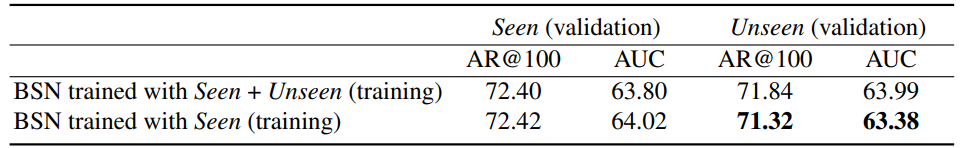
\includegraphics[width=\linewidth]{images/traing.png}
    \caption{Generalization Evaluation of BSN on ActivityNet-1.3. Seen Subset: “Sports, Exercise, and Recreation”; Unseen Subset: “Socializing, Relaxing, and Leisure”}
    \label{fig:BSN Evaluation}
\end{figure}
In our evaluation on the ActivityNet proposal task, our model achieved promising results. The Area Under the AR vs AN curve reached 67.42\%. For individual performance metrics, the model achieved an AR@1 of 32.93\%, AR@5 of 47.72\%, AR@10 of 55.59\%, and AR@100 of 75.12\%. These results indicate the effectiveness of the model in generating proposals for action recognition tasks.

\begin{figure}[H]
    \centering
    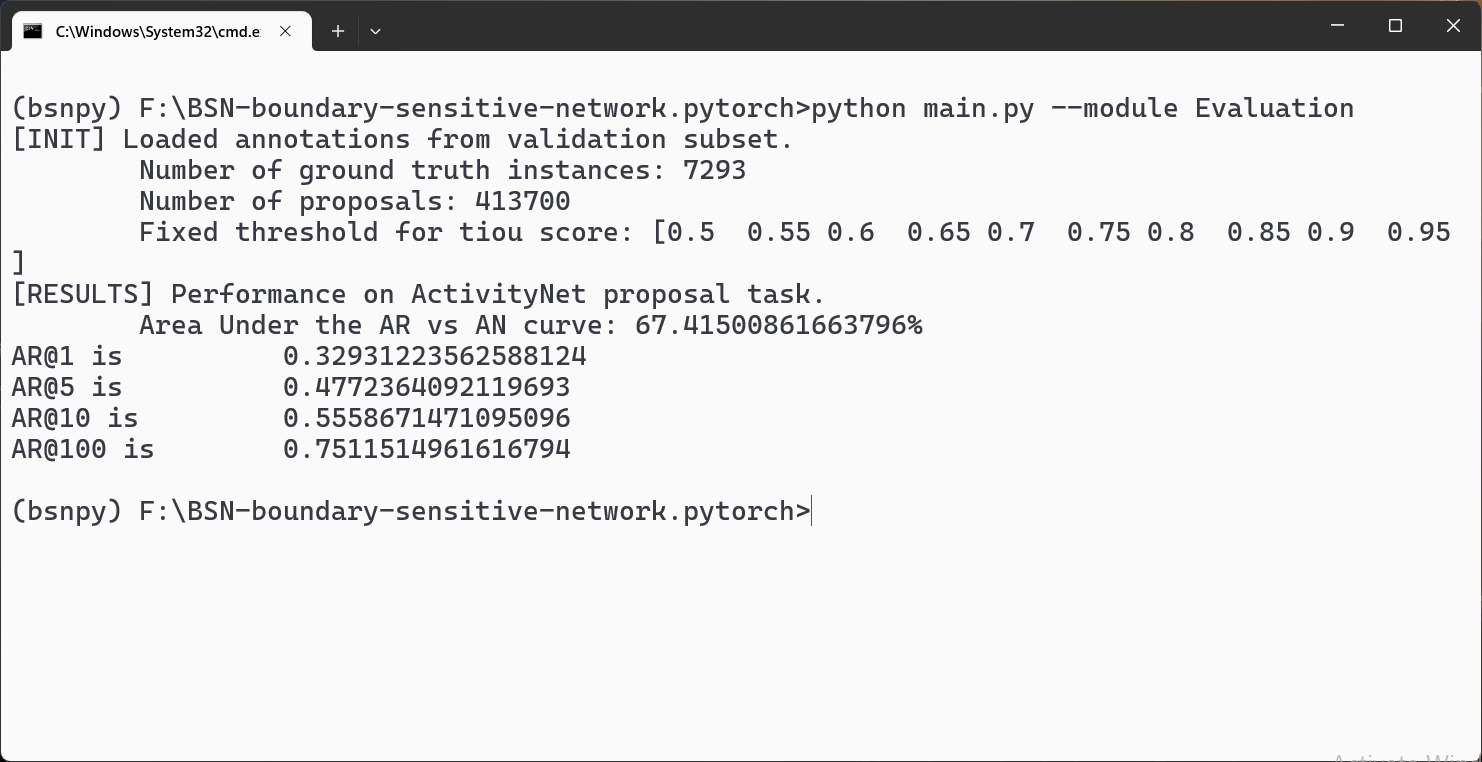
\includegraphics[width=0.8\linewidth]{images/result1.png}
    \caption{Model Accuracy}
    \label{fig:result CMD}
\end{figure}
\begin{figure}[H]
    \centering
    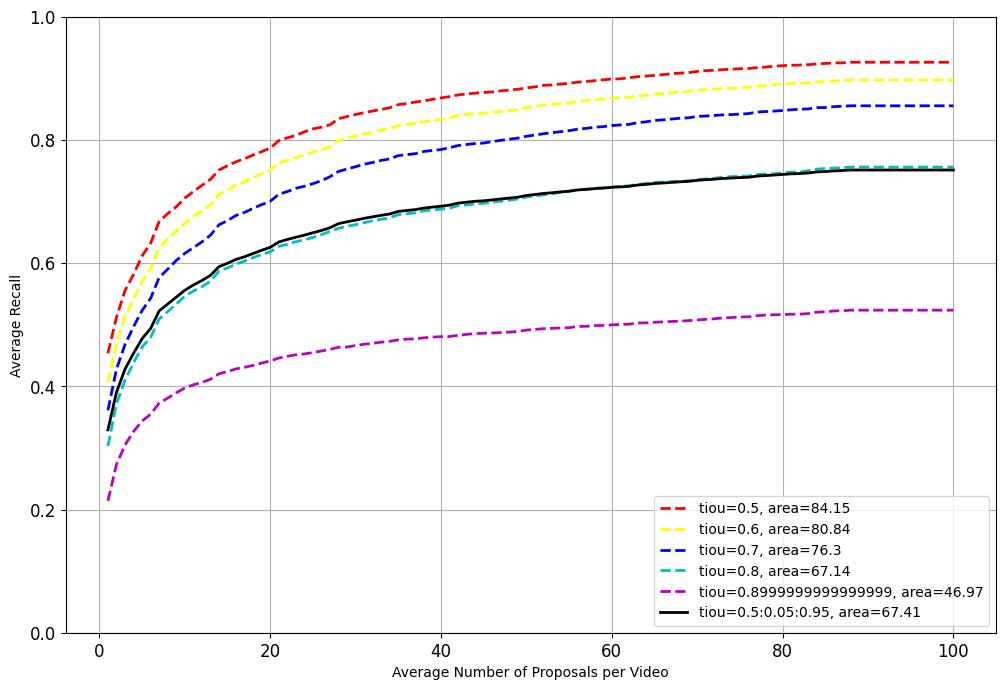
\includegraphics[width=0.7\linewidth]{images/result2.jpg}
    \caption{Relationship Between Average Recall and Proposal per Video}
    \label{fig:BSN Results}
\end{figure}

\subsection{Implementation \& Results of Transformer}
\subsubsection{Dataset}
To train the TST Plus model we use the Balanced Toyota Smarthome Untrimmed (TSU) dataset with 31 activities. To get the annotated data set we use the Balanced Toyota Smarthome repository \cite{btsu}. We save the annotated data in a separate file. The file is such that it contains 351 training data and 185 validation data. Each item of the annotated training and validation data consists of the video name, one hot encoding, number of frames, and the duration of the activity. The following code outputs the data shape and format that is loaded into the google colab notebook as shown in figure  \ref{fig:training-data tst}.
\begin{lstlisting} [style=python]
train_data = content['train']
validation_data = content['val']
combined_data = []
for value in train_data:
  print("Video Name: ",value[0],"--One Hot: ",value[1].shape,"--Frames: ",value[2],"--seconds: ",value[1].shape[0],value[2]//16)
  for val in value[1]:
    combined_data.append(val)
np_combined = np.array(combined_data)
np_combined.shape
\end{lstlisting}
\begin{figure}[h]
    \centering
    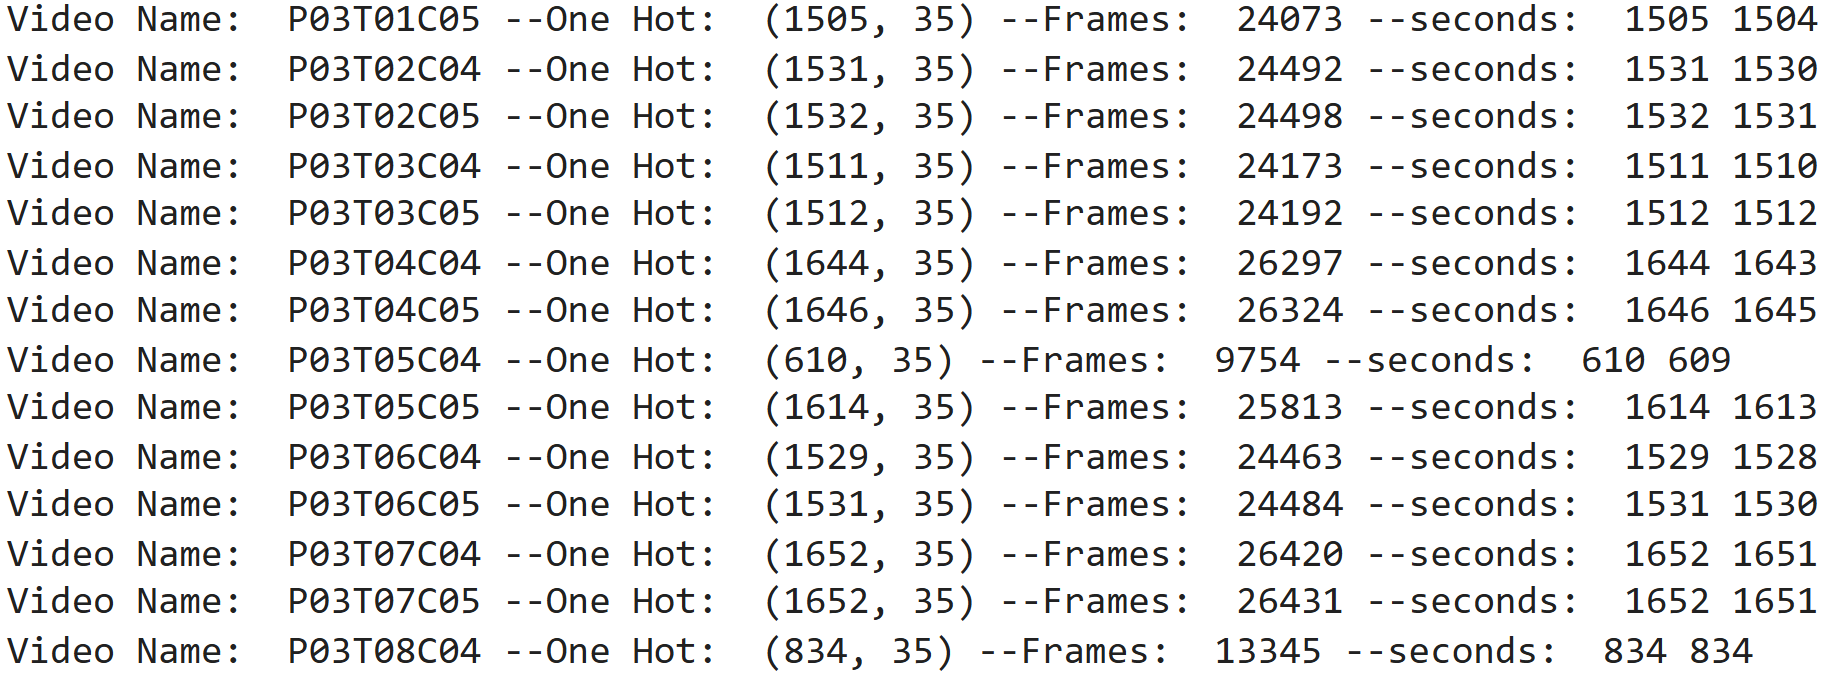
\includegraphics[width=0.7\linewidth]{images/trainingDataTST.png}
    \caption{Annotated Data}
    \label{fig:training-data tst}
\end{figure}

The training and validation data is further passed to the TST Plus model. We set the hyper parameters and number of iterations for training. The hyperparameters used in the training are:
\begin{enumerate}
    \item Learning rate: 1e-3
    \item Sliding window size: 32
    \item Horizon: 5
\end{enumerate}
\subsubsection{Model Training}
We use the TSAI \cite{tsai} library to forecast the activities of the patients. TSAI comprises of many forecasting models but we use the TST Plus to forecast the activities. The code for the TST Plus model's training is as shown below. Utilizing the pre-existing library provided by TSAI, the model is trained. Our input is the tuning of the hyper-parameters to give the most optimal forecasting accuracy
\begin{lstlisting}[style=python] 
from sklearn.metrics import accuracy_score , mean_squared_error , confusion_matrix
def activity_forecasting_model_training(forecasting_data , model, learning_rate , sliding_window_size , horizon , validation_size ,number_of_iterations):
  X, y = SlidingWindow(sliding_window_size, horizon=horizon)(forecasting_data)

  splits = TimeSplitter(validation_size, fcst_horizon=horizon)(y)

  tfms = [None, TSForecasting()]
  batch_tfms = TSStandardize()
  fcst = TSForecaster(X, y, path='models', splits = splits,tfms=tfms, batch_tfms=batch_tfms, bs=512, arch=model, metrics=mae )
  fcst.fit_one_cycle(number_of_iterations, learning_rate)

  raw_preds, target, preds = fcst.get_X_preds(X[splits[1]], y[splits[1]])
  return preds , target , raw_preds
\end{lstlisting}
The Model training output is shown in figures \ref{fig:training-split} and \ref{fig:training-model}. 
\begin{figure}[H]
    \centering
    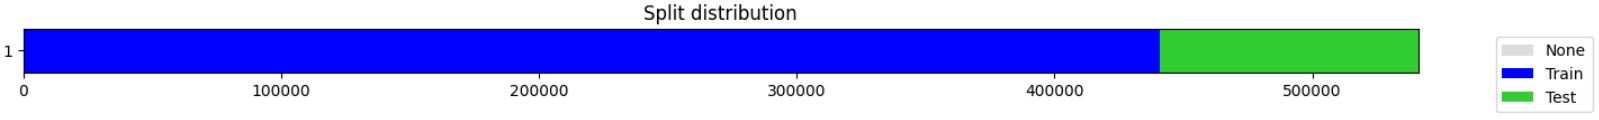
\includegraphics[width=\linewidth]{images/training split.png}
    \caption{Training Split for TST Plus Model}
    \label{fig:training-split}
\end{figure}
\begin{figure}[H]
    \centering
    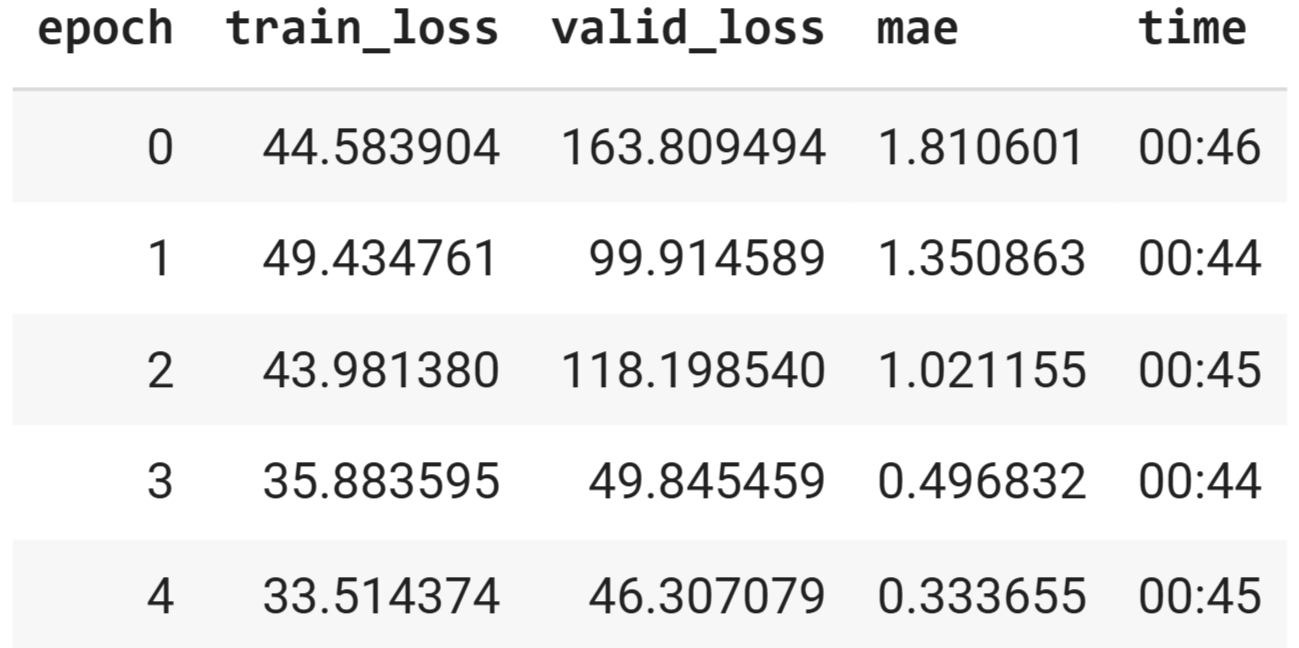
\includegraphics[width=0.7\linewidth]{images/training model.png}
    \caption{Training Results}
    \label{fig:training-model}
\end{figure}



\subsubsection{Results}
Due to limited resources we were not able to fully explore the potential of the TST forecaster as the colab session would break and crash. We were limited to running only a few iterations with a limited window size and a limited horizon size. After the training is completed we see that the Mean Absolute Error (MAE) is 0.33 as shown in Figure \ref{fig:training-model}. We further calculate the accuracy of our model using the code as in figure \ref{fig:tst accuracy} amounting to a staggering 39.88\% considering the limited training.
\begin{figure}[H]
    \centering
    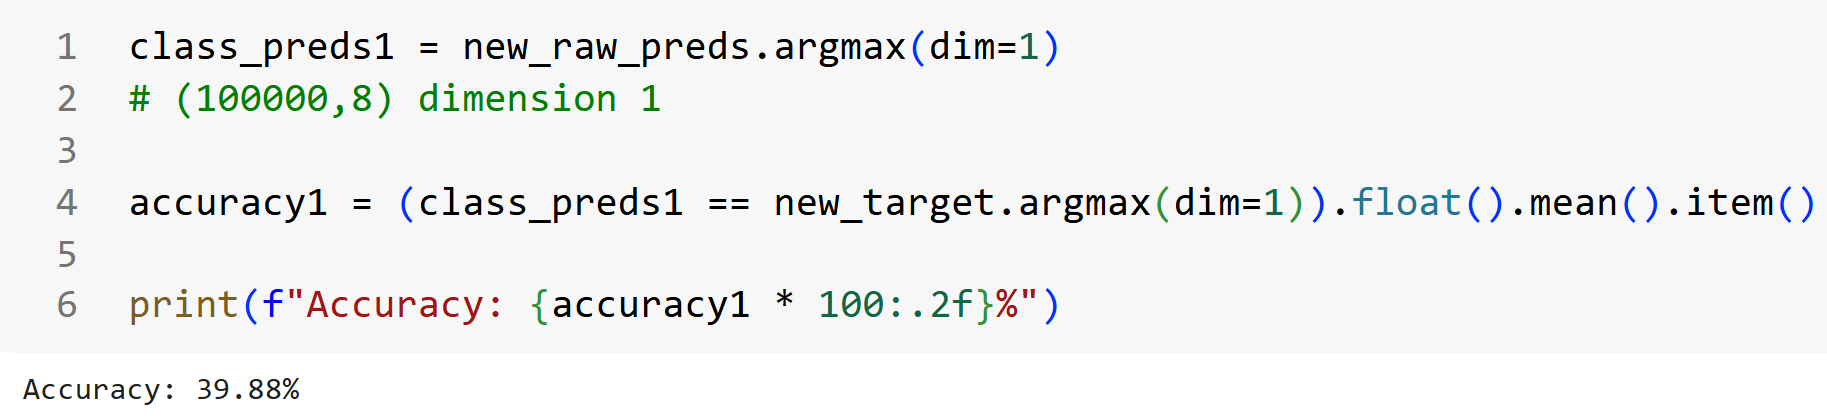
\includegraphics[width=1\linewidth]{images/trainingResultTST.png}
    \caption{Accuracy of TST Plus Model After Training it on Balanced Toyota Smarthome Untrimmed Dataset}
    \label{fig:tst accuracy}
\end{figure}
 % Implementation and Results

% Chapter 4

\chapter{Nursing Care Dashboard (NCD)} % Write in your chapter title
\label{Chapter6}
\lhead{Chapter 6. \emph{Nursing Care Dashboard}} 
\section{NCD Perspective}
In this chapter, we provide a holistic perspective on the product highlighting its scope, functions, user classes, and architectural design to explain the vision and impact of the project within the healthcare domain.
The scope of ENS is focused on addressing the unique healthcare needs of elderly patients through a comprehensive set of functions. These functions encompass intelligent reporting, real-time monitoring, workflow integration, and AI-assisted insights. ENS seeks to enhance patient care, streamline workflows, reduce nurse burnout, and empower nurses and doctors with actionable insights. 
At the core of ENS is a user-centric approach to cater to the needs of nurses in the healthcare ecosystem. By prioritizing nurses, ENS aims to optimize user experience, facilitate collaboration, and improve patient outcomes. This emphasis on user classes and characteristics ensures that ENS is tailored to meet the specific requirements and preferences of the nurses.
The architectural framework of ENS highlights its technical sophistication and scalability. It uses different parts like cameras, AI in the cloud, and a website. This setup makes ENS a smart way to improve healthcare. It lets us easily collect, study, and share data. This lays the foundation for real-time patient monitoring and decision support. 
Beyond its immediate functionalities, ENS holds profound implications for the future of healthcare delivery.  ENS aims to revolutionize patient care by empowering healthcare professionals and enhancing the overall quality and efficiency of healthcare services. As we embark on this journey, we envision ENR as a catalyst for transformative change in the healthcare landscape, driving toward a future where nurses perform up to their potential and every patient receives personalized, proactive, and effective care.
 
\section{NCD Scope}
The scope of the product is defined in the following particulars:
\begin{itemize}
    \item The initial focus is on elderly patients
    \item Assist nursing care workflow
    \item Assist the doctor with decision and diagnosis
    \item Fixed number of activities and behaviors.
    \item The product will not detect abnormal activities.
    \item The product will be offered in home settings as well as in hospital settings
    \item The product will log vital signs with minimum human intervention.
    \item The product will alert the user in case of any irregularity in vital signs.
    \item Clients will be offered different payment and service plans.
\end{itemize}
\section{User Classes and Characteristics}
The most important users of the system are listed below in order of decreasing priority:
\begin{itemize}
    \item \textbf{Admin/Buyer:} For our business model the buyer of our product is the most important who will have the exclusive rights to maintain the whole system and the users associated with it.
    \item \textbf{Nurse:} The major user of the system around whom the whole system revolves. Some of their tasks will be automated while others digitized to remove anomalies produced in manual paperwork and management.
    \item \textbf{Doctor:} The decision maker. The doctor receives complete information about the patient from the nurse through the application. They can view the patient status, analyze near real-time data remotely, and make an informed decisions.
    \item \textbf{Caretaker:} The tertiary user of the system will only be able to view the patient status unless they are also the owner of the system.

\end{itemize}

Although the doctor makes the decisions, they rank below in priority as the system is aimed at assisting the nurses first. The Doctors' decision becomes secondary in a situation where there is no proper care being provided to the patient; where there is no proper patient information collection which is to be communicated to a doctor for decision making.
The caretakers need not have a screen but it is necessary to provide the caretakers of a patient the complete access to near real-time updates and status of their patient. This will allow them to rest easy in their home instead of staying in the hospitals for a long duration. It will also reduce the cynical attitude and delayed adoption of AI technology resulting in delayed technological advancements.
\pagebreak
\subsection{Database Diagram}
The Figure \ref{fig:db-diagram} shows the complete database that was utilized in the development of the prototype. The tables have been normalized to 3NF. Practically the patient logs are being kept in the InfluxDB Cloud to keep all the records while the rest of the database is in a single PostGreSql database deployed on NeonDB Cloud Serverless service.
\begin{figure}[h]
    \centering
    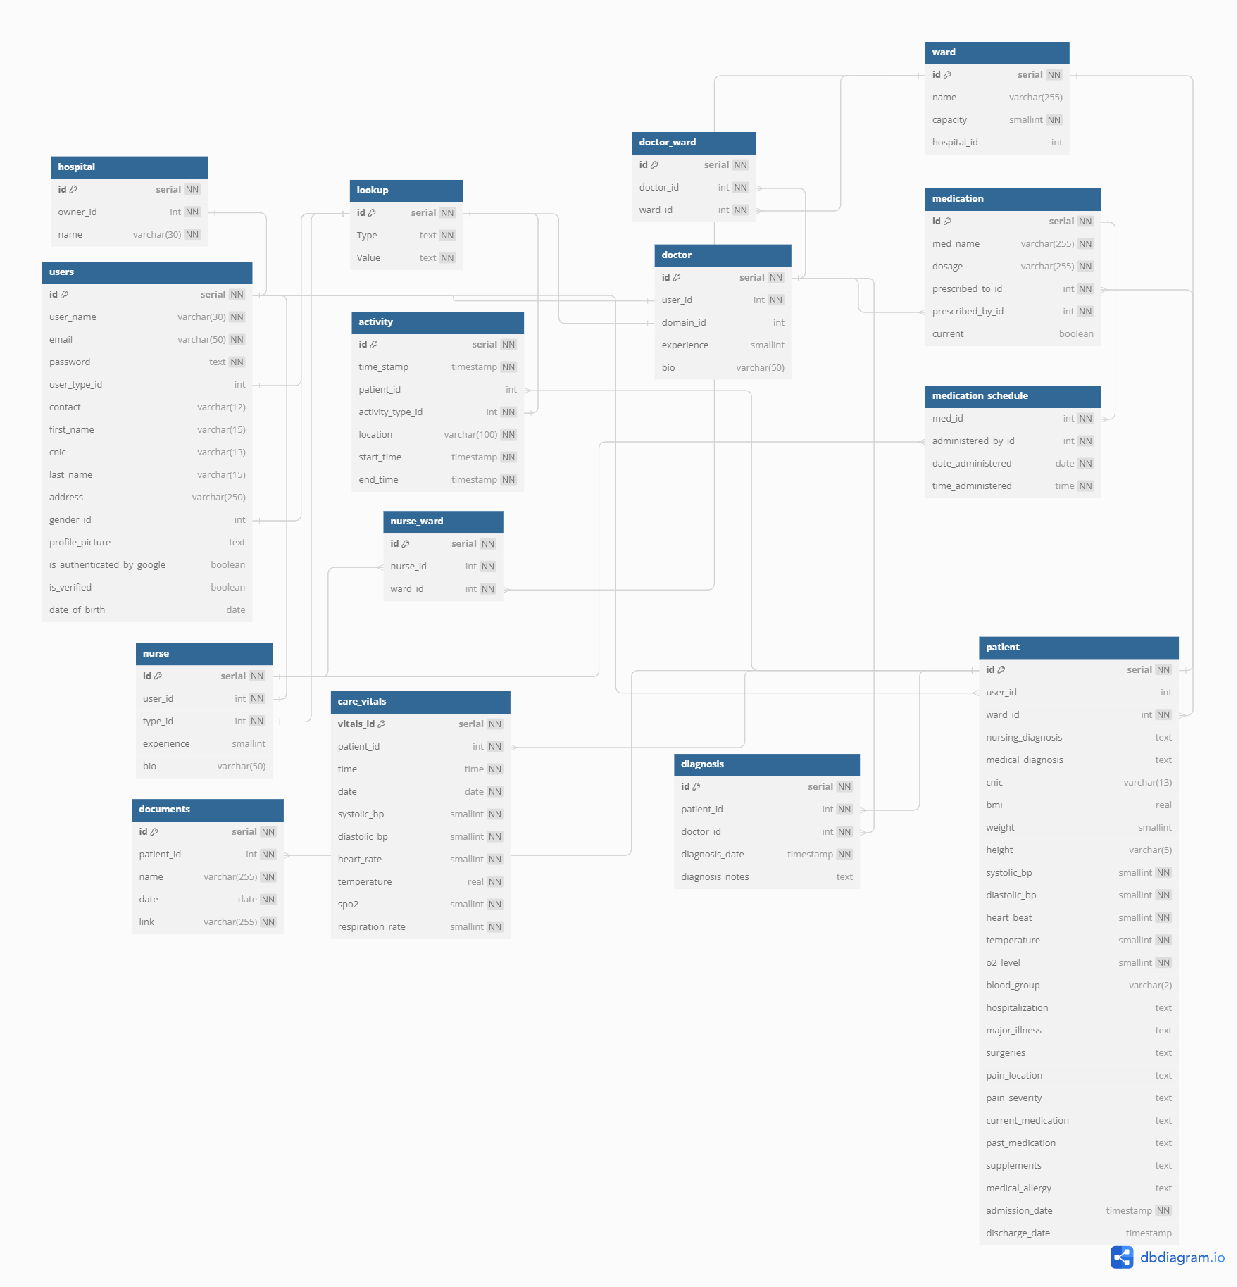
\includegraphics[width=\textwidth]{images/db.pdf}
    \caption{System Database Diagram}
    \label{fig:db-diagram}
\end{figure}
\section{Modules}
\subsection{Acquisition and Account}
\subsubsection{Purpose}
Authenticate users based on their credentials to allow only authorized users to view and manipulate sensitive patient records. It is also to allow authorized users to maintain and update their profiles as needed. Allow new payments to be processed and allow only authorized personnel to use the software in an attempt to curb software piracy. Moreover, to allow customers and potential clients to contact us. It is also aimed at improving the product based on feedback.
\subsubsection{Sub Modules}
\begin{enumerate}
    \item User Registration
    \item Account Management
    \item Payment Management
    \item Technical Support and Contact
\end{enumerate}
\subsubsection{Functional Requirements}
\begin{enumerate}
    \item      Hospital admin can sign up with a Google account or sign up with any email.
    \item Users are only allowed to login if they have been verified through email.
    \item Once verified they need to select a payment plan to proceed using the web portal.
    \item Hospital admin can add or remove doctors, nurses and patients.
    \item The users added by the hospital will be associated with the hospital.
    \item Hospital may choose existing doctor as well from a list of doctor accounts that are previously registered with the portal instead of making a duplicate account.
    \item The credentials will be auto-generated by the admin.
    \item The user may change their password after logging in successfully.
    \item Each user added by admin will be verified on login through an OTP sent to their mobile number.
    \item Users can view all payment plans offered.
    \item Users can select any of the payment plans of their choice.
    \item Users can make payment via an online payment gateway.
    \item Once payment is verified the user will receive a downloadable desktop application along with a unique product key.
    \item The user will be able to use the application if and only if they enter a valid product key.
    \item The user can renew their payment plan or change the plan if needed.
    \item Potential clients can navigate to the Contact Us page
    \item Potential clients can enter their details and a message in the contact form.
    \item Potential clients can use the Request Demo button to navigate to contact us page.
    \item Clients already using the product can send a feedback through their dashboard.
    \item Clients can also attach pictures of any bug they want to report.

\end{enumerate}

\subsection{Monitoring}
\subsubsection{Purpose}
Real-time monitoring and recording of vital signs, falls, sleeping patterns, and eating habits of aged patients.
\subsubsection{Sub Modules}
\begin{enumerate}
    \item Surveillance
    \item Push notification
    \item Logging and vital extraction
    \item real-time patient status
\end{enumerate}

\subsubsection{Functional Requirements}
\begin{enumerate}
    \item Vital signs monitoring using multiple cameras.
    \item Emergency detection in case of critical vitals of a patient.
    \item Object detection and tracking of patients.
    \item Generation of logs from monitoring.
    \item Processing, storing and analysis of logs.
    \item In case of missing readings and unknown activities, nurses or caretakers need to be prompted to enter information.
\end{enumerate}
The requirements for the doctor:
\begin{enumerate}
     \item Each vital and activity will be presented in tabular form with pagination available
     \item Doctor can apply ad-hoc queries to the data in the table.
     \item Data shall be represented in two different graphical forms:
    \begin{enumerate}
        \item One graph over a fixed duration of the previous 24 hours with anomalies marked.
        \item Second graph with user-defined duration to allow behavioural and statistical analysis of overall health condition.
    \end{enumerate}
    \item The doctor can also view the analysis produced by an AI model over any duration selected.
    \item The doctor can view the complete medical exam report generated by the nurse at the time of admittance.
    \item The doctor can also view previous medical records and reports entered into the system.
\end{enumerate}
For the Nurses:
\begin{enumerate}
    \item Latest vitals and activities of the patients in easy to read form.
    \item A graph over a fixed duration of the last hour.
    \item Patient data in form of reports and documentation entered into the portal.
\end{enumerate}
For the Caretakers:
\begin{enumerate}
    \item Complete history of medical records and reports.
    \item Complete patient exam at the time of admittance to a hospital.
    \item Real-time easy to read logs of vitals and activity.
    \item Graphical representation of each activity and vital with single line analysis of the latest health developments of patient provided by AI.
\end{enumerate}

\subsection{Nursing Care Automation}
\subsubsection{Purpose}
Aimed at automating and digitizing the nursing care process to reduce nurse workload and improve patient care. To provide better communication between the healthcare team. Provide easy to read and understand information about patient's health to the Doctors, Nurses and Caretakers.
\subsubsection{Sub Modules}
\begin{enumerate}
    \item Documentation (CRUD)
    \item Task Management
    \item Medication Management
\end{enumerate}
\subsubsection{Functional Requirements}
\begin{enumerate}
    \item Digitized nursing system for care planning, prioritization, and task management.
    \item Real-time statistics on patient health and status.
    \item Task reminders and decision support system for nurses.
    \item Easier documentation with predefined values and selections.
    \item Doctors can add notes to the patient report to communicate medicine, injection, or to conduct a medical test.
    \item Nurses add medication into the system to schedule reminders for dosage administration.
    \item Nurses and caretakers can upload the lab reports.
    \item Nurses can view the previously administered dosage allowing nurses from different shifts to stay up to date.
    \item Depending on location, hospital or home, the emergency alerts will be sent to nurses or to caretakers respectively.
    \item Alert is forwarded to another nurse if the first nurse didn't respond to an emergency in time.

\end{enumerate}
\section{Use Cases}
For the Use cases, the Table \ref{tab:use_cases} uses the following actors:
\begin{enumerate}
    \item Admin
    \item Doctor
    \item Nurse
    \item Caretaker
\end{enumerate}
When the table refers to All it means that all the actors can perform the task, but where the actor is listed as Any, it refers to any potential client that may or may not be a previous user of the system. The use case ID is in format x.y.z where x is the module number, y is the sub module and z is the use case number of that sub module.
\begin{longtable}{|p{2cm}|p{2.5cm}|p{2.5cm}|p{5cm}|}
    \caption{Use Case Table}
    \label{tab:use_cases} \\
    \hline
    UC Id & UC Name & Primary Actor & Functionality \\
    \hline
    \endfirsthead
    
    \multicolumn{4}{c}{\tablename\ \thetable\ -- \textit{Continued from previous page}} \\
    \hline
    UC Id & UC Name & Primary Actor & Functionality \\
    \hline
    \endhead
    
    \hline
    \multicolumn{4}{r}{\textit{Continued on next page}} \\
    \endfoot
    
    \hline
    \endlastfoot
        1.1.1 & Sign up  & Admin &  User can create an account\\
        \hline
        1.1.2 & Sign in   & All &  User can login to an existing account\\
        \hline
        1.1.3 & Add users  & Admin & User can register doctors, nurses, patients with the system.  \\
        \hline
        1.2.1 & Remove users & Admin & User can delete accounts of users associated with the hospital.\\
        \hline
        1.2.2 & Edit Profile & All & User can edit their PII\\
        \hline
        1.2.3 & Account Settings & All & User can manage their account settings\\
        \hline
        1.3.1 & Select Payment Plan & Admin & User can select and view payment and service plan of their choice.\\
        \hline
        1.3.2 & Online Payment  & Admin & User can make an online payment\\
        \hline
        1.3.3 & Update payment plan & Admin & User can update the payment plan\\
        \hline
        1.4.1 & Request a demo  & Any & User can request a demo of the product\\
        \hline
        1.4.2 & Provide Feedback & Nurse, Doctor, Caretaker & User can provide a feedback or report an error\\
        \hline
        1.4.3 & Request technical support & All & User can contact live support anytime\\
        \hline
        2.1.1 & AI model & Admin & User can select the AI model they want to run and view its output\\
        \hline
        2.2.1 & Alerts  & Nurse, Caretaker & User can view, respond and set  alerts \\
        \hline
        2.2.2 & Prompts for missing values & Nurse, Caretaker & User can enter the missing values\\
        \hline
         2.3.1 & Patient Status and Routine & Nurse, Caretaker& User can review patient vitals and activities in near realtime\\
        \hline
        2.3.2 & Infogra-phics  & Doctor, Caretaker & User can view graphs and analyze the patient health across various time periods.\\
        \hline
        2.3.3 & Patient Documents & Doctor, Caretaker, Nurse & User can view all previous documents of patient\\
        \hline
        3.1.1 & Document & Nurse & User can document the medical exam of patient and other necessary documents.\\
        \hline
         3.1.2 & Notes & Doctor, Nurse & User can add notes to patient file\\
        \hline
         3.1.3 & Upload Patient Reports & Nurse, Caretaker & User can upload patient report document\\
        \hline
        3.2.1 & Daily tasks & Nurse & User can view and manage daily tasks\\
        \hline
        3.3.1 & Update medication & Nurse, Caretaker & User can update the medication schedule of patient\\
        \hline
\end{longtable}
% \pagebreak
\section{Use Case Details}
\subsection{Sign Up}  

Use Case ID: 1.1.1\\ 
Pre Conditions: The user is on the sign up page.\\\
Post Conditions: User is successfully registered as an admin.\\\
Flow: 
\begin{enumerate}
    \item User enters their name, contact number, email, username, password and optionally their address. 
    \item User clicks on the sign up button to submit the information. 
    \begin{enumerate}
        \item If an account with the entered email already exists the user is informed to login instead
        \item If the account doesn't exists it continues from 3.
    \end{enumerate}
    \item The user receives an email which has a verification link redirecting the user to the webpage.
    \begin{enumerate}
        \item If the user opens the link within 24 hours the webpage shows a success dialog and redirects the user to login.
        \item If the link is not opened within 24 hours, the link expires and the webpage now shows a failure dialog.
    \end{enumerate}
\end{enumerate}
\subsection{Login} 
Use Case ID: 1.1.2\\\
Pre Conditions: The user is on the login page.\\\
Post Conditions: The user is succesfully logged into the portal\\\
Flow:
\begin{enumerate}
    \item User enters their username/email and password. 
    \item User presses enter button or clicks on the Login button to submit credentials
    \begin{enumerate}
        \item If the user exists and has his email verified then an OTP (One Time Password) is sent to the user's contact number.
        \begin{enumerate}
            \item IF the OTP is received, continue with step 3.
            \item If the OTP is not received the user can resend after a 60 seconds timer.
        \end{enumerate}
        \item If the user has signed up but the email is not verified then a dialog box appears informing users to verify the email first from their email inbox.
        \item If the user does not exist, a dialog box appears informing that the user doesn't exists.
    \end{enumerate}
    \item  User enters the OTP
    \begin{enumerate}
        \item If the user enters incorrect OTP then the user is prompted to re-enter the OTP.
        \item If the user enters correct OTP then he authenticates.
        \begin{enumerate}
            \item If the user hasn't selected a payment plan, the user gets redirected to a web page with payment plans available.
            \item If the user has selected and made a payment they can proceed to using the app.
        \end{enumerate}
    \end{enumerate}
\end{enumerate}
\subsection{User registration} 
Use Case ID: 1.1.3\\\
Pre Conditions: 
\begin{enumerate}
    \item Admin is logged into the web portal. 
    \item Admin has bought a subscription.
    \item Admin is on either of the "Doctors", "Nurses", "Patients" webpage.
\end{enumerate}
Post Conditions: 
\begin{enumerate}
    \item A user is registered and associated with the admin's hospital
    \item Registered user can login
\end{enumerate}
Flow: 
\begin{enumerate}
    \item The user clicks on the add button which pops up a dialog box with input fields
    \item The user enters the name, CNIC, contact, and age of the new user being registered.
    \begin{enumerate}
        \item If the user enters the name, CNIC, contact, and age in the wrong format then an alert is shown to correct the formats.
        \item If the user enters credentials with the correct format and:
        \begin{enumerate}
            \item If the user exists previously, then the new account is not created
            \item If the user does not exist previously, then the new account is created and we move to the next step.
        \end{enumerate}
    \end{enumerate}
    \item   A loading appears while the new user's password and username are auto generated.
    \item The generated credentials are emailed to the new user's email address.
\end{enumerate}
\subsection{Remove User} 
Use Case ID: 1.2.1\\\
Pre Conditions:
\begin{enumerate}
    \item Admin is logged into the web portal. 
    \item Admin has made a payment.
    \item Admin is on either of the "Doctors", "Nurses", "Patients" webpage.
\end{enumerate}
Post Conditions: The user of the system is removed \\\
Flow: 
\begin{enumerate}
    \item The user views a table with all the users available. 
    \item  User applies search filters to search the required user. 
    \item The user clicks on delete button to remove the user. 
    \item Alert dialog appears which asks to confirm deletion.
    \begin{enumerate}
        \item User clicks on "Delete" to remove the user.
        \item User clicks on "Cancel" which cancels the deletion process.
    \end{enumerate}
\end{enumerate}
\subsection{Edit Info} 
Use case id: 1.2.2\\\
Pre conditions:
\begin{enumerate}
    \item Admin is logged into the web portal. 
    \item Admin has made the payment and proceeds to the app.
    \item User is on "Edit Info" web page.
\end{enumerate}
Post conditions: User information is updated
Flow: 
\begin{enumerate}
    \item User clicks on the edit icon in the right corner of the information box.
    \item User has the option to edit the age, DOB, contact number, emergency contact, gender, address, and CNIC
    \item  Once done changing the values, the user presses the update button
    \begin{enumerate}
        \item User clicks on "Update" to update the information.
        \item User clicks on "Cancel" which cancels the updation process.
    \end{enumerate}
    
\end{enumerate}
\subsection{Account Settings} 
Use Case ID: 1.2.3\\\
Pre Conditions:
\begin{enumerate}
    \item Admin is logged into the web portal. 
    \item Admin has made the payment and proceeds to the app.
    \item Admin is on "Account Settings" web page.
\end{enumerate}
Post Conditions: User settings are updated\\\
Flow: 
\begin{enumerate}
    \item User scrolls down to update payment plan
    \begin{enumerate}
        \item User cancels the membership
        \begin{enumerate}
            \item A dialog box appears to confirm the cancellation
        \end{enumerate}
        \item The user changes the billing method
        \begin{enumerate}
            \item The user is redirected to payment gateway
        \end{enumerate}
    \end{enumerate}
    \item User clicks on deactivate or delete button
    \begin{enumerate}
        \item User is prompted to confirm the action
        \item User confirms or cancels the action
    \end{enumerate}
    \item User clicks on the edit icon
    \begin{enumerate}
        \item User changes the username, email or password.
    \item User enables or disables the 2FA (two factor authentication)
    \item User clicks on update
    \end{enumerate}
\end{enumerate}
\subsection{Payment and Service Plan} 
Use Case ID: 1.3.1\\\
Pre Conditions: None\\\
Post Conditions: None\\\
Flow: 
\begin{enumerate}
    \item User is logged in
    \begin{enumerate}
        \item User navigates to account settings
        \item User selects the "Change payment plan" option
        \item Continue
    \end{enumerate}
    \item New user visits the website and navigates to the payment plans
    \item Payment and Service plans offered are shown in card form
    \item User expands the cards for details for each
    \item User selects a payment plan of their choice .
    \begin{enumerate}
        \item If user is not logged in they are redirected to login page
    \end{enumerate}
    \item User is redirected to the payment gateway.
\end{enumerate}
\subsection{Online Payment} 
Use Case ID: 1.3.2\\\
Pre Conditions: User is logged in\\\
Post Conditions: Service is provisioned to the user\\\
Flow: 
\begin{enumerate}
    \item User selects the debit/credit card they want to use for payment
    \item User enter their card details
    \begin{enumerate}
        \item If the card details are correct then the user clicks on "Pay Now".
        \item Otherwise the user re-enters the card details.
    \end{enumerate}
    \item The user is prompted for a OTP that is received by them on their mobile phone.
    \item The user enters the OTP to complete the transaction.
    \item User receives an email of the receipt, link to downloading the desktop application and product licence key.
\end{enumerate}
\subsection{Update Payment Plan} 
Use Case ID: 1.3.3\\\
Pre Conditions: 
\begin{enumerate}
    \item User is logged in
    \item User is on Account Settings webpage
\end{enumerate}
Post Conditions: Payment Plan is Updated\\\
Flow: 
\begin{enumerate}
    \item The user checks the next billing date and changes their payment plan.
    \item When changing the payment plan they are redirected to payment gateway to re-enter their card information to confirm the update of service scheduled on from the next billing date.
    \item If user wants they can cancel their current plan to immediately shift to another plan. 
\end{enumerate}
\subsection{Request a demo} 
Use Case ID: 1.4.1\\\
Pre Conditions: None\\\
Post Conditions: None\\\
Flow: 
\begin{enumerate}
    \item User is on the product website
    \item User clicks on Request a demo button
    \item User is redirected to Contact Us webpage
    \item User enters their name, email and a short message
    \begin{enumerate}
        \item If the entered email, name, and message are not in the correct format then the user needs to correct it.
        \item Otherwise, user clicks on submit to send the request
    \end{enumerate}
\end{enumerate}
\subsection{Feedback} 
Use Case ID: 1.4.2\\\
Pre Conditions: User is logged in\\\
Post Conditions: None\\\
Flow: 
\begin{enumerate}
    \item User navigates to technical support page
    \item User selects the reason for contact from a drop-down menu.
    \item User enters the necessary details in the contact form.
    \item User adds images along text if needed in the contact form.
    \begin{enumerate}
        \item If the entered details are not in the correct format then the user needs to correct it.
        \item Otherwise, user clicks on submit to send the feedback.
    \end{enumerate}
\end{enumerate}
\subsection{Technical Support} 
Use Case ID: 1.4.3\\\
Pre Conditions: User is logged in\\\
Post Conditions: User is contacted with support staff\\\
Flow: 
\begin{enumerate}
    \item The user selects the Help \& Feedback tab from the dashboard which opens a page with a chat box in the left bottom.
    \item The user enters their issue in a chat box to which an online technical support staff responds in time. 
    \item If the issue cannot be resolved online, then a technical support member is sent to the user's location.
\end{enumerate}
\subsection{AI model} 
Use Case ID: 2.1.1\\\
Pre Conditions: 
\begin{enumerate}
    \item User is logged in
    \item Payment is verified
\end{enumerate}
Post Conditions:\\\
Flow:
\begin{enumerate}
    \item User selects the activity recognition model from a list of checkboxes. 
    \begin{enumerate}
        \item If an error occurs, an alert is popped up.
        \item Otherwise, the marked model(s) then run in real-time. 
    \end{enumerate}
    \item For each model, further options are available to select from such as specific activities, vitals or specific objects.
    \item Logs are generated, displayed on the desktop app, and sent to the cloud server for behaviour analysis. 
\end{enumerate}
\subsection{Alerts} 
Use Case ID: 2.2.1\\\
Pre Conditions: 
\begin{enumerate}
    \item User is logged in
    \item Alerts including emergency situations, missing values, communication messages and reminders notify the user with ring and vibration on the mobile app. 
\end{enumerate}
Post Conditions: None\\\
Flow: 
\begin{enumerate}
    \item The user opens the notification to respond appropriately in real-time. 
    \begin{enumerate}
        \item If the emergency situation is related to the vital signs, then the user has to provide suitable assistance to the patient, mark it as done.
        \item If alert is related to any missing vital, the user needs to add the vital sign manually.
        \item If the alert is related to a nursing task. Then the user needs to complete the task and mark it as done.
        \item If the alert is related to any object/activity that the AI models was not able to recognize, then the user needs to manually enter the data.
    \end{enumerate}
    \item User can tap on snooze button to snooze the alert for 5 minutes.
\end{enumerate}
\subsection{Prompt for missing values} 
Use Case ID: 2.2.2\\\
Pre Conditions: 
\begin{enumerate}
    \item User is logged in
    \item Alert due to a missing value is raised. 
\end{enumerate}
Post Conditions: The values are updated\\\
Flow: 
\begin{enumerate}
    \item The user is prompted to enter a missing value such as an unidentified object that is being consumed by a patient, or temperature readings. 
    \item The user enters the required value and submits the dialog box prompt.
    \begin{enumerate}
        \item If the entered value is not according to the right format/range then the user needs to re enter the value.
    \end{enumerate}
\end{enumerate}
\subsection{Patient Status and Routine} 
Use Case ID: 2.3.1\\\
Pre Conditions: 
\begin{enumerate}
    \item User is logged in
\end{enumerate}
Post Conditions: User is updated with any new developments about patient\\\
Flow:
\begin{enumerate}
    \item The user selects the All Patients tab from the sidebar. 
    \item The user searches the name of the patient from the table and then navigates to their profile to view complete routine of the patient.
    \item The routine shows the medication, eating, drinking and activities of the patient since 12am of that day.
    \item View any change of medicine or note attached by the doctor.
\end{enumerate}
\subsection{Infographics} 
Use Case ID: 2.3.2\\\
Pre Conditions: 
\begin{enumerate}
    \item User is logged in
\end{enumerate}
Post Conditions: User is updated with any new developments about patient\\\
Flow: 
\begin{enumerate}
    \item User navigates to a patient's tab to view data. 
    \item All the data is available in the form of graphs for the last hour. 
    \item User selects one of the graphs be it activity or a vital sign.
    \item The user is redirected to a page with in-depth analysis over the whole period of the patient for that specific health metric. 
    \item The user applies ad-hoc queries to filter and search through the tabular data as well as the info-graphic.
\end{enumerate}
\subsection{Patient Documents} 
Use Case ID: 2.3.3\\\
Pre Conditions: 
\begin{enumerate}
    \item User is logged in
\end{enumerate}
Post Conditions: User is able to download and view the required report\\\
Flow:
\begin{enumerate}
    \item User navigates to the Patient Documents to view all the previous medical records that are associated with that patient. 
    \item The user can apply filter to the reports. 
    \item The user can view complete medical history on a 3d model by selecting the year from the timeline dating back to the age of the user, on the left side of the 3d model.
\end{enumerate}
\subsection{Documentation} 
Use Case ID: 3.1.1\\\
Pre Conditions:
\begin{enumerate}
    \item User is logged in
    \item User is on the patient's document tab
\end{enumerate}
Post Conditions: Patient information is saved in the system\\\
Flow: 
\begin{enumerate}
    \item User opens the medical exam document tab. 
    \item User conducts the physical exam and documents the recordings in the form provided in the app.
    \item User presses submit to save the values
\end{enumerate}
\subsection{Notes} 
Use Case ID: 3.1.2\\\
Pre Conditions:
\begin{enumerate}
    \item User is logged in
    \item User is on the patient's documents tab
\end{enumerate}
Post Conditions: None\\\
Flow:
\begin{enumerate}
    \item The user clicks on the sticky note on the e-document that shows an "Add note" option. 
    \item User clicks on the option to attach a note to the patient file. 
    \item The user clicks on the sticky note on the e-document that shows a "View note" option. 
    \item User clicks on the option to view all previous notes to attached to the patient file.
\end{enumerate}
\subsection{Upload Patient Reports} 
Use Case ID: 3.1.3\\\
Pre Conditions: User is logged in\\\
Post Conditions: Patient report is readily available for the other users to download and view\\\
Flow: 
\begin{enumerate}
    \item The user navigates to Patient Exam tab to upload a lab test report. 
    \item The user selects the option Upload Report. The user selects either "Select from Gallery" or "Take a Picture" option. 
    \item User selects or takes an image and uploads it for the doctor to view.
\end{enumerate}
\subsection{Daily tasks} 
Use Case ID: 3.2.1\\\
Pre Conditions: User is logged in\\\
Post Conditions: None\\\
Flow: 
\begin{enumerate}
    \item The user views the tasks from a notification panel where the tasks are listed in order of highest priority first. 
    \item After completing the task, the user marks them as done. 
    \item The list gets updated when there is a change in schedule.
\end{enumerate}
\subsection{Update Medication} 
Use Case ID: 3.3.1\\\
Pre Conditions: User is logged in\\\
Post Conditions:\\\
Flow:
\begin{enumerate}
    \item User navigates to patient medication tab
    \item User add the required medication schedule
    \item User updates any current medication schedules if needed
    \item The duration of the patient medication is also then set to generate reminders for the user.
\end{enumerate}

\section{Risk Analysis}
Every project comes with risks of their own. Below are some of the risks involved in the project.
\subsection{Risks of the Project}
\begin{enumerate}
        \item The project stores sensitive patient information, raising concerns about data privacy and security. There is a risk of data breach or unauthorized access, which can lead to serious consequences. 
        \item The project uses AI models for activity recognition and forecasting. The models need to be trained enough to provide accurate results, otherwise nursing activities and patient health will be at risk.
        \item Our project requires interoperability with existing healthcare systems and technology. Incompatible systems may lead to inconsistency in patient data which will result in errors in patient care.
        \item Our project involves a significant investment of funds. There is a possibility that it will fail to produce the expected return on investment or fail to remain within the allocated budget.
        \item Our project might be exposed to internet-based attacks such as hacking or DOS attacks. As a result, unauthorized access to patient's data, interruptions in healthcare services, and other serious consequences can occur.
        \item There is a risk that healthcare professionals may not be willing to adopt the new technology and change their workflows. This could lead to resistance to change and potentially impact the success of the project.
\end{enumerate}
\subsection{Risk Mitigation}
\begin{enumerate}
        \item The patient information will be kept in encrypted in AES 128-bit format so that in case of data loss, the information stays meaningless to the threat agent.
        \item Professional and secure practices of programming will be utilised conforming to industry standards and guidelines to maintain integrity of the source code, application as well as the patient data.
        \item Nurses and Doctors will be provided training to navigate across the UI. The UI will be made following usability guidelines and will be updated frequently upon feeback from customers. A 24/7 technical call support staff will also be made available
        \item There is a demanding need for a system to help the nurse care workflow. There are hospitals in collaboration and the team shall be kept focused using agile scrum and kanban development life cycle to keep delivering and updating the system all while following a strict project timeline.
\end{enumerate}
 % Nursing care Dashboard (Product)

% Chapter 5

\chapter{Conclusion} % Write in your own chapter title
\label{Chapter7}
\lhead{Chapter 7. \emph{Conclusion}} 
\section{Summary of Findings}
This project proposes a complete system that integrates the existing state-of-the-art temporal activity recognition model into a desktop application that leverages the existing camera infrastructure found in clinical settings to recognize patient activity and automate the logging and processing of these data. This ,in turn, assists  nurses in their tasks consequently improving patient outcomes. A prototype of the proposed system is also developed, which achieves 63.38\%  in proposal generation using the THUMOS'14 dataset. It forecasts  patient activities with an MAE of 33.1\% when using a general model and an MAE of 96.7\% when using a personalized model trained on the Toyota Smart Home dataset. The system also provides push notifications to nurses in the case of emergency alerts and provides doctors with realtime patient analytics along with Gemini's Generative AI capabilities to enhance data analysis.
\section{Benefits of the Project}
\subsection{Stakeholders}
\subsubsection{Elderly Patients}
The project aimed to improve  health by providing regular monitoring. The system detects and records unusual behaviors such as falls, sleeping patterns, eating habits, and vital signs, to ensure that any abnormalities are quickly addressed. As a result, elderly patients experience better treatment and  health outcomes.
\subsubsection{Nurses}
By automating the Nursing Care Process (NCP) , the project reduces nurses' workload. Nurses can plan their work, set priorities, and obtain real-time statistics on patient health by utilizing computer vision technologies and digitized nursing systems. Consequently, nurses are better able to care for their patients and experience less burnout.
\subsubsection{Doctors}
The project provides doctors with an extensive dashboard that provides a quick picture of a patient's activities, abnormalities, and vital signs. Doctors can make informed decisions and  offer more effective treatment plans when they have access to precise and current data.
\subsubsection{Caretakers}
The mobile application allows caregivers to access information about their patients, strengthening the relationship between the caretaker and  medical staff. This helps caretakers  build confidence in the quality of the care being delivered.
\subsection{Outputs Expected from the Project}
The outputs expected untill  the completion of the project are listed below:
\begin{enumerate}
    \item Provide healthcare providers with a comprehensive dashboard that displays real-time analytics of patients' health, including vital signs and abnormalities using infographics. Doctors will make informed decisions and treatments to, improve patient outcomes.
    \item The project seeks to enhance the standard of care and assistance provided to elderly individuals. The project will help to ensure timely treatment, reduce risks such as falls, and enhance the overall health of patients by keeping track of their movements and vital signs.
    \item By automating tasks and improving the nursing care workflow, this project will reduce the burden on nurses. Nurses will be able to prioritize their work more efficiently and provide patients with better care by providing real-time statistics and warnings.
    \item Caretakers  have access to the project's mobile application to receive updates and information on their patients. This will strengthen the relationship between the caretaker and medical-staff by establishing confidence and trust in the care provided.
    \item The project's application in healthcare institutions such as hospitals and nursing homes, will increase efficiency and reduce costs. Healthcare organizations will improve their reputations and attract more consumers by reducing nurse burnout and increasing patient care quality.
    \item This project will lay the foundation for future healthcare research and development. It explores how the latest technologies, such as computer vision and AI, can be used in nursing care operations. This new information will be useful to researchers and developers as they work to advance healthcare technology.
\end{enumerate}
\section{Recommendations for Future Research}
This project was a successful implementation of the fact that we could create a software application by leveraging  recent research  in the fields of Computer Vision and Generative AI. In this project, we were able to combine state of the art research to detect activities of daily living and generative AI, to create a major impact in the health care sector. A basic prototype has been built as a bachelor's degree project, but there are many modules that can be added in the future in an incremental phase. Some of the future work and research that can be conducted are as follows:

\begin{enumerate}
    \item To date, we have focused on recognizing activities of daily living in elderly patients. Undoubtedly, this will assist in the improvement of the lifestyles of elderly patients, but a more impactful idea would be to detect abnormal activities and respond to them effectively. For example, falling is a very common activity in elderly patients and a major cause of severe injuries such as fractures and joint dislocations. Therefore, adding a module to detect abnormal activities and alerting  care takers would surely be of more use.
    \item The main role of  care takers is to comfort  elderly patients by overseeing their daily living activities and providing them with assistance and medical care according to their needs. Under these circumstances, it is crucial to understand the behavior of  patients. Looking for patterns in them and how they evolve with time can help diagnose problems at an early stage and treat them in a timely manner. This process of behavior analysis can be automated by leveraging artificial intelligence to ensure that abnormalities in behaviors can be detected effectively.
    \item Integration of generative AI for Documentation and Decision support
    \item Integrating personalized models can revolutionized in the health care field. Each patient visiting a hospital has his own needs and way of living. Working with generic models can be a way to enter the market of automating the health care sector, but in the longer run, moving to personalized models will be the game changer.
    \item Sensors can be integrated with  applications to automate  nursing activities. For example, one of the most time consuming activities of a nurse is to manually record the vital signs of a patient. We can leverage state of the art wrist watches and bands that have the capability to measure  blood pressure, heart rate, and oxygen levels. Integrating these sensors will empower  nurses to have more time to help patients emotionally.
    \item Face recognition and object tracking can be integrated into an application to deal with situations in which multiple people are in a frame. This will help the model  exclude other persons in the frame and focus on detecting the activities of the patient.
    \item Currently, a single camera is used to detect patient activities of the patient. In a future work, we will integrate multiple cameras in a room or environment that can work in synchronization to monitor the patients in their complete surrounding without bounding them at a certain location in the room.
    
    

\end{enumerate}
% Write in your own chapter title to set the page header

 % Conclusion

% % Chapter 5

\chapter{Conclusion} % Write in your own chapter title
\label{Chapter7}
\lhead{Chapter 7. \emph{Conclusion}} 
\section{Summary of Findings}
This project proposes a complete system that integrates the existing state-of-the-art temporal activity recognition model into a desktop application that leverages the existing camera infrastructure found in clinical settings to recognize patient activity and automate the logging and processing of these data. This ,in turn, assists  nurses in their tasks consequently improving patient outcomes. A prototype of the proposed system is also developed, which achieves 63.38\%  in proposal generation using the THUMOS'14 dataset. It forecasts  patient activities with an MAE of 33.1\% when using a general model and an MAE of 96.7\% when using a personalized model trained on the Toyota Smart Home dataset. The system also provides push notifications to nurses in the case of emergency alerts and provides doctors with realtime patient analytics along with Gemini's Generative AI capabilities to enhance data analysis.
\section{Benefits of the Project}
\subsection{Stakeholders}
\subsubsection{Elderly Patients}
The project aimed to improve  health by providing regular monitoring. The system detects and records unusual behaviors such as falls, sleeping patterns, eating habits, and vital signs, to ensure that any abnormalities are quickly addressed. As a result, elderly patients experience better treatment and  health outcomes.
\subsubsection{Nurses}
By automating the Nursing Care Process (NCP) , the project reduces nurses' workload. Nurses can plan their work, set priorities, and obtain real-time statistics on patient health by utilizing computer vision technologies and digitized nursing systems. Consequently, nurses are better able to care for their patients and experience less burnout.
\subsubsection{Doctors}
The project provides doctors with an extensive dashboard that provides a quick picture of a patient's activities, abnormalities, and vital signs. Doctors can make informed decisions and  offer more effective treatment plans when they have access to precise and current data.
\subsubsection{Caretakers}
The mobile application allows caregivers to access information about their patients, strengthening the relationship between the caretaker and  medical staff. This helps caretakers  build confidence in the quality of the care being delivered.
\subsection{Outputs Expected from the Project}
The outputs expected untill  the completion of the project are listed below:
\begin{enumerate}
    \item Provide healthcare providers with a comprehensive dashboard that displays real-time analytics of patients' health, including vital signs and abnormalities using infographics. Doctors will make informed decisions and treatments to, improve patient outcomes.
    \item The project seeks to enhance the standard of care and assistance provided to elderly individuals. The project will help to ensure timely treatment, reduce risks such as falls, and enhance the overall health of patients by keeping track of their movements and vital signs.
    \item By automating tasks and improving the nursing care workflow, this project will reduce the burden on nurses. Nurses will be able to prioritize their work more efficiently and provide patients with better care by providing real-time statistics and warnings.
    \item Caretakers  have access to the project's mobile application to receive updates and information on their patients. This will strengthen the relationship between the caretaker and medical-staff by establishing confidence and trust in the care provided.
    \item The project's application in healthcare institutions such as hospitals and nursing homes, will increase efficiency and reduce costs. Healthcare organizations will improve their reputations and attract more consumers by reducing nurse burnout and increasing patient care quality.
    \item This project will lay the foundation for future healthcare research and development. It explores how the latest technologies, such as computer vision and AI, can be used in nursing care operations. This new information will be useful to researchers and developers as they work to advance healthcare technology.
\end{enumerate}
\section{Recommendations for Future Research}
This project was a successful implementation of the fact that we could create a software application by leveraging  recent research  in the fields of Computer Vision and Generative AI. In this project, we were able to combine state of the art research to detect activities of daily living and generative AI, to create a major impact in the health care sector. A basic prototype has been built as a bachelor's degree project, but there are many modules that can be added in the future in an incremental phase. Some of the future work and research that can be conducted are as follows:

\begin{enumerate}
    \item To date, we have focused on recognizing activities of daily living in elderly patients. Undoubtedly, this will assist in the improvement of the lifestyles of elderly patients, but a more impactful idea would be to detect abnormal activities and respond to them effectively. For example, falling is a very common activity in elderly patients and a major cause of severe injuries such as fractures and joint dislocations. Therefore, adding a module to detect abnormal activities and alerting  care takers would surely be of more use.
    \item The main role of  care takers is to comfort  elderly patients by overseeing their daily living activities and providing them with assistance and medical care according to their needs. Under these circumstances, it is crucial to understand the behavior of  patients. Looking for patterns in them and how they evolve with time can help diagnose problems at an early stage and treat them in a timely manner. This process of behavior analysis can be automated by leveraging artificial intelligence to ensure that abnormalities in behaviors can be detected effectively.
    \item Integration of generative AI for Documentation and Decision support
    \item Integrating personalized models can revolutionized in the health care field. Each patient visiting a hospital has his own needs and way of living. Working with generic models can be a way to enter the market of automating the health care sector, but in the longer run, moving to personalized models will be the game changer.
    \item Sensors can be integrated with  applications to automate  nursing activities. For example, one of the most time consuming activities of a nurse is to manually record the vital signs of a patient. We can leverage state of the art wrist watches and bands that have the capability to measure  blood pressure, heart rate, and oxygen levels. Integrating these sensors will empower  nurses to have more time to help patients emotionally.
    \item Face recognition and object tracking can be integrated into an application to deal with situations in which multiple people are in a frame. This will help the model  exclude other persons in the frame and focus on detecting the activities of the patient.
    \item Currently, a single camera is used to detect patient activities of the patient. In a future work, we will integrate multiple cameras in a room or environment that can work in synchronization to monitor the patients in their complete surrounding without bounding them at a certain location in the room.
    
    

\end{enumerate}
% Write in your own chapter title to set the page header

 % Conclusion

%% ----------------------------------------------------------------
% Now begin the Appendices, including them as separate files

\addtocontents{toc}{\vspace{2em}} % Add a gap in the Contents, for aesthetics

% \appendix % Cue to tell LaTeX that the following 'chapters' are Appendices

% \input{./Chapters/AppendixA}	% Appendix Title

%\input{./Chapters/AppendixB} % Appendix Title

%\input{./Chapters/AppendixC} % Appendix Title

\addtocontents{toc}{\vspace{2em}}  % Add a gap in the Contents, for aesthetics
\backmatter

%% ----------------------------------------------------------------
\label{References}
\lhead{\emph{References}}  % Change the left side page header to "References"

% \bibliographystyle{apacite}  % Use "unsrtnat" BibTeX style for formatting the references

% \bibliography{references}  % The references information are stored in the file named "references.bib"
\printbibliography

\end{document}  % The End
%% ----------------------------------------------------------------
